\chapter{BASIC 65 Command Reference}

\section{Format of Commands, Functions and Operators}

This appendix describes each of the commands, functions and other
callable elements of BASIC 65, an enhanced version of BASIC 65.
Some of these can take one or more arguments, that is, pieces of input
that you provide as part of the command or function call.
Some also require that you use special keywords.
Here is an example of how commands, functions and operators will be
described in this appendix:

{\bf KEY <numeric expression>,<string expression> }

In this case, KEY is what we call a \textbf{keyword}. That just means
a special word that BASIC understands.
Keywords are always written in CAPITALS, so that you can easily
recognise them.

The {\bf <} and {\bf >} signs mean that whatever is between them must
be there for the command, function or operator to work.
In this case, it tells us that we need to have a
{\bf numeric expression} in one place, and a {\bf string expression}
in another place.
We'll explain what there are a bit more in a few moments.

You might also see square brackets around something, for example,
{\bf [,numeric expression]}.
This means that whatever appears between the square brackets is
optional, that is, you can include it if you need to, but
that the command, function or operator will work just fine without it.
For example, the \screentext{CIRCLE} command has
an optional numeric argument to indicate if the circle should be filled
when being drawn.

The comma, and some other symbols and punctuation marks just represent themselves.
In this case, it means that there must be a comma between the
{\bf numeric expression} and the {\bf string expression}.
This is what we call syntax: If you miss something out, or put the
wrong thing in the wrong place, it is called a
syntax error, and the computer will tell you if you have a syntax error
by giving a \screentext{?SYNTAX ERROR} message.

There is nothing to worry about getting an error from the computer.
Instead, it is just the computer's way of telling you that something
isn't quite right, so that you can more easily
find and fix the problem.
Error messages like this can't hurt the computer or damage your program,
so there is nothing to worry about.
For example, if we accidentally left the comma out, or replaced it with
a full-stop, the computer will respond with
a syntax error, like this:

\newpage
\begin{tcolorbox}[colback=black,coltext=white]
\verbatimfont{\codefont}
\begin{verbatim}
KEY 8"FISH"

?SYNTAX ERROR

KEY 8."FISH"

?SYNTAX ERROR
\end{verbatim}
\end{tcolorbox}


It is very common for commands, functions and operators to use one or
more {\bf``expression''}.
An expression is just a fancy name for something that has a value.
This could be a string, such as \screentext{"HELLO"}, or a number, like
\screentext{23.7}, or it could be a calculation, that might include
one or more functions or operators, such as \screentext{LEN("HELLO") * (3 XOR 7)}.
Generally speaking, expressions can result in either a string or numeric result.
In this case we call the expressions either string expressions or numeric expressions.
For example, \screentext{"HELLO"} is a {\bf string expression}, while
\screentext{23.7} is a {\bf numeric expression}.

It is important to use the correct type of expression when writing your programs.
If you accidentally use the wrong type, the computer will give you a
\screentext{?TYPE MISMATCH ERROR}, to say that the type
of expression you gave doesn't match what it expected, that is, there
 is a mismatch between the type of expression
it expected, and the one you gave.  For example, we will get a
\screentext{?TYPE MISMATCH ERROR} if we type the following command,
because \screentext{"POTATO"} is a string expression instead of a numeric expression:

\begin{tcolorbox}[colback=black,coltext=white]
\verbatimfont{\codefont}
\begin{verbatim}
  KEY "POTATO","SOUP"
\end{verbatim}
\end{tcolorbox}

You can try typing this into the computer yourself now, if you like.

\newpage
\section{Commands, Functions and Operators}

Commands are statements that you can use directly from the {\bf READY.}
prompt, or from within a program, for example:

\begin{tcolorbox}[colback=black,coltext=white]
\verbatimfont{\codefont}
\begin{verbatim}
  PRINT "HELLO"
  HELLO

  10 PRINT "HELLO"
  RUN
  HELLO
\end{verbatim}
\end{tcolorbox}

\newpage
\section{BASIC 65 constants}

{\ttfamily
\setlength{\tabcolsep}{1mm}
\begin{tabular}{|l|l|l|}
\hline
 type                   & example & example \\
\hline
decimal integer         &  32000  & -55       \\
decimal fixed point     &  3.14   & -7654.321 \\
decimal floating point  &  1.5E03 & 7.7E-02   \\
hex                     &  \$D020 & \$FF      \\
string                  & "X"     & "TEXT"    \\
\hline
\end{tabular}
}

\section{BASIC 65 variables}

Each scalar variable consumes 8 bytes of storage in memory.
The reserved area in bank 0 from \$F700 -> \$FEFF can store 256 variables.
Variables need not to be declared, the type is determined by the appendix
character. All variables with no appendix are regarded as REAL per default.
The storage is claimed at their first usage and they are initialised to zero,
string variables are initialised as NULL string "".

{\ttfamily
\setlength{\tabcolsep}{1mm}
\begin{tabular}{|l|l|l|l|}
\hline
 type                   & appendix & range    & example  \\
\hline
byte                    &    \&    & 0 .. 255        & BY\& = 23 \\
integer                 &    \%    & -32768 .. 32767 & I\% = 5    \\
real                    &   none   & -1E37 .. 1E37   & XY = 1/3   \\
string                  &    \$    & length = 0 .. 255 & AB\$ = "TEXT" \\
\hline
\end{tabular}
}

\section{BASIC 65 arrays}

Each array consumes the number of elements times the item size
plus the size of the header (6 + 2 * dimensions) in memory.
Arrays are stored in bank 1 starting at address \$2000 and expands upwards.
They share the available memory (\$2000 .. \$F6FF) with the string area,
which starts in bank 1 on address \$F6FF and expands downwards.
Each of the above scalar variable types can be used as an array by declaring
them with a DIM statement. The arrays are initialised to zero for all
elements on declaration. If an undeclared array element is used,
an automatic implicit declaration is done, which sets the upper  boundary
for each dimension to 10. For example the usage of an undeclared element
AB(3,5) would automatically perform a "DIM AB(10,10)".
The lower boundary for each dimension is always 0 (zero).
So an array DIM AB(10) consists of 11 elements and accepts indexes from
0 to 10.

String arrays are, more precisely expressed, arrays of string
descriptors. Each item consists of three bytes, which hold
the values: length of the string and the address (low/high byte)
of the assigned string in string memory.
The usage of the BASIC function POINTER with a string or
string array element as argument, returns the address of the descriptor, not the string.

{\ttfamily
\setlength{\tabcolsep}{1mm}
\begin{tabular}{|l|l|l|l|l|}
\hline
 type          & item size & appendix & range    & example  \\
\hline
byte     array &  1     &    \&    & 0 .. 255        & BY\&(5,6) = 23 \\
integer  array &  2     &    \%    & -32768 .. 32767 & I\%(0,10) = 5    \\
real     array &  5     &   none   & -1E37 .. 1E37   & XY(I\%) = 1/3   \\
string   array &  3     &    \$    & length = 0 .. 255 & AB\$(X) = "TEXT" \\
\hline
\end{tabular}
}








\newpage
\section{BASIC command reference}

% =======================================
% Start of the BASIC 65 command reference
% =======================================

\titleformat*{\subsection}{\normalfont\huge\bfseries\color{blue}}

% ***
% ABS
% ***

\newpage
\subsection{ABS}
\index{ABS}
\index{BASIC 65 Functions!ABS}
\begin{description}[leftmargin=2cm,style=nextline]
\item [Token:] \$B6
\item [Format:] {\bf ABS(x)}
\item [Usage:]  The numeric function {\bf ABS(x)} returns
                the absolute value of the numeric
                argument {\bf x}. \\
               {\bf x} = numeric argument (integer or real expression).
\item [Remarks:] The result is of real type.
\item [Example:] Using {\bf ABS}

\begin{tcolorbox}[colback=black,coltext=white]
\verbatimfont{\codefont}
\begin{verbatim}
  PRINT ABS(-123)
  123
  PRINT ABS(4.5)
  4.5
  PRINT ABS(-4.5)
  4.5
\end{verbatim}
\end{tcolorbox}
\end{description}

% ***
% AND
% ***

\newpage
\subsection{AND}
\index{AND}
\index{BASIC 65 Operators!AND}
\begin{description}[leftmargin=2cm,style=nextline]
\item [Token:] \$AF
\item [Format:] operand {\bf AND} operand
\item [Usage:]  The Boolean {\bf AND} operator performs a bit-wise
                logical AND operation on two 16-bit values.
                Integer operands are used as they are.
                Real operands are converted to a signed 16 bit integer.
                Logical operands are converted to 16 bit integer
                using \$FFFF, decimal -1 for TRUE
                and \$0000, decimal 0, for FALSE.

   \begin{verbatim}
      0 AND 0  ->  0
      0 AND 1  ->  0
      1 AND 0  ->  0
      1 AND 1  ->  1
   \end{verbatim}

\item [Remarks:] The result is of integer type.
                 If the result is used in a logical context,
                 the value of 0 is regarded as FALSE,
                 all other, nonzero values are regarded as TRUE.
\item [Example:] Using {\bf AND}

\begin{tcolorbox}[colback=black,coltext=white]
\verbatimfont{\codefont}
\begin{verbatim}
  PRINT 1 AND 3
  1
  PRINT 128 AND 64
  0
\end{verbatim}
\end{tcolorbox}

In most cases {\bf AND} is used in {\bf IF} statements.

\begin{tcolorbox}[colback=black,coltext=white]
\verbatimfont{\codefont}
\begin{verbatim}
   IF (C >= 0 AND C < 256) THEN PRINT "BYTE VALUE"
\end{verbatim}
\end{tcolorbox}
\end{description}

% ******
% APPEND
% ******

\newpage
\subsection{APPEND}
\index{APPEND}
\index{BASIC 65 Commands!APPEND}
\begin{description}[leftmargin=2cm,style=nextline]
\item [Token:] \$FE \$0E
\item [Format:]
  {\bf APPEND\# lfn, filename [,D drive] [,U unit] }
\item [Usage:]
   Opens an existing sequential file of type
   SEQ or USR for writing and positions the write pointer
   at the end of the file.

   {\bf lfn} = {\bf l}ogical {\bf f}ile {\bf n}umber \\
   1 <= lfn <= 127: line terminator is CR \\
   128 <= lfn <= 255: line terminator is CR LF

   \filenamedefinition

   \drivedefinition

   \unitdefinition

\item [Remarks:]
   \screentext{APPEND\#} functions similar to the \screentext{DOPEN\#}
   command, except that if the file already
   exists, the existing content of the file will be retained, and any
   \screentext{PRINT\#} commands made to the
   open file will cause the file to grow longer.

\item [Example:] Open file in append mode:

\begin{tcolorbox}[colback=black,coltext=white]
\verbatimfont{\codefont}
\begin{verbatim}
   APPEND#5,"DATA",U9
   APPEND#130,(DD$),U(UN%)
   APPEND#3,"USER FILE,U"
   APPEND#2,"DATA BASE"
\end{verbatim}
\end{tcolorbox}
\end{description}

% ***
% ASC
% ***

\newpage
\subsection{ASC}
\index{ASC}
\index{BASIC 65 Functions!ASC}
\begin{description}[leftmargin=2cm,style=nextline]
\item [Token:] \$C6
\item [Format:] {\bf ASC(string)}
\item [Usage:] Takes the first character of
               the string argument and returns its numeric code value.
               The name is apparently chosen to be a mnemonic to ASCII,
               but the returned value is in fact the so called PETSCII code.
\item [Remarks:]
               {\bf ASC} returns a zero for an empty string, which behaviour
               is different to BASIC 2, where ASC("") gave an error.
               The inverse function to {\bf ASC} is {\bf CHR\$}.
\item [Example:] Using {\bf ASC}
\begin{tcolorbox}[colback=black,coltext=white]
\verbatimfont{\codefont}
\begin{verbatim}
  PRINT ASC("MEGA")
  77
  PRINT ASC("")
  0
\end{verbatim}
\end{tcolorbox}
\end{description}

% ***
% ATN
% ***

\newpage
\subsection{ATN}
\index{ATN}
\index{BASIC 65 Functions!ATN}
\begin{description}[leftmargin=2cm,style=nextline]
\item [Token:] \$C1
\item [Format:] {\bf ATN(numeric expression)}
\item [Usage:] Returns the arc tangent of the argument.
               The result is in the range ($-\pi/2$ to $\pi/2$)

\item [Remarks:]
               A multiplication of the result with $180/\pi$
               converts the value to the unit "degrees".
               {\bf ATN} is the inverse function to {\bf TAN}.
\item [Example:] Using {\bf ATN}
\begin{tcolorbox}[colback=black,coltext=white]
\verbatimfont{\codefont}
\begin{verbatim}
  PRINT ATN(0.5)
   .463647609
  PRINT ATN(0.5) * 180 / ~
   26.5650512
\end{verbatim}
\end{tcolorbox}
\end{description}

% ****
% AUTO
% ****

\newpage
\subsection{AUTO}
\index{AUTO}
\index{BASIC 65 Commands!AUTO}
\begin{description}[leftmargin=2cm,style=nextline]
\item [Token:] \$DC
\item [Format:]
  {\bf AUTO [step]}
\item [Usage:] Enables faster typing of BASIC programs.
  After submitting a new program line to the BASIC editor with
  the RETURN key, the AUTO function generates a new BASIC line
  number for the entry of the next line. The new number is
  computed by adding {\bf step} to the current line number.

  {\bf step} = line number increment

  Typing {\bf AUTO} with no argument switches this function off.

\item [Example:] Using {\bf AUTO}
\begin{tcolorbox}[colback=black,coltext=white]
\verbatimfont{\codefont}
\begin{verbatim}
AUTO 10  : USE AUTO WITH INCREMENT 10
AUTO     : SWITCH AUTO OFF
\end{verbatim}
\end{tcolorbox}
\end{description}

% **********
% BACKGROUND
% **********

\newpage
\subsection{BACKGROUND}
\index{BACKGROUND}
\index{BASIC 65 Commands!BACKGROUND}
\begin{description}[leftmargin=2cm,style=nextline]
\item [Token:] \$FE \$3B
\item [Format:] {\bf BACKGROUND colour}
\item [Usage:] Sets the background colour
               of the screen to the argument, which must be in the
               range 0 to 15. (See colour table).
\item [Colours:] {\bf Index and RGB values of colour palette}

\ttfamily
{\setlength{\tabcolsep}{1mm}
\begin{tabular}{*{4}{|R{1.2cm}}|l|}
\hline
 index  &   red & green & blue & colour \\
\hline
  0 &    0  &   0   &  0   & black \\
  1 &   15  &  15   & 15   & white \\
  2 &   15  &   0   &  0   & red   \\
  3 &    0  &  15   & 15   & cyan  \\
  4 &   15  &   0   & 15   & magenta\\
  5 &    0  &  15   &  0   & green \\
  6 &    0  &   0   & 15   & blue  \\
  7 &   15  &  15   &  0   & yellow\\
  8 &   15  &   6   &  0   & orange\\
  9 &   10  &   4   &  0   & brown \\
 10 &   15  &   7   &  7   & pink  \\
 11 &    5  &   5   &  5   & dark grey\\
 12 &    8  &   8   &  8   & medium grey\\
 13 &    9  &  15   &  9   & light green \\
 14 &    9  &   9   & 15   & light blue\\
 15 &   11  &  11   & 11   & light grey\\
\hline
\end{tabular}
}
\item [Example:] Using {\bf BACKGROUND}
\begin{tcolorbox}[colback=black,coltext=white]
\verbatimfont{\codefont}
\begin{verbatim}
BACKGROUND  3 : REM SELECT BACKGROUND COLOUR CYAN
\end{verbatim}
\end{tcolorbox}
\end{description}

% ******
% BACKUP
% ******

\newpage
\subsection{BACKUP}
\index{BACKUP}
\index{BASIC 65 Commands!BACKUP}
\begin{description}[leftmargin=2cm,style=nextline]
\item [Token:] \$F6
\item [Format:] {\bf BACKUP U source TO U target} \\
                {\bf BACKUP D source TO D target [,U unit]}
\item [Usage:] The first form of the {\bf BACKUP} command, specifying
               units for source and target can only be used for the drives
               connected to the internal FDC (Floppy Disk Controller).
               Units 8 and 9 are reserved for this controller.
               These can be either the inernal floppy drive (unit 8) and
               another floppy drive (unit 9), attached to the same ribbon cable
               or mounted D81 disk images. So this command can be used to
               copy from floppy to floppy, floppy to image, image to floppy
               and image to image, dependent on image mounts and existence of
               a second physical floppy drive.

               The second form of the {\bf BACKUP} command, specifying
               drives for source and target is meant to be used for
               dual drives units, connected to the IEC bus.
   For example: CBM 4040, 8050, 8250 via IEEE-488 to IEC adapter.
   Then the backup is done by the disk unit internally.

   {\bf source} = unit or drive \# of source disk. \\
   {\bf target} = unit or drive \# of target disk.

\item [Remarks:] The target disk will be formatted and
                 an identical copy of the source disk is written. \\
                 The {\bf BACKUP} command cannot be used to backup
                 from internal devices to IEC devices or vice versa.

\item [Example:] Using {\bf BACKUP}

\begin{tcolorbox}[colback=black,coltext=white]
\verbatimfont{\codefont}
\begin{verbatim}
BACKUP U8 TO U9      : REM BACKUP INTERNAL DRIVE 8 TO DRIVE 9
BACKUP U9 TO U8      : REM BACKUP DRIVE 9 TO INTERNAL DRIVE 8
BACKUP D0 TO D1, U10 : REM BACKUP ON DUAL DRIVE CONNECTED VIA IEC
\end{verbatim}
\end{tcolorbox}
\end{description}

% ****
% BANK
% ****

\newpage
\subsection{BANK}
\index{BANK}
\index{BASIC 65 Commands!BANK}
\begin{description}[leftmargin=2cm,style=nextline]
\item [Token:] \$FE \$02
\item [Format:] {\bf BANK bank-number}
\item [Usage:] Selects the memory configuration
               for BASIC commands, that use 16-bit addresses.
               These are LOAD, SAVE, PEEK, POKE, WAIT and SYS.
               See system memory map in \bookvref{cha:memory-map} for details.
\item [Remarks:] A value > 127 selects memory mapped I/O.
                 The default value for the bank number is 128.
                 This configuration has RAM from \$0000 to \$1FFF
                 and BASIC ROM's, KERNAL ROM's and I/O from \$2000 to \$FFFF.
\item [Example:] Using {\bf BANK}
\begin{tcolorbox}[colback=black,coltext=white]
\verbatimfont{\codefont}
\begin{verbatim}
BANK 1   :REM SELECT MEMORY CONFIGURATION 1
\end{verbatim}
\end{tcolorbox}
\end{description}

% *****
% BEGIN
% *****

\newpage
\subsection{BEGIN}
\index{BEGIN}
\index{BASIC 65 Commands!BEGIN}
\begin{description}[leftmargin=2cm,style=nextline]
\item [Token:] \$FE \$18
\item [Format:] {\bf BEGIN} ... {\bf BEND}
\item [Usage:] The {\bf BEGIN} and {\bf BEND} keywords act like
               a pair of brackets around a compound statement
               to be executed after a {\bf THEN} or {\bf ELSE} keyword.
               This overcomes the single line limitation of the
               standard {\bf IF} ... {\bf THEN} ... {\bf ELSE} clause.
\item [Remarks:] Do not jump with {\bf GOTO} or {\bf GOSUB} into a
                 compound statement. It may lead to unexpected
                 results.
\item [Example:] Using {\bf BEGIN} and {\bf BEND}
\begin{tcolorbox}[colback=black,coltext=white]
\verbatimfont{\codefont}
\begin{verbatim}
10 GET A$
20 IF A$>="A" AND A$<="Z" THEN BEGIN
30 PW$=PW$+A$
40 IF LEN(PW$)>7 THEN 90
50 BEND :REM IGNORE ALL EXCEPT (A-Z)
60 IF A$<>CHR$(13) GOTO 10
90 PRINT "PW=";PW$
\end{verbatim}
\end{tcolorbox}
\end{description}

% ****
% BEND
% ****

\newpage
\subsection{BEND}
\index{BEND}
\index{BASIC 65 Commands!BEND}
\begin{description}[leftmargin=2cm,style=nextline]
\item [Token:] \$FE \$19
\item [Format:] {\bf BEGIN} ... {\bf BEND}
\item [Usage:] The {\bf BEGIN} and {\bf BEND} keywords act like
               a pair of brackets around a compound statement
               to be executed after a {\bf THEN} or {\bf ELSE} keyword.
               This overcomes the single line limitation of the
               standard {\bf IF} ... {\bf THEN} ... {\bf ELSE} clause.
\item [Remarks:] The example below shows a quirk in the implementation
                 of the compound statement.
                 If the condition evaluates to {\bf FALSE}, execution
                 does not resume right after {\bf BEND} as it should,
                 but at the beginning of next line.
                 Test this behaviour with the following program:
\item [Example:] Using {\bf BEGIN} and {\bf BEND}
\begin{tcolorbox}[colback=black,coltext=white]
\verbatimfont{\codefont}
\begin{verbatim}
10 IF Z > 1 THEN BEGIN:A$="ONE"
20 B$="TWO"
30 PRINT A$;" ";B$;:BEND:PRINT " QUIRK"
40 REM EXECUTION RESUMES HERE FOR Z <= 1
\end{verbatim}
\end{tcolorbox}
\end{description}

% *****
% BLOAD
% *****

\newpage
\subsection{BLOAD}
\index{BLOAD}
\index{BASIC 65 Commands!BLOAD}
\begin{description}[leftmargin=2cm,style=nextline]
\item [Token:] \$FE \$11
\item [Format:] {\bf BLOAD filename [,B bank] [,P address] [,R] [,D drive] [,U unit] }
\item [Usage:]
   "Binary LOAD" loads a file of type PRG into RAM at address P.

   The {\bf BLOAD} command has two modes:
   The flat memory address mode can be used to load a program to any
   address in the 28 bit (256 MB) address range where RAM is installed.
   This includes the standard RAM banks 0 to 5, but also
   the 8MB so called "attic RAM" at address \$8000000.

   This mode is triggered by specifying an address at the P parameter,
   that is larger than \$FFFF. The bank parameter is ignored in this mode.

   For compatibility reasons with BASIC-10 and BASIC-7, the {\bf BLOAD}
   accepts the syntax with a 16bit address at P and a bank number at B too.
   The attic RAM is out of range for this compatibility mode.

   The optional parameter {\bf R} (RAW MODE) does not interpret or use the
   first two bytes of the program file as load address, which is otherwise the
   default behaviour. In RAW MODE every byte is read as data.

   \filenamedefinition

   {\bf bank} specifies the RAM bank to be used.
   If not specified the current bank, as set with the last
   {\bf BANK} statement, will be used.

   {\bf address} can be used to overrule the load address,
   that is stored in the first two bytes of the PRG file.

   \drivedefinition

   \unitdefinition

\item [Remarks:]
   The {\bf BLOAD} cannot cross bank boundaries.

{\bf BLOAD} uses the load address from the file, if no P parameter is given.

\item [Example:] Using {\bf BLOAD}
\begin{tcolorbox}[colback=black,coltext=white]
\verbatimfont{\codefont}
\begin{verbatim}
BLOAD "ML DATA", B0, U9
BLOAD "SPRITES"
BLOAD "ML ROUTINES", B1, P32768
BLOAD (FI$), B(BA%), P(PA), U(UN%)
BLOAD "CHUNK",P($8000000)          :REM LOAD TO ATTIC RAM
\end{verbatim}
\end{tcolorbox}
\end{description}

% ****
% BOOT
% ****

\newpage
\subsection{BOOT}
\index{BOOT}
\index{BASIC 65 Commands!BOOT}
\begin{description}[leftmargin=2cm,style=nextline]
\item [Token:] \$FE \$1B
\item [Format:] {\bf BOOT filename [,B bank]
                [,P address]  [,D drive] [,U unit] } \\
                {\bf BOOT SYS} \\
                {\bf BOOT} 
\item [Usage:]
   {\bf BOOT filename} loads a file of type
   PRG into RAM at address P and bank B and starts executing
   the code at the load address.

   {\bf BOOT SYS} loads the boot sector from sector 0,
   track 1 and unit 8 to address \$0400 on bank 0 and
   performs a JSR \$0400 afterwards (Jump To Subroutine).

   The {\bf BOOT} command with no parameter tries to load
   and execute a file named AUTOBOOT.C65 from the default unit 8.
   It's short for {\bf RUN "AUTOBOOT.C65"}.

   \filenamedefinition

   {\bf bank} specifies the RAM bank to be used.
   If not specified the current bank, as set with the last
   {\bf BANK} statement, will be used.

   {\bf address} can be used to overrule the load address,
   that is stored in the first two bytes of the PRG file.

   \drivedefinition

   \unitdefinition

\item [Remarks:]
   {\bf BOOT SYS} copies the contents of one physical sector
   (two logical sectors) = 512 bytes from disc to RAM,
   filling RAM from \$0400 to \$05ff.

\item [Example:] Using {\bf BOOT}
\begin{tcolorbox}[colback=black,coltext=white]
\verbatimfont{\codefont}
\begin{verbatim}
BOOT SYS
BOOT (FI$), B(BA%), P(PA), U(UN%)
BOOT
\end{verbatim}
\end{tcolorbox}
\end{description}

% ******
% BORDER
% ******

\newpage
\subsection{BORDER}
\index{BORDER}
\index{BASIC 65 Commands!BORDER}
\begin{description}[leftmargin=2cm,style=nextline]
\item [Token:] \$FE \$3C
\item [Format:] {\bf BORDER colour}
\item [Usage:] Sets the border colour
               of the screen to the argument, which must be in the
               range 0 to 15. (See colour table).
\item [Colours:] {\bf Index and RGB values of colour palette}

\ttfamily
{\setlength{\tabcolsep}{1mm}
\begin{tabular}{*{4}{|R{1.2cm}}|l|}
\hline
 index  &   red & green & blue & colour \\
\hline
  0 &    0  &   0   &  0   & black \\
  1 &   15  &  15   & 15   & white \\
  2 &   15  &   0   &  0   & red   \\
  3 &    0  &  15   & 15   & cyan  \\
  4 &   15  &   0   & 15   & magenta\\
  5 &    0  &  15   &  0   & green \\
  6 &    0  &   0   & 15   & blue  \\
  7 &   15  &  15   &  0   & yellow\\
  8 &   15  &   6   &  0   & orange\\
  9 &   10  &   4   &  0   & brown \\
 10 &   15  &   7   &  7   & pink  \\
 11 &    5  &   5   &  5   & dark grey\\
 12 &    8  &   8   &  8   & medium grey\\
 13 &    9  &  15   &  9   & light green \\
 14 &    9  &   9   & 15   & light blue\\
 15 &   11  &  11   & 11   & light grey\\
\hline
\end{tabular}
}
\item [Example:] Using {\bf BORDER}
\begin{tcolorbox}[colback=black,coltext=white]
\verbatimfont{\codefont}
\begin{verbatim}
10 BORDER  4 : REM SELECT BORDER COLOUR MAGENTA
\end{verbatim}
\end{tcolorbox}
\end{description}

% ***
% BOX
% ***

\newpage
\subsection{BOX}
\index{BOX}
\index{BASIC 65 Commands!BOX}
\begin{description}[leftmargin=2cm,style=nextline]
\item [Token:] \$E1
\item [Format:] {\bf BOX X0,Y0, X1,Y1, X2,Y2, X3,Y3, SOLID}
\item [Usage:] Draws a quadrangle by connecting the
               coordinate pairs 0 -> 1 -> 2 -> 3 -> 0.
               The quadrangle is drawn using the current drawing context
               set with SCREEN, PALETTE and PEN.
               The quadrangle is filled, if the parameter SOLID is 1.

\item [Remarks:] A quadrangle is a geometric figure with four sides
                 and four angles. A box is a special form of a
                 quadrangle, with all four angles at 90 degrees.
                 Rhomboids, kites and parallelograms are special
                 forms too.
                 So the name of this command is misleading, because
                 it can be used to draw all kind of quadrangles,
                 not only boxes. \\
                 It is possible to draw bow-tie shapes.
\item [Example:] Using {\bf BOX}
\begin{tcolorbox}[colback=black,coltext=white]
\verbatimfont{\codefont}
\begin{verbatim}
 BOX 0,0, 160,0, 160,80, 0,80
\end{verbatim}
\end{tcolorbox}

\begin{tikzpicture}[thick]
\draw (3cm,0cm) -- (6cm,0cm) -- (6cm,1.5cm) -- (3cm,1.5cm) -- (3cm,0cm);
\end{tikzpicture}
\begin{tcolorbox}[colback=black,coltext=white]
\verbatimfont{\codefont}
\begin{verbatim}
 BOX 0,0, 160,80, 160,0, 0,80
\end{verbatim}
\end{tcolorbox}

\begin{tikzpicture}[thick]
\draw (3cm,0cm) -- (6cm,1.5cm) -- (6cm,0cm) -- (3cm,1.5cm) -- (3cm,0cm);
\end{tikzpicture}
\begin{tcolorbox}[colback=black,coltext=white]
\verbatimfont{\codefont}
\begin{verbatim}
 BOX 0,0, 160,0, 140,80, 20,80
\end{verbatim}
\end{tcolorbox}

\begin{tikzpicture}[thick]
\draw (3cm,0cm) -- (6cm,0cm) -- (5.3cm,1.5cm) -- (3.7cm,1.5cm) -- (3cm,0cm);
\end{tikzpicture}
\end{description}

% *****
% BSAVE
% *****

\newpage
\subsection{BSAVE}
\index{BSAVE}
\index{BASIC 65 Commands!BSAVE}
\begin{description}[leftmargin=2cm,style=nextline]
\item [Token:] \$FE \$10
\item [Format:] {\bf BSAVE filename ,P start TO end
                [,B bank] [,D drive] [,U unit] }
\item [Usage:]
   "Binary SAVE" saves a memory range to
   a file of type PRG.

   \filenamedefinition
   If the first character of the filename is an at-sign '@' it
   is interpreted as a "save and replace" operation. It is dangerous
   to use this replace option on drives 1541 and 1571, because they
   contain the notorious "save and replace bug" in their DOS.

   {\bf bank} specifies the RAM bank to be used.
   If not specified the current bank, as set with the last
   {\bf BANK} statement, will be used.

   {\bf start} is the first address, where the saving begins.
   It becomes also the load address,
   that is stored in the first two bytes of the PRG file.

   {\bf end} Is the address, where the saving stops.
   {\bf end-1} is the last address to be used for saving.

   \drivedefinition

   \unitdefinition

\item [Remarks:]
   The length of the file is {\bf end - start + 2}.

\item [Example:] Using {\bf BSAVE}
\begin{tcolorbox}[colback=black,coltext=white]
\verbatimfont{\codefont}
\begin{verbatim}
BSAVE "ML DATA", P 32768 TO 33792, B0, U9
BSAVE "SPRITES", P 1536 TO 2058
BSAVE "ML ROUTINES", B1, P(DEC("9000")) TO (DEC("A000"))
BSAVE (FI$), B(BA%), P(PA) TO (PE), U(UN%)
\end{verbatim}
\end{tcolorbox}
\end{description}

% ****
% BUMP
% ****

\newpage
\subsection{BUMP}
\index{BUMP}
\index{BASIC 65 Commands!BUMP}
\begin{description}[leftmargin=2cm,style=nextline]
\item [Token:] \$CE \$03
\item [Format:] {\bf b = BUMP(type)}
\item [Usage:] Used to detect
               sprite-sprite (type=1) or sprite-data (type=2) collisions.
               the return value {\bf b} is a 8-bit mask with
               one bit per sprite. The bit position corresponds with the
               sprite number.
               Each bit set in the return value indicates, that the
               sprite for this position was involved in a collision
               since the last call of {\bf BUMP}.
               Calling {\bf BUMP} resets the collision mask, so you
               get always a summary of collisions encountered since
               the last call of {\bf BUMP}.

\item [Remarks:] It's possible to detect multiple collisions,
               but you need to evaluate sprite coordinates then
               to detect which sprite collided with which one.

\item [Example:] Using {\bf BUMP}
\begin{tcolorbox}[colback=black,coltext=white]
\verbatimfont{\codefont}
\begin{verbatim}
10 S% = BUMP(1) : REM SPRITE-SPRITE COLLISION
20 IF (S% AND 6) = 6 THEN PRINT "SPRITE 1 & 2 COLLISION"
30 REM ---
40 S% = BUMP(2) : REM SPRITE-DATA COLLISION
50 IF (S% <> 0) THEN PRINT "SOME SPRITE HIT DATA REGION"
\end{verbatim}
\end{tcolorbox}

\ttfamily
{\setlength{\tabcolsep}{1mm}
\begin{tabular}{|R{12mm}|R{12mm}|l|}
\hline
 sprite  & return & mask \\
\hline
  0 &    1  & 0000 0001 \\
  1 &    2  & 0000 0010 \\
  2 &    4  & 0000 0100 \\
  3 &    8  & 0000 1000 \\
  4 &   16  & 0001 0000 \\
  5 &   32  & 0010 0000 \\
  6 &   64  & 0100 0000 \\
  7 &  128  & 1000 0000 \\
\hline
\end{tabular}
}
\end{description}

% *******
% BVERIFY
% *******

\newpage
\subsection{BVERIFY}
\index{BVERIFY}
\index{BASIC 65 Commands!BVERIFY}
\begin{description}[leftmargin=2cm,style=nextline]
\item [Token:] \$FE \$28
\item [Format:] {\bf BVERIFY filename [,P address]
                [,B bank] [,D drive] [,U unit] }
\item [Usage:]
   "Binary VERIFY" compares a memory range to
   a file of type PRG.

   \filenamedefinition

   {\bf bank} specifies the RAM bank to be used.
   If not specified the current bank, as set with the last
   {\bf BANK} statement, will be used.

   {\bf address} is the address, where the comparison begins.
   If the parameter P is omitted, it is the load address,
   that is stored in the first two bytes of the PRG file.

   \drivedefinition

   \unitdefinition

\item [Remarks:]
   {\bf BVERIFY} can only test for equality. It gives no information
   about the number or position of different valued bytes.
   In direct mode the command exits either with the message {\bf OK}
   or with {\bf VERIFY ERROR}. In program mode a {\bf VERIFY ERROR}
   either stops execution or enters the {\bf TRAP} error handler,
   if active.

\item [Example:] Using {\bf BVERIFY}
\begin{tcolorbox}[colback=black,coltext=white]
\verbatimfont{\codefont}
\begin{verbatim}
BVERIFY "ML DATA", P 32768, B0, U9
BVERIFY "SPRITES", P 1536
BVERIFY "ML ROUTINES", B1, P(DEC("9000"))
BVERIFY (FI$), B(BA%), P(PA), U(UN%)
\end{verbatim}
\end{tcolorbox}
\end{description}

% *******
% CATALOG
% *******

\newpage
\subsection{CATALOG}
\index{CATALOG}
\index{BASIC 65 Commands!CATALOG}
\begin{description}[leftmargin=2cm,style=nextline]
\item [Token:]  \$FE \$0C
\item [Format:] {\bf CATALOG [filepattern] [,W] [,R] [,D drive] [,U unit] }
\item [Format:] {\bf \$ [filepattern] [,W] [,R] [,D drive] [,U unit] }
\item [Usage:]  Prints a file catalog/directory of the specified disk.

   The shortcut symbol {\bf \$} can be used in direct mode only.

   The {\bf W} (Wide) parameter lists the directory three columns wide
   on the screen and pauses after a the screen is full (63 directory
   entries). Pressing any key displays the next page.

   The {\bf R} (Recoverable) parameter includes files in the
   directory, which are flagged as deleted but are still
   recoverable.

   {\bf filepattern} is either a quoted string, for example: {\bf "da*"} or
   a string expression in parentheses, e.g. {\bf (DI\$)}

   \drivedefinition

   \unitdefinition

\item [Remarks:]
   The command {\bf CATALOG} is a synonym for {\bf DIRECTORY}
   or {\bf DIR} and produces the same listing.
   The {\bf filepattern} can be used to filter the listing.
   The wildcard characters {\bf *} and {\bf ?} may be used.
   Adding a {\bf ,T=} to the pattern string, with {\bf T} specifying
   a filetype of {\bf P}, {\bf S}, {\bf U} or {\bf R}
   (for {\bf P}RG, {\bf S}EQ, {\bf U}SR, {\bf R}EL) filters the
   output to that filetype.

\item [Example:] Using {\bf CATALOG}

\begin{tcolorbox}[colback=black,coltext=white]
\verbatimfont{\codefont}
\begin{verbatim}
CATALOG
\end{verbatim}
\selectfont{\codefont 0}
\begin{tcolorbox}[colback=white,coltext=black,arc=0mm,boxrule=0mm,
       left*=0.5mm,right*=0mm,top=0mm,bottom=0mm,nobeforeafter,
       left skip=0.5mm,
       width=28mm,height=3mm,valign=center]
\begin{verbatim}
"BLACK SMURF     " BS 2A
\end{verbatim}
\end{tcolorbox}
\begin{verbatim}
508  "STORY PHOBOS"     SEQ
27   "C8096"            PRG
25   "C128"             PRG
104 BLOCKS FREE.
\end{verbatim}
\end{tcolorbox}

\begin{tcolorbox}[colback=black,coltext=white]
\verbatimfont{\codefont}
\begin{verbatim}
CATALOG "*,T=S"
\end{verbatim}
\selectfont{\codefont 0}
\begin{tcolorbox}[colback=white,coltext=black,arc=0mm,boxrule=0mm,
       left*=0.5mm,right*=0mm,top=0mm,bottom=0mm,nobeforeafter,
       left skip=0.5mm,
       width=28mm,height=3mm,valign=center]
\begin{verbatim}
"BLACK SMURF     " BS 2A
\end{verbatim}
\end{tcolorbox}
\begin{verbatim}
508  "STORY PHOBOS"     SEQ
104 BLOCKS FREE.
\end{verbatim}
\end{tcolorbox}
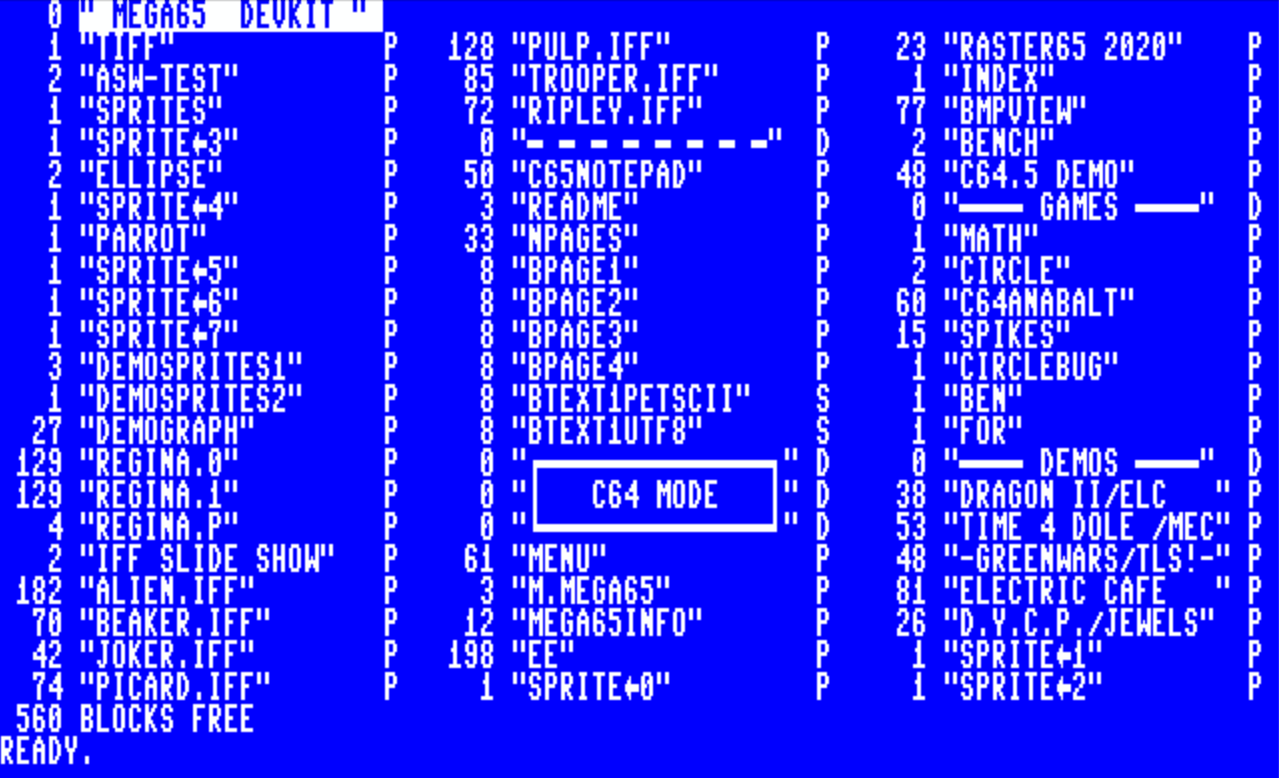
\includegraphics[width=\linewidth]{images/directory.png}
\end{description}

% ******
% CHANGE
% ******

\newpage
\subsection{CHANGE}
\index{CHANGE}
\index{BASIC 65 Commands!CHANGE}
\begin{description}[leftmargin=2cm,style=nextline]
\item [Token:] \$FE \$2C
\item [Format:] {\bf CHANGE "find" TO "replace" [,from-to]}
\item [Usage:]  Used
                in direct mode only. It searches the line range
                if specified or the whole BASIC program else.
                At each occurrence of the "find string" the line is
                listed and the user prompted for an action: \\
                'Y' <RETURN> do the change and find next string \\
                'N' <RETURN> do {\bf not} change and find next string \\
                '*' <RETURN> change this and all following matches \\
                    <RETURN> exit command, don't change.
                \item [Remarks:] Instead of the quote (\screentext{"})
                  each other character may be used
                 as delimiter for the findstring and replacestring.
                 Using the quote as delimiter finds text strings, that are
                 not tokenised and therefore not part of a keyword. \\
                 \screentext{CHANGE "LOOP" TO "OOPS"} will not find
                 the BASIC keyword \screentext{LOOP}, because the
                 keyword is stored as token and not as text.
                 However \screentext{CHANGE \&LOOP\& TO \&OOPS\&} will
                 find and replace it (probably spoiling the program).


\item [Example:] Using {\bf CHANGE}
\begin{tcolorbox}[colback=black,coltext=white]
\verbatimfont{\codefont}
\begin{verbatim}
CHANGE "XX$" TO "UU$", 2000-2700
CHANGE &IN& TO &OUT&
\end{verbatim}
\end{tcolorbox}
\end{description}

% ****
% CHAR
% ****

\newpage
\subsection{CHAR}
\index{CHAR}
\index{BASIC 65 Commands!CHAR}
\begin{description}[leftmargin=2cm,style=nextline]
\item [Token:] \$E0
\item [Format:] {\bf CHAR column, row, height, width, direction, string
                [, address of character set]}
\item [Usage:]  Displays text on a graphic screen.
                It can be used for all resolutions.

                {\bf column} is the start position of the output
                in horizontal direction.
                One column is 8 pixels wide, so a screen width of 320
                has a column range 0 -> 39, while a width of 640
                has a range of 0 -> 79.

                {\bf row} is the start position of the output
                in vertical direction. Other than column, its unit is
                pixel with top row having the value 0.

                {\bf height} is a factor applied to the vertical
                size of the characters. 1 is normal size (8 pixels)
                2 is double size (16 pixels), and so on.

                {\bf width} is a factor applied to the horizontal
                size of the characters. 1 is normal size (8 pixels)
                2 is double size (16 pixels), and so on.

                {\bf direction} controls the printing direction: \\
                1: up     \\
                2: right  \\
                4: down   \\
                8: left

                The optional {\bf address of character set} can be used
                to select a character set different from the default
                character set at \$29800, which is the set with
                upper/lower characters.

                {\bf string} is a string constant or expression
                which will be printed. This string may optionally contain
                one or more of the following control characters:

                {\setlength{\tabcolsep}{1mm}

                \ttfamily
                \begin{tabular}{|l|l|l|}
                  \hline
                     CHR\$(6)       &  CTRL+F         &  flip character \\
                     CHR\$(18)      &  RVSON          &  reverse  \\
                     CHR\$(146)     &  RVSOFF         &  reverse off \\
                     CHR\$(21)      &  CTRL+U         &  underline\\
                     CHR\$(25)+"-"  &  CTRL+Y + "-"   &  rotate left\\
                     CHR\$(25)+"+"  &  CTRL+Y + "+"   &  rotate right\\
                     CHR\$(26)      &  CTRL+Z         &  mirror\\
                  \hline
                  \end{tabular}
                }

\item [Remarks:]
                Regular text mode control characters,
                for example: cursor movement codes, will be ignored
                (neither printed nor interpreted).


\item [Example:] Using {\bf CHAR}
\begin{tcolorbox}[colback=black,coltext=white]
\verbatimfont{\codefont}
\begin{verbatim}
CHAR 304,196, 1,1,2,  "MEGA65"
\end{verbatim}
\end{tcolorbox}
will print the text "MEGA65" on the centre of a 640 x 400 graphic screen.
\end{description}

% ****
% CHR$
% ****

\newpage
\subsection{CHR\$}
\index{CHR\$}
\index{BASIC 65 Functions!CHR\$}
\begin{description}[leftmargin=2cm,style=nextline]
\item [Token:] \$C1
\item [Format:] {\bf CHR\$(numeric expression)}
\item [Usage:] Returns a string of length one character
               using the argument to insert the character having this
               value as PETSCII code.

\item [Remarks:] The argument range is 0 -> 255, so this function may
                 also be used to insert control codes into strings.
                 Even the NULL character, with code 0, is allowed. \\
               {\bf CHR\$} is the inverse function to {\bf ASC}.
\item [Example:] Using {\bf CHR\$}
\begin{tcolorbox}[colback=black,coltext=white]
\verbatimfont{\codefont}
\begin{verbatim}
10 QUOTE$   = CHR$(34)
20 ESCAPE$  = CHR$(27)
30 PRINT QUOTE$;"MEGA65";QUOTE$ : REM PRINT "MEGA65"
40 PRINT ESCAPE$;"Q";       : REM CLEAR TO END OF LINE
\end{verbatim}
\end{tcolorbox}
\end{description}

% ******
% CIRCLE
% ******

\newpage
\subsection{CIRCLE}
\index{CIRCLE}
\index{BASIC 65 Commands!CIRCLE}
\begin{description}[leftmargin=2cm,style=nextline]
\item [Token:] \$E2
\item [Format:] {\bf CIRCLE xcentre, ycentre, radius, [,solid]}
\item [Usage:] A special case of
               the {\bf ELLIPSE} command using the same value for
               horizontal and vertical radius.

               {\bf xcentre} x coordinate of centre in pixels.

               {\bf ycentre} y coordinate of centre in pixels.

               {\bf radius} radius of the circle in pixels.

               {\bf solid} will fill the circle if not zero.

\item [Remarks:] The {\bf CIRCLE} command is used to draw circles on
               screens with an aspect ratio 1:1 (for example: 320 x 200
               or 640 x 400). On other resolutions (like: 640 x 200)
               the shape will degrade to an ellipse.

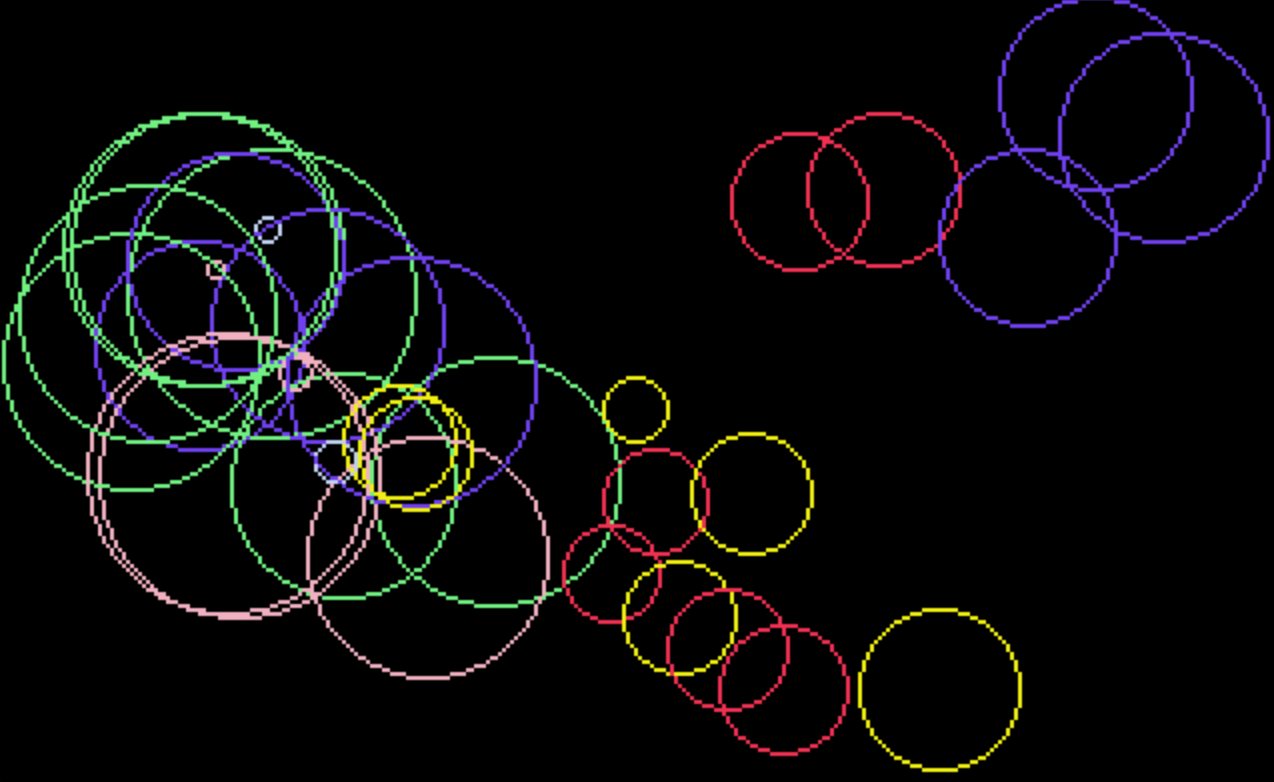
\includegraphics[width=\linewidth]{images/circle.png}
\newpage

\item [Example:] Using {\bf CIRCLE}
\begin{tcolorbox}[colback=black,coltext=white]
\verbatimfont{\codefont}
\begin{verbatim}
100 REM CIRCLE (AFTER F.BOWEN)
110 H=0:W=0                             :REM 320 X 200
120 BORDER 0                            :REM BLACK
130 GRAPHIC CLR                         :REM INIT
140 SCREEN DEF  1,W,H,4                 :REM SCREEN SETUP
150 SCREEN OPEN 1                       :REM OEN
160 PALETTE 1,0,0,0,0                   :REM BLACK
170 PALETTE 1,1,RND(.)*16,RND(.)*16,15  :REM RANDOM COLOURS
180 PALETTE 1,2,RND(.)*16,15,RND(.)*16
190 PALETTE 1,3,15,RND(.)*16,RND(.)*16
200 PALETTE 1,4,RND(.)*16,RND(.)*16,15
210 PALETTE 1,5,RND(.)*16,15,RND(.)*16
220 PALETTE 1,6,15,RND(.)*16,RND(.)*16
230 SCREEN SET 1,1                      :REM DRAW & VIEW
240 SCNCLR 0                            :REM CLEAR
250 FORI=0TO32                          :REM CIRCLE LOOP
260 PEN 0,RND(.)*6+1                    :REM RANDOM PEN
270 R=RND(.)*36+1                       :REM RADIUS
280 XC=R+RND(.)*320:IF(XC+R)>319THEN280 :REM X CENTRE
290 YC=R+RND(.)*200:IF(YC+R)>199THEN290 :REM Y CENTRE
300 XC=XC+WT*320:YC=YC+HT*200
310 CIRCLE XC,YC,R,.                    :REM DRAW
320 NEXT
330 GETKEY A$                           :REM WAIT FOR KEY
340 SCREENCLOSE 1:BORDER 6: PALETTE RESTORE
\end{verbatim}
\end{tcolorbox}
\end{description}

% *****
% CLOSE
% *****

\newpage
\subsection{CLOSE}
\index{CLOSE}
\index{BASIC 65 Commands!CLOSE}
\begin{description}[leftmargin=2cm,style=nextline]
\item [Token:] \$A0
\item [Format:] {\bf CLOSE channel}
\item [Usage:] Closes an input or output
               channel, that was established before by an {\bf OPEN}
               command.

               {\bf channel} is a value in the range 0 -> 255.

\item [Remarks:] Closing open files before the program stops is
               very important, especially for output files.
               This command flushes output buffers and
               updates directory information on disks.
               Failing to {\bf CLOSE}  can corrupt files and disks.
               BASIC does NOT automatically close channels or files
               when the program stops.

\item [Example:] Using {\bf CLOSE}
\begin{tcolorbox}[colback=black,coltext=white]
\verbatimfont{\codefont}
\begin{verbatim}
10 OPEN 2,8,2,"TEST,S,W"
20 PRINT#2,"TESTSTRING"
30 CLOSE 2 : REM OMITTING CLOSE GENERATES A SPLAT FILE
\end{verbatim}
\end{tcolorbox}
\end{description}

% ***
% CLR
% ***

\newpage
\subsection{CLR}
\index{CLR}
\index{BASIC 65 Commands!CLR}
\begin{description}[leftmargin=2cm,style=nextline]
\item [Token:] \$9C
\item [Format:] {\bf CLR}        \\
                {\bf CLR DS\$}   \\
                {\bf CLR ERR\$}
\item [Usage:] {\bf CLR} with no parameters Resets all pointers, that
               are used for management of BASIC variables, arrays
               and strings. The run-time stack pointers are reset
               and the table of open channels is reset.
               A {\bf RUN} command performs {\bf CLR} automatically.

               {\bf CLR DS\$} clears the currently buffered disk status.
               Any reference to {\bf DS} or {\bf DS\$} after clearing
               will read the status from the disk device.

               {\bf CLR ERR\$} clears the program error status.
               This command is typically used in a {\bf TRAP} handler,
               which has resolved an error and calls {\bf RESUME}.

\item [Remarks:] {\bf CLR} should not be used inside loops or
               subroutines because it destroys the return address.
               After a {\bf CLR} all variables are unknown and will
               be initialised at the next usage.

\item [Example:] Using {\bf CLR}
\begin{tcolorbox}[colback=black,coltext=white]
\verbatimfont{\codefont}
\begin{verbatim}
10 A=5: P$="MEGA65"
20 CLR
30 PRINT A;P$

0
READY.
CLR DS$
PRINT DS$
00,OK,00,00
\end{verbatim}
\end{tcolorbox}
\end{description}

% ***
% CMD
% ***

\newpage
\subsection{CMD}
\index{CMD}
\index{BASIC 65 Commands!CMD}
\begin{description}[leftmargin=2cm,style=nextline]
\item [Token:] \$9D
\item [Format:] {\bf CMD channel [,string]}
\item [Usage:] Redirects the standard output
               from screen to the channel. This enables to
               print listings and directories or other screen outputs.
               It is also possible to redirect this output to a disk file
               or a modem.

               {\bf channel} must be opened by the {\bf OPEN} command.

               The optional {\bf string} is sent to the channel
               before the redirection begins and can be used,
               for example, for printer setup escape sequences.

\item [Remarks:] The {\bf CMD} mode is stopped by a {\bf PRINT\# channel}
                 or by closing the channel with {\bf CLOSE channel}.
                 It is recommended to use a {\bf PRINT\# channel}
                 before closing, to make sure, that the output buffer
                 is flushed.

\item [Example:] Using {\bf CMD} to print a program listing:
\begin{tcolorbox}[colback=black,coltext=white]
\verbatimfont{\codefont}
\begin{verbatim}
OPEN 1,4    :REM OPEN CHANNEL #1 TO PRINTER AT UNIT 4
CMD 1
LIST
PRINT#1
CLOSE 1
\end{verbatim}
\end{tcolorbox}
\end{description}

% *******
% COLLECT
% *******

\newpage
\subsection{COLLECT}
\index{COLLECT}
\index{BASIC 65 Commands!COLLECT}
\begin{description}[leftmargin=2cm,style=nextline]
\item [Token:] \$F3
\item [Format:] {\bf COLLECT [,D drive] [,U unit] }
\item [Usage:]
   Rebuilds the {\bf BAM}
   (Block Availability Map) deleting splat files and marking
   unused blocks as free.

   \drivedefinition

   \unitdefinition

\item [Remarks:]
   While this command is useful for cleaning the disk from
   splat files (for example: write files, that weren't properly closed)
   it is dangerous for disks with boot blocks or random access files.
   These blocks are not associated with standard disk files
   and will therefore be marked as free too and may be overwritten
   by further disk write operations.

\item [Example:] Using {\bf COLLECT}
\begin{tcolorbox}[colback=black,coltext=white]
\verbatimfont{\codefont}
\begin{verbatim}
  COLLECT
  COLLECT U9
  COLLECT D0, U9
\end{verbatim}
\end{tcolorbox}
\end{description}

% *********
% COLLISION
% *********

\newpage
\subsection{COLLISION}
\index{COLLISION}
\index{BASIC 65 Commands!COLLISION}
\begin{description}[leftmargin=2cm,style=nextline]
\item [Token:] \$FE \$17
\item [Format:] {\bf COLLISION type [,linenumber]}
\item [Usage:]  Enables or disables
                an user programmed interrupt handler.
                A call without linenumber disables the handler,
                while a call with linenumber enables it.
                After the execution of {\bf COLLISION} with
                linenumber a sprite collision of the same type,
                as specified in the {\bf COLLISION} call,
                interrupts the BASIC program and perform a {\bf GOSUB}
                to {\bf linenumber} which is expected to contain
                the user code for handling sprite collisions.
                This handler must give control back with a {\bf RETURN}.

                {\bf type} specifies the collision type for
                this interrupt handler: \\
                1 = sprite - sprite collision \\
                2 = sprite - data - collision \\
                3 = light pen

                {\bf linenumber} must point to a subroutine
                which holds code for handling sprite collision
                and ends with a {\bf RETURN}.

\item [Remarks:] It is possible to enable interrupt handler for
               all types, but only one can execute at any time.
               A interrupt handler cannot be interrupted by another
               interrupt handler.
               Functions like {\bf BUMP}, {\bf RSPPOS} and
               {\bf LPEN} may be used for evaluation of the sprites
               which are involved and their positions.

\item [Example:] Using {\bf COLLISION}
\begin{tcolorbox}[colback=black,coltext=white]
\verbatimfont{\codefont}
\begin{verbatim}
10 COLLISION 1,70 : REM ENABLE
20 SPRITE 1,1 : MOVSPR 1,120,  0 : MOVSPR 1,0#5
30 SPRITE 2,1 : MOVSPR 2,120,100 : MOVSPR 2,180#5
40 FOR I=1 TO 50000:NEXT
50 COLLISION 1 : REM DISABLE
50 END
70 REM SPRITE <-> SPRITE INTERRUPT HANDLER
80 PRINT "BUMP RETURNS";BUMP(1)
90 RETURN: REM RETURN FROM INTERRUPT
\end{verbatim}
\end{tcolorbox}
\end{description}

% *****
% COLOR
% *****

\newpage
\subsection{COLOR}
\index{COLOR}
\index{BASIC 65 Commands!COLOR}
\begin{description}[leftmargin=2cm,style=nextline]
\item [Token:] \$E7
\item [Format:] {\bf COLOR <ON|OFF>}
\item [Usage:] Enables or disables
               handling of the character attributes on the screen.
               If {\bf COLOR} is {\bf ON}, the screen routines
               take care for both character RAM and attribute RAM.
               E.g. if the screen is scrolled for text, the attributes
               are scrolled too, so each character keeps his attribute
               or colour. If {\bf COLOR} is {\bf OFF}, the attribute
               or colour RAM is fixed and character movement is only
               done for screen characters. This speeds up screen
               handling, if moving characters with different colours is
               not intended.
\item [Example:] \screentext{COLOR ON} - with colour/attribute handling \\
                 \screentext{COLOR OFF} - no colour/attribute handling

\end{description}

% ******
% CONCAT
% ******

\newpage
\subsection{CONCAT}
\index{CONCAT}
\index{BASIC 65 Commands!CONCAT}
\begin{description}[leftmargin=2cm,style=nextline]
\item [Token:] \$FE \$13
\item [Format:] {\bf CONCAT appendfile [,D drive] TO
                targetfile [,D drive] [,U unit] }
\item [Usage:]
   The {\bf CONCAT} (concatenation) appends the contents of
   {\bf appendfile} to the {\bf targetfile}. Afterwards {\bf targetfile}
   contains the contents of both files, while {\bf appendfile}
   remains unchanged.

   {\bf appendfile} is either a quoted string, for example: {\bf "data"} or
   a string expression in parentheses, for example: {\bf (FI\$)}

   {\bf targetfile} is either a quoted string, for example: {\bf "safe"} or
   a string expression in parentheses, for example: {\bf (FS\$)}

   If the disk unit has dual drives, it is possible to apply
   the {\bf CONCAT} command to files, which are stored on different
   disks. In this case, it is necessary to specify the drive\#
   for both files in the command. This is necessary too, if both
   files are stored on drive\#1.

   \drivedefinition

   \unitdefinition

\item [Remarks:]
   The {\bf CONCAT} commands is executed in the DOS of the disk drive.
   Both files must exist and no pattern matching is allowed.
   Only sequential files of type {\bf SEQ} may be concatenated.

\item [Example:] Using {\bf CONCAT}
\begin{tcolorbox}[colback=black,coltext=white]
\verbatimfont{\codefont}
\begin{verbatim}
  CONCAT "NEW DATA" TO "ARCHIVE" ,U9
  CONCAT "ADDRESS",D0 TO "ADDRESS BOOK",D1
\end{verbatim}
\end{tcolorbox}
\end{description}

% ****
% CONT
% ****

\newpage
\subsection{CONT}
\index{CONT}
\index{BASIC 65 Commands!CONT}
\begin{description}[leftmargin=2cm,style=nextline]
\item [Token:] \$9A
\item [Format:] {\bf CONT}
\item [Usage:] Used to resume
               program execution after a break or stop caused by
               an {\bf END} or {\bf STOP} statement or by pressing
               the {\bf STOP KEY}.
               This is a useful debug tool. The BASIC program may be stopped
               and variables can be examined and even changed.
               The {\bf CONT} statement then resumes execution.
\item [Remarks:] {\bf CONT} cannot be used, if the program stops
               due to errors. Also any editing of the program
               inhibits continuation. Stopping and continuation
               can spoil the screen output or interfere with
               input/output operations.
\item [Example:] Using {\bf CONT}
\begin{tcolorbox}[colback=black,coltext=white]
\verbatimfont{\codefont}
\begin{verbatim}
10 I=I+1:GOTO 10
RUN

BREAK IN 10
READY.
PRINT I
 947
CONT
\end{verbatim}
\end{tcolorbox}
\end{description}

% ****
% COPY
% ****

\newpage
\subsection{COPY}
\index{COPY}
\index{BASIC 65 Commands!COPY}
\begin{description}[leftmargin=2cm,style=nextline]
\item [Token:] \$F4
\item [Format:] {\bf COPY source [,D drive] [,U unit] TO
                target [,D drive] [,U unit] }
\item [Usage:]
   Copies the contents of
   {\bf source} to the {\bf target}.
   It is used to copy either single files or, by using
   wildcard characters, multiple files.

   {\bf source} is either a quoted string, e.g. {\bf "data"} or
   a string expression in parentheses, e.g. {\bf (FI\$)}.

   {\bf target} is either a quoted string, e.g. {\bf "backup"} or
   a string expression in parentheses, e.g. {\bf (FS\$)}

   \drivedefinition

   \unitdefinition

   If none or one unit number is given or the unit numbers before and after
   the TO token are equal, the COPY command is executed inside the disk unit
   and the source and target files are on the same disk.

   If the source unit (before TO) is different to the target unit (after TO),
   the COPY command is executed in the MEGA65 BASIC by reading the source
   files into a RAM buffer and writing to the target unit. In this case
   the target file name cannot be chosen, but will be the same as the
   destination filename. The extended unit to unit copy mode allows to copy
   single files, pattern matching files or all files of a disk.
   Any combination of units is allowed, internal floppy, SD-card images,
   IEC floppy drives like 1541, 1571, 1581 or CMD floppy and hard drives.

\item [Remarks:]
   The file types PRG, SEQ and USR can be copied.
   If source and target are on the same disk, the target filename
   must be different from the source file name.

   The COPY command cannot copy {\bf DEL} files, that are commonly used
   as title or separators in disk directories. These do not conform to
   Commodore DOS rules and cannot be accessed by standard OPEN routines.

   {\bf REL} files cannot be copied from unit to unit.

\item [Example:] Using {\bf COPY}
\begin{tcolorbox}[colback=black,coltext=white]
\verbatimfont{\codefont}
\begin{verbatim}
  COPY U8 TO U9            :REM COPY ALL FILES
  COPY "CODES" TO "BACKUP" :REM COPY SINGLE FILE
  COPY "*.TXT",U8 TO U9    :REM PATTERN COPY
  COPY "M*",U9 TO U11      :REM PATTERN COPY
\end{verbatim}
\end{tcolorbox}
\end{description}

% ***
% COS
% ***

\newpage
\subsection{COS}
\index{COS}
\index{BASIC 65 Functions!COS}
\begin{description}[leftmargin=2cm,style=nextline]
\item [Token:] \$BE
\item [Format:] {\bf COS(numeric expression)}
\item [Usage:] The {\bf COS} function returns the cosine of the
               argument.
               The argument is expected in units of {\bf [radians]}.
               The result is in the range (-1.0 to +1.0)

\item [Remarks:] An argument in units of {\bf [degrees]}
                 can be converted to {\bf [radians]}
               by multiplication with $\pi/180$.
\item [Example:] Using {\bf COS}
\begin{tcolorbox}[colback=black,coltext=white]
\verbatimfont{\codefont}
\begin{verbatim}
  PRINT COS(0.7)
   .764842187

  X=60:PRINT COS(X * ~ / 180)
   .500000001
\end{verbatim}
\end{tcolorbox}
\end{description}

% ******
% CURSOR
% ******

\newpage
\subsection{CURSOR}
\index{CURSOR}
\index{BASIC 65 Commands!CURSOR}
\begin{description}[leftmargin=2cm,style=nextline]
%\item [Token:] \$??
\item [Format:] {\bf CURSOR [<ON/OFF>] [,column] [,row] [,style]}
\item [Usage:] Moves the text cursor to
               the specified position on the current text screen.

               {\bf ON} or {\bf OFF} displays or hides the cursor.

               {\bf column} and {\bf row} specify the new position.

               {\bf style} defines a solid (1) or flashing (0) cursor.

%\item [Remarks:]
\item [Example:] Using {\bf CURSOR}
\begin{tcolorbox}[colback=black,coltext=white]
\verbatimfont{\codefont}
\begin{verbatim}
10 CURSOR ON,1,2,1 :REM SET SOLID CURSOR AT COLUMN 1, ROW 2
\end{verbatim}
\end{tcolorbox}
\end{description}

% ****
% DATA
% ****

\newpage
\subsection{DATA}
\index{DATA}
\index{BASIC 65 Commands!DATA}
\begin{description}[leftmargin=2cm,style=nextline]
\item [Token:] \$83
\item [Format:] {\bf DATA [list of constants]}
\item [Usage:] Used to define constants
               which can be read by {\bf READ} statements somewhere
               in the program. Numbers and strings are allowed, but no expressions.
               Items are separated by commas.
               Strings containing commas, colons or spaces must be put
               in quotes. \\
               A {\bf RUN} command initialises the data pointer
               to the first item of the first {\bf DATA} statement
               and advances it for every read item. It is in the
               responsibility of the programmer, that the type of
               the constant and the variable in the {\bf READ}
               statement match. Empty items with no constant
               between commas are allowed and will be interpreted as
               zero for numeric variables and an empty string for
               string variables. \\
               The {\bf RESTORE} command may be used to set the
               data pointer to a specific line for subsequent
               readings.

\item [Remarks:] It is good programming style to put large amount of
               {\bf DATA} statements at the end of the program.
               Otherwise they slow down the search for line numbers
               after {\bf GOTO} and other statements with targets.
\item [Example:] Using {\bf DATA}
\begin{tcolorbox}[colback=black,coltext=white]
\verbatimfont{\codefont}
\begin{verbatim}
1 REM DATA
10 READ NA$, VE
20 READ N% : FOR I=2 TO N% : READ GL(I) : NEXT I
30 PRINT "PROGRAM:";NA$;"  VERSION:";VE
40 PRINT "N-POINT GAUSSLEGENDRE FACTORS E1":
50 FOR I=2 TO N%:PRINT I;GL(I):NEXT I
60 END
80 DATA "MEGA65",1.1
90 DATA 5,0.5120,0.3573,0.2760,0.2252

RUN
PROGRAM:MEGA65  VERSION: 1.1
N-POINT GAUSSLEGENDRE FACTORS E1
 2  0.512
 3  0.3573
 4  0.276
 5  0.2252
\end{verbatim}
\end{tcolorbox}
\end{description}

% ******
% DCLEAR
% ******

\newpage
\subsection{DCLEAR}
\index{DCLEAR}
\index{BASIC 65 Commands!DCLEAR}
\begin{description}[leftmargin=2cm,style=nextline]
\item [Token:] \$FE \$15
\item [Format:] {\bf DCLEAR [,D drive] [,U unit] }
\item [Usage:]
   Sends an initialise command to
   the specified unit and drive.

   \drivedefinition

   \unitdefinition

\item [Remarks:]
   The DOS inside the disk unit will close all open files,
   clear all channels, free buffers and reread the BAM.
   This command should be used together with a {\bf DCLOSE}
   to make sure, that the computer and the drive agree
   on the status, otherwise strange side effects may occur.

\item [Example:] Using {\bf DCLEAR}
\begin{tcolorbox}[colback=black,coltext=white]
\verbatimfont{\codefont}
\begin{verbatim}
  DCLOSE   :DCLEAR
  DCLOSE U9:DCLEAR U9
  DCLOSE U9:DCLEAR D0, U9
\end{verbatim}
\end{tcolorbox}
\end{description}

% ******
% DCLOSE
% ******

\newpage
\subsection{DCLOSE}
\index{DCLOSE}
\index{BASIC 65 Commands!DCLOSE}
\begin{description}[leftmargin=2cm,style=nextline]
\item [Token:] \$FE \$0F
\item [Format:] {\bf DCLOSE [\#channel] [,U unit] }
\item [Usage:]
   Closes a single file or
   all files for the specified unit.

   {\bf channel} = channel \# assigned with the {\bf DOPEN} statement.

   \unitdefinition

   The {\bf DCLOSE} command is used either with a channel argument
   or a unit number, but never both.

\item [Remarks:]
   It is important to close all open files before the program ends.
   Otherwise buffers will not be freed and even worse, open write
   files will be incomplete (splat files) and no more usable.

\item [Example:] Using {\bf DCLOSE}
\begin{tcolorbox}[colback=black,coltext=white]
\verbatimfont{\codefont}
\begin{verbatim}
  DCLOSE#2 :REM CLOSE FILE ASSIGNED TO CHANNEL 2
  DCLOSE U9:REM CLOSE ALL FILES OPEN ON UNIT 9
\end{verbatim}
\end{tcolorbox}
\end{description}

% ***
% DEC
% ***

\newpage
\subsection{DEC}
\index{DEC}
\index{BASIC 65 Functions!DEC}
\begin{description}[leftmargin=2cm,style=nextline]
\item [Token:] \$D1
\item [Format:] {\bf DEC(string expression)}
\item [Usage:] Returns the decimal value
               of the argument, that is written as a hex string.
               The argument range is "0000" to "FFFF" or
               0 to 65535 respectively.
               The argument must have 1-4 hex digits.

\item [Remarks:] Allowed digits in uppercase/graphics mode are: \\
                 0123456789ABCDEF and in lowercase/uppercase mode: \\
                 0123456789abcdef.

\item [Example:] Using {\bf DEC}
\begin{tcolorbox}[colback=black,coltext=white]
\verbatimfont{\codefont}
\begin{verbatim}
  PRINT DEC("D000")
   53248
  POKE DEC("600"),255
\end{verbatim}
\end{tcolorbox}
\end{description}

% ***
% DEF
% ***

\newpage
\subsection{DEF FN}
\index{DEF FN}
\index{BASIC 65 Commands!DEF FN}
\index{FN}
\index{BASIC 65 Functions!FN}
\begin{description}[leftmargin=2cm,style=nextline]
\item [Token:] \$96
\item [Format:] {\bf DEF FN name(real variable)}
\item [Usage:] Defines a single statement
               user function with one argument of real type
               returning a real value.
               The definition must be executed before the function
               can be used in expressions. The argument is
               a dummy variable, which will be replaced by the
               argument in the function usage.

\item [Remarks:] The value of the dummy variable will not be changed
                 and the variable may be used in other context
                 without side effects.

\item [Example:] Using {\bf DEF FN}
\begin{tcolorbox}[colback=black,coltext=white]
\verbatimfont{\codefont}
\begin{verbatim}
10 PD = ~ / 180
20 DEF FN CD(X)= COS(X*PD): REM COS FOR DEGREES
30 DEF FN SD(X)= SIN(X*PD): REM SIN FOR DEGREES
40 FOR D=0 TO 360 STEP 90
50 PRINT USING "###";D
60 PRINT USING " ##.##";FNCD(D);
70 PRINT USING " ##.##";FNSD(D)
80 NEXT D
RUN
  0  1.00  0.00
 90  0.00  1.00
180 -1.00  0.00
270  0.00 -1.00
360  1.00  0.00
\end{verbatim}
\end{tcolorbox}
\end{description}

% ******
% DELETE
% ******

\newpage
\subsection{DELETE}
\index{DELETE}
\index{BASIC 65 Commands!DELETE}
\begin{description}[leftmargin=2cm,style=nextline]
\item [Token:] \$F7
\item [Format:] {\bf DELETE [line range]} \\
                {\bf DELETE filename [,D drive] [,U unit] [,R]}
\item [Usage:] Used either to delete
               a range of lines from the BASIC program or
               to delete a disk file.

               {\bf line range} consist of the first and the last
               line to delete or a single line number.
               If the first number is omitted, the
               first BASIC line is assumed.
               The second number in the range specifier defaults
               to the last BASIC line.

   {\bf filename} is either a quoted string, for example: {\bf "safe"} or
   a string expression in parentheses, for example: {\bf (FS\$)}

   \drivedefinition

   \unitdefinition

   {\bf R} = Recover a previously deleted file.
   This will only work, if there were no write operations
   between deletion and recovery, which may have altered the
   contents of the file.

\item [Remarks:] The {\bf DELETE filename} command works like the
                 {\bf SCRATCH filename} command.

\item [Example:] Using {\bf DELETE}
\begin{tcolorbox}[colback=black,coltext=white]
\verbatimfont{\codefont}
\begin{verbatim}
  DELETE 100      :REM DELETE LINE 100
  DELETE 240-350  :REM DELETE ALL LINES FROM 240 TO 350
  DELETE 500-     :REM DELETE FROM 500 TO END
  DELETE -70      :REM DELETE FROM START TO 70

  DELETE "DRM",U9 :REM DELETE FILE DRM ON UNIT 9
\end{verbatim}
\end{tcolorbox}
\end{description}

% ***
% DIM
% ***

\newpage
\subsection{DIM}
\index{DIM}
\index{BASIC 65 Commands!DIM}
\begin{description}[leftmargin=2cm,style=nextline]
\item [Token:] \$86
\item [Format:] {\bf DIM name(limits) [,name(limits)]...}
\item [Usage:] Declares the shape,
               the bounds and the type of a BASIC array.
               As a declaration statement it must be executed
               only once and before any usage of the declared arrays.
               An array can have one or more dimensions.
               One dimensional arrays are often called vectors
               while two or more dimensions define a matrix.
               The lower bound of a dimension is always zero,
               while the upper bound is declared. The rules for
               variable names apply for array names too.
               There are integer arrays, real arrays and string arrays.
               It is legal to use the same identifier for scalar
               variables and array variables. The left parenthesis
               after the name identifies array names.

\item [Remarks:] Integer arrays consume two bytes per element,
                 real arrays five bytes and string arrays three bytes
                 for the string descriptor plus
                 the length of the string. \\
                 If an array identifier is used without previous
                 declaration, an implicit declaration of an
                 one dimensional array with limit 10 is performed.

\item [Example:] Using {\bf DIM}
\begin{tcolorbox}[colback=black,coltext=white]
\verbatimfont{\codefont}
\begin{verbatim}
10 DIM A%(8)   :REM ARRAY OF 9 ELEMENTS
20 DIM XX(2,3) :REM ARRAY OF 3x4 = 12 ELEMENTS
30 FOR I=0 TO 8:A%(I)=PEEK(256+I):NEXT
40 FOR I=0 TO 2:FOR J=0 TO 3:READ XX(I,J):NEXT J,I
50 END
60 DATA 1,-2,3,-4,5,-6,7,-8,9,-10,11,-12
\end{verbatim}
\end{tcolorbox}
\end{description}

% ***
% DIR
% ***

\newpage
\subsection{DIR}
\index{DIR}
\index{BASIC 65 Commands!DIR}
\begin{description}[leftmargin=2cm,style=nextline]
\item [Token:] \$EE (DIR) \$FE \$29 (ECTORY)
\item [Format:] {\bf DIRECTORY [filepattern] [,W] [,R] [,D drive] [,U unit] }
\item [Format:] {\bf DIR [filepattern] [,W] [,R] [,D drive] [,U unit] }
\item [Format:] {\bf \$ [filepattern] [,W] [,R] [,D drive] [,U unit] }
\item [Usage:]  Prints a file directory/catalog of the specified disk.

   The shortcut symbol {\bf \$} can be used in direct mode only.

   The {\bf W} (Wide) parameter lists the directory three columns wide
   on the screen and pauses after a the screen is full (63 directory
   entries). Pressing any key displays the next page.

   The {\bf R} (Recoverable) parameter includes files in the
   directory, which are flagged as deleted but are still
   recoverable.

   {\bf filepattern} is either a quoted string, for example: {\bf "da*"} or
   a string expression in parentheses, e.g. {\bf (DI\$)}

   \drivedefinition

   \unitdefinition

\item [Remarks:]
   The command {\bf DIR} is a synonym for {\bf CATALOG}
   or {\bf DIRECTORY} and produces the same listing.
   The {\bf filepattern} can be used to filter the listing.
   The wildcard characters {\bf *} and {\bf ?} may be used.
   Adding a {\bf ,T=} to the pattern string, with {\bf T} specifying
   a filetype of {\bf P}, {\bf S}, {\bf U} or {\bf R}
   (for {\bf P}RG, {\bf S}EQ, {\bf U}SR, {\bf R}EL) filters the
   output to that filetype.

\item [Example:] Using {\bf DIRECTORY}

% Character test

%\begin{tcolorbox}[colback=black,coltext=white]
%\verbatimfont{\codefont}
%\begin{verbatim}
%
% !"#$%&'()*+,-./
%0123456789:;<=>?
%@ABCDEFGHIJKLMNO
%PQRSTUVWXYZ[\]^_
%`abcdefghijklmno
%pqrstuvwxyz{|}~
%
%ÀÁÂÃÄÅÆÇÈÉÊËÌÍÎÏ
%ÐÑÒÓÔÕÖ×ØÙÚÛÜÝÞß
%àáâãäåæçèéêëìíîï
%ðñòóôõö÷øùúûüýþÿ
%
%ĀāĂ㥹ĆćĈĉĊċČčĎď
%ĐđĒēĔĕĖėĘęĚěĜĝĞğ
%ĠġĢģĤĥĦħĨĩĪīĬĭĮį
%İıIJijĴĵĶķĸĹĺĻļĽľĿ
%
%ŀŁłŃńŅņŇňʼnŊŋŌōŎŏ
%ŐőŒœŔŕŖŗŘřŚśŜŝŞş
%ŠšŢţŤťŦŧŨũŪūŬŭŮů
%ŰűŲųŴŵŶŷŸŹźŻżŽžſ
%
%\end{verbatim}
%\end{tcolorbox}

\begin{tcolorbox}[colback=black,coltext=white]
\verbatimfont{\codefont}
\begin{verbatim}
DIRECTORY
\end{verbatim}
\selectfont{\codefont 0}
\begin{tcolorbox}[colback=white,coltext=black,arc=0mm,boxrule=0mm,
       left*=0.5mm,right*=0mm,top=0mm,bottom=0mm,nobeforeafter,
       left skip=0.5mm,
       width=28mm,height=3mm,valign=center]
\begin{verbatim}
"BLACK SMURF     " BS 2A
\end{verbatim}
\end{tcolorbox}
\begin{verbatim}
508  "STORY PHOBOS"     SEQ
27   "C8096"            PRG
25   "C128"             PRG
104 BLOCKS FREE.
\end{verbatim}
\end{tcolorbox}

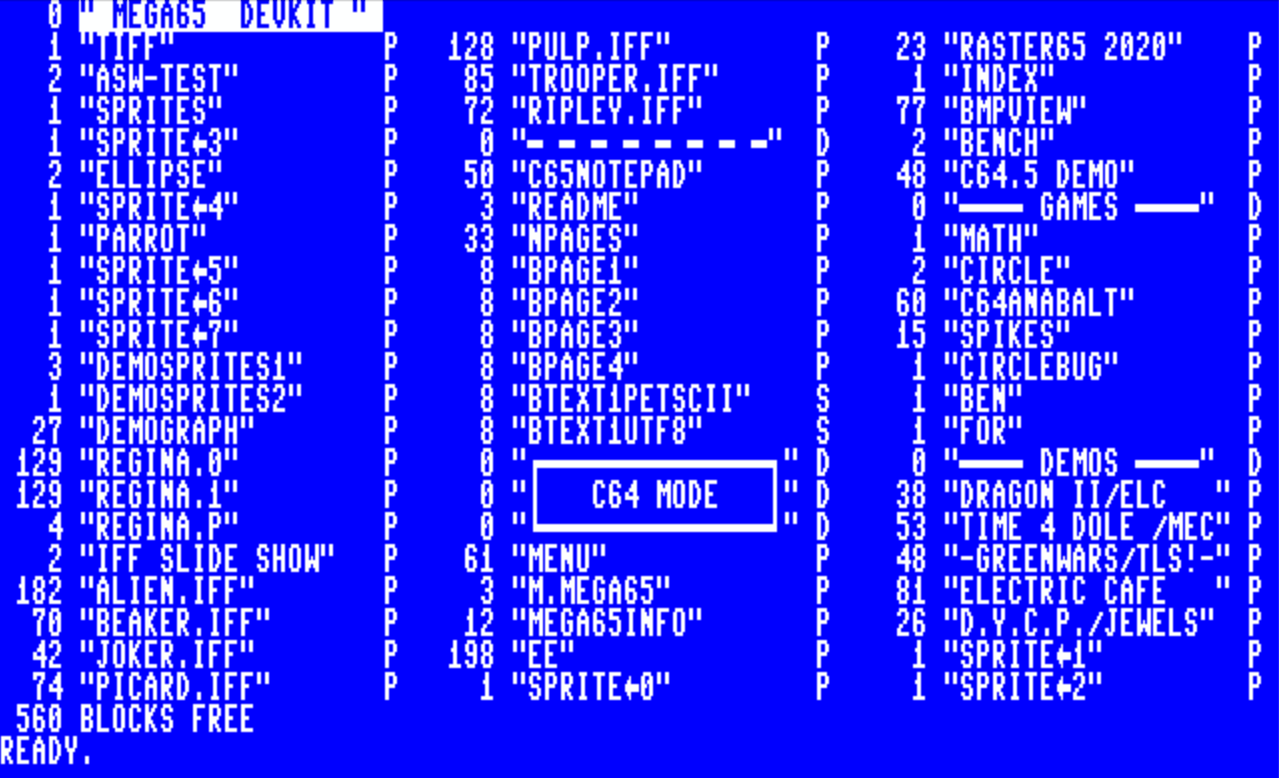
\includegraphics[width=\linewidth]{images/directory.png}

\end{description}

% ****
% DISK
% ****

\newpage
\subsection{DISK}
\index{DISK}
\index{BASIC 65 Commands!DISK}
\begin{description}[leftmargin=2cm,style=nextline]
\item [Token:] \$FE \$40
\item [Format:] {\bf DISK command [,U unit] }
\item [Format:] {\bf @ command [,U unit] }
\item [Usage:]

   The shortcut symbol {\bf @}  can be used in direct mode only.

   Sends a command string to the specified disk unit.

   Using the command with no parameters, prints the disk status.

   \unitdefinition

   {\bf command} is a string expression.

\item [Remarks:]
   The command string is interpreted by the disk unit
   and must be compatible to the used DOS version.
   Read the disk drive manual for possible commands.

\item [Example:] Using {\bf DISK}
\begin{tcolorbox}[colback=black,coltext=white]
\verbatimfont{\codefont}
\begin{verbatim}
  DISK "I0"   :REM INITIALISE DISK IN DRIVE 0
  DISK "U0>9" :REM CHANGE UNIT# TO 9
\end{verbatim}
\end{tcolorbox}
\end{description}

% *****
% DLOAD
% *****

\newpage
\subsection{DLOAD}
\index{DLOAD}
\index{BASIC 65 Commands!DLOAD}
\begin{description}[leftmargin=2cm,style=nextline]
\item [Token:] \$F0
\item [Format:] {\bf DLOAD filename [,D drive] [,U unit] }
\item [Usage:]
   "Disk LOAD" loads a file of type
   PRG into memory reserved for BASIC program source.

   \filenamedefinition

   \drivedefinition

   \unitdefinition

\item [Remarks:]
   The load address, stored in the first two bytes
   of the file is ignored. The program is loaded into
   the BASIC memory. This enables loading of BASIC programs,
   that were saved on other computers with different memory
   configurations. After loading the program is re-linked
   and ready to run or edit.
   It is possible to use DLOAD in a running program
   (Called overlay or chaining).
   Then the new loaded program replaces the current one
   and the execution starts automatically on the first line of the
   new program. Variables, arrays and strings from the current
   run are preserved and can be used by the new loaded program.

\item [Example:] Using {\bf DLOAD}
\begin{tcolorbox}[colback=black,coltext=white]
\verbatimfont{\codefont}
\begin{verbatim}
  DLOAD "APOCALYPSE"
  DLOAD "MEGA TOOLS",U9
  DLOAD (FI$),U(UN%)
\end{verbatim}
\end{tcolorbox}
\end{description}

% ***
% DMA
% ***

\newpage
\subsection{DMA}
\label{BASIC 65 Commands!DMA}
\index{DMA}
\index{BASIC 65 Commands!DMA}
\begin{description}[leftmargin=2cm,style=nextline]
\item [Token:] \$FE \$1F
\item [Format:] {\bf DMA command [,length, source address,
                 source bank, target address, target bank, sub]}
\item [Usage:]
   The {\bf DMA} ("Direct Memory Access") command is obolete
   and replaced by the command {\bf EDMA}.

   {\bf command} 0 = copy, 1 = mix, 2 = swap, 3 = fill

   {\bf length} = number of bytes

   {\bf source address} = 16 bit address of read area or fill byte

   {\bf source bank} = bank number for source (ignored for fill mode)

   {\bf target} = 16 bit address of write area

   {\bf target bank} = bank number for target

   {\bf sub} = sub command

\item [Remarks:]
The {\bf DMA} command has access to the lower 1 MB address range
organised in 16 banks of 64 K. To avoid this limitation, use the
command {\bf EDMA}, which has access to the full 256 MB address range.

\item [Example:] Using {\bf DMA}
\begin{tcolorbox}[colback=black,coltext=white]
\verbatimfont{\codefont}
\begin{verbatim}
DMA 0, 80*25, 2048, 0, 0, 4  :REM SAVE SCREEN TO $00000 BANK 4
DMA 3, 80*25, 32, 0, 2048, 0 :REM FILL SCREEN WITH BLANKS
DMA 0, 80*25, 0, 4, 2048, 0  :REM RESTORE SCREEN FROM $00000 BANK 4
DMA 2, 80, 2048, 0, 2048+80, 0 :REM SWAP CONTENTS OF LINE 1 & 2 OF SCREEN
\end{verbatim}
\end{tcolorbox}
\end{description}

% *****
% DMODE
% *****

\newpage
\subsection{DMODE}
\index{DMODE}
\index{BASIC 65 Commands!DMODE}
\begin{description}[leftmargin=2cm,style=nextline]
\item [Token:] \$FE \$35
\item [Format:] {\bf DMODE jam,complement,inverse,stencil,style,thick}
\item [Usage:]
   "Display MODE" sets several parameter
   of the graphical context for drawing commands.

\ttfamily
\begin{tabular}{|l|l|}
\hline
   {\bf jam}        &  0 - 1 \\
   {\bf complement} &  0 - 1 \\
   {\bf inverse}    &  0 - 1 \\
   {\bf stencil}    &  0 - 1 \\
   {\bf style}      &  0 - 3 \\
   {\bf thick}      &  1 - 8 \\
\hline
\end{tabular}
\end{description}

% **
% DO
% **

\newpage
\subsection{DO}
\index{DO}
\index{BASIC 65 Commands!DO}
\begin{description}[leftmargin=2cm,style=nextline]
\item [Token:] \$EB
\item [Format:] {\bf DO} ... {\bf LOOP} \\
                {\bf DO} [ <{\bf UNTIL | WHILE}> <logical expr.>] \\
                . . . statements [{\bf EXIT}] \\
                {\bf LOOP} [ <{\bf UNTIL | WHILE}> <logical expr.>]
\item [Usage:] The {\bf DO} and {\bf LOOP} keywords define
               the start and end of the most versatile BASIC loop.
               Using {\bf DO} and {\bf LOOP} alone, without any
               modifiers creates an infinite loop, that can be left
               by the {\bf EXIT} statement only. The loop can be
               controlled by adding an {\bf UNTIL} or a {\bf WHILE}
               statement after the {\bf DO} or {\bf LOOP}.

\item [Remarks:] {\bf DO} loops may be nested. An {\bf EXIT} statement
               exits the current loop only.
\item [Example:] Using {\bf DO} and {\bf LOOP}
\begin{tcolorbox}[colback=black,coltext=white]
\verbatimfont{\codefont}
\begin{verbatim}
10 PW$="":DO
20 GET A$:PW$=PW$+A$
30 LOOP UNTIL LEN(PW$)>7 OR A$=CHR$(13)

10 DO : REM WAIT FOR USER DECISION
20 GET A$
30 LOOP UNTIL A$='Y' OR A$='N' OR A$='y' OR A$='n'

10 DO WHILE ABS(EPS) > 0.001
20 GOSUB 2000 : REM ITERATION SUBROUTINE
30 LOOP

10 I%=0 : REM INTEGER LOOP 1 -> 100
20 DO I%=I%+1
30 LOOP WHILE I% < 101
\end{verbatim}
\end{tcolorbox}
\end{description}

% *****
% DOPEN
% *****

\newpage
\subsection{DOPEN}
\index{DOPEN}
\index{BASIC 65 Commands!DOPEN}
\begin{description}[leftmargin=2cm,style=nextline]
\item [Token:] \$FE \$0D
\item [Format:]
  {\bf DOPEN\# lfn, filename [,L[reclen]] [,W] [,D drive] [,U unit] }
\item [Usage:]
   Opens a file for reading, writing or
   modifying.

   {\bf lfn} = {\bf l}ogical {\bf f}ile {\bf n}umber \\
   1 <= lfn <= 127: line terminator is CR \\
   128 <= lfn <= 255: line terminator is CR LF

   {\bf L} indicates, that the file is a relative file, which
   is opened for read/write and random access. The reclength
   is mandatory for creating relative files. For existing
   relative files, the reclen is used as a safety check, if given.

   {\bf W} opens a file for write access. The file must not exist.

   \filenamedefinition

   \drivedefinition

   \unitdefinition

\item [Remarks:]
   \screentext{DOPEN\#} may be used to open all file types.
   The sequential file type {\bf SEQ} is default.
   The relative file type {\bf REL} is chosen by using the
   {\bf L} parameter.  Other file types
   must be specified in the filename, e.g. by adding ",P" to the
   filename for program files or ",U" for USR files.

   The usage of the "save-and-replace" character '@' at the
   beginning of the filename is not recommended, because many
   Commodore disk drives have a bug, that can cause data loss
   when using this feature.

\newpage
\item [Example:] Using {\bf DOPEN}

\begin{tcolorbox}[colback=black,coltext=white]
\verbatimfont{\codefont}
\begin{verbatim}
   DOPEN#5,"DATA",U9
   DOPEN#130,(DD$),U(UN%)
   DOPEN#3,"USER FILE,U"
   DOPEN#2,"DATA BASE",L240
   DOPEN#4,"MYPROG,P" : REM OPEN PRG FILE
\end{verbatim}
\end{tcolorbox}
\end{description}

% ****
% DPAT
% ****

\newpage
\subsection{DPAT}
\index{DPAT}
\index{BASIC 65 Commands!DPAT}
\begin{description}[leftmargin=2cm,style=nextline]
\item [Token:] \$FE \$36
\item [Format:] {\bf DPAT type [,number, pattern, ...]}
\item [Usage:]
   "Drawing PATtern" sets pattern
   of the graphical context for drawing commands.

\ttfamily
\begin{tabular}{|l|l|}
\hline
   {\bf type}       &  0 - 63 \\
   {\bf number}     &  1 - 4 \\
   {\bf pattern}    &  0 - 255 \\
\hline
\end{tabular}
\end{description}

% **
% DS
% **

\newpage
\subsection{DS}
\index{DS}
\index{BASIC 65 System Variables!DS}
\begin{description}[leftmargin=2cm,style=nextline]
\item [Format:] {\bf DS} is a reserved system variable
\item [Usage:]  {\bf DS} holds the status of the last disk operation.
                It is updated after every disk activity.
                DS is set to zero, if there was no error, otherwise
                it is set to a DOS error code (listed in the
                disk manuals).

\item [Example:] Using {\bf DS}
\begin{tcolorbox}[colback=black,coltext=white]
\verbatimfont{\codefont}
\begin{verbatim}
100 DOPEN#1,"DATA"
110 IF DS<>0 THEN PRINT"COULD NOT OPEN FILE DATA":STOP
\end{verbatim}
\end{tcolorbox}
\end{description}

% ****
% DS\$
% ****

\newpage
\subsection{DS\$}
\index{DS\$}
\index{BASIC 65 System Variables!DS\$}
\begin{description}[leftmargin=2cm,style=nextline]
\item [Format:] {\bf DS\$} is a reserved system variable
\item [Usage:]  {\bf DS\$} holds the status of the last disk operation
                in text form of the format:
                Code,Message,Track,Sector.

                It is updated after every disk activity.
                DS\$ is set to "00,OK,00,00", if there was no error, otherwise
                it is set to a DOS error message (listed in the
                disk manuals).

\item [Example:] Using {\bf DS\$}
\begin{tcolorbox}[colback=black,coltext=white]
\verbatimfont{\codefont}
\begin{verbatim}
100 DOPEN#1,"DATA"
110 IF DS<>0 THEN PRINT DS$:STOP
\end{verbatim}
\end{tcolorbox}
\end{description}

% *****
% DSAVE
% *****

\newpage
\subsection{DSAVE}
\index{DSAVE}
\index{BASIC 65 Commands!DSAVE}
\begin{description}[leftmargin=2cm,style=nextline]
\item [Token:] \$EF
\item [Format:] {\bf DSAVE filename [,D drive] [,U unit] }
\item [Usage:]
   "Disk SAVE" saves a BASIC program to
   a file of type PRG.

   \filenamedefinition
   The maximum length of the filename is 16 characters.
   If the first character of the filename is an at-sign '@' it
   is interpreted as a "save and replace" operation. It is dangerous
   to use this replace option on drives 1541 and 1571, because they
   contain the notorious "save and replace bug" in their DOS.

   \drivedefinition

   \unitdefinition

\item [Remarks:]
   The {\bf DVERIFY} can be used after {\bf DSAVE} to check,
   if the saved program on disk is identical to the program
   in memory.

\item [Example:] Using {\bf DSAVE}
\begin{tcolorbox}[colback=black,coltext=white]
\verbatimfont{\codefont}
\begin{verbatim}
  DSAVE "ADVENTURE"
  DSAVE "ZORK-I",U9
  DSAVE "DUNGEON",D1,U10
\end{verbatim}
\end{tcolorbox}
\end{description}

% ****
% DT\$
% ****

\newpage
\subsection{DT\$}
\index{DT\$}
\index{BASIC 65 System Variables!DT\$}
\begin{description}[leftmargin=2cm,style=nextline]
\item [Format:] {\bf DT\$} is a reserved system variable
\item [Usage:]  {\bf DT\$} holds the current date and is updated before
                each usage from the RTC (Real Time Clock).
                The RTC can be set in the CONFIGURE menu.
                The string {\bf DT\$} is formatted as:
                "DD-MON-YYYY", for example: "04-APR-2021".

\item [Example:] Using {\bf DT\$}
\begin{tcolorbox}[colback=black,coltext=white]
\verbatimfont{\codefont}
\begin{verbatim}
100 PRINT "TODAY IS: ";DT$
\end{verbatim}
\end{tcolorbox}
\end{description}

% *******
% DVERIFY
% *******

\newpage
\subsection{DVERIFY}
\index{DVERIFY}
\index{BASIC 65 Commands!DVERIFY}
\begin{description}[leftmargin=2cm,style=nextline]
\item [Token:] \$FE \$14
\item [Format:] {\bf DVERIFY filename [,D drive] [,U unit] }
\item [Usage:]
   "Disk VERIFY" compares a BASIC program
   in memory with a disk file of type PRG.

   \filenamedefinition

   \drivedefinition

   \unitdefinition

\item [Remarks:]
   {\bf DVERIFY} can only test for equality. It gives no information
   about the number or position of different valued bytes.
   The command exits either with the message {\bf OK}
   or with {\bf VERIFY ERROR}.

\item [Example:] Using {\bf DVERIFY}
\begin{tcolorbox}[colback=black,coltext=white]
\verbatimfont{\codefont}
\begin{verbatim}
  DVERIFY "ADVENTURE"
  DVERIFY "ZORK-I",U9
  DVERIFY "DUNGEON",D1,U10
\end{verbatim}
\end{tcolorbox}
\end{description}

% ****
% EDIT
% ****

\newpage
\subsection{EDIT}
\index{EDIT}
\index{BASIC 65 System Commands!EDIT}
\begin{description}[leftmargin=2cm,style=nextline]
\item [Format:] {\bf EDIT <ON | OFF>}

\item [Usage:]  {\bf EDIT} switches the builtin editor
               either to text mode {\bf EDIT ON}
               or BASIC program editor {\bf EDIT OFF}.

               After power up or reset, the editor
               is initialised as BASIC program editor.

               After setting the editor to text mode with
               {\bf EDIT ON}, the diffences to program mode are:

               The editor does no tokenising.
               All text entered after a linenumber remains pure text,
               BASIC keywords like {\bf FOR} or {\bf GOTO} are not
               converted to BASIC tokens, like in program mode.

               The line numbers are only used for text organisation
               sorting, deleting, listing etc.
               When the text is saved to file with {\bf DSAVE},
               a sequential file (type SEQ) is written, not a
               program (PRG) file, like in program mode.
               Line numbers are not written to the file.

               {\bf DLOAD} in text mode can load only sequential files.
               Linenumbers are automatically generated for editing purposes.

               The mode of the editor can be recognised by looking at the prompt:
               In program mode, the prompt is: {\bf READY.}, while in text mode
               the prompt is: {\bf OK}.

               The text mode affects entered lines with leading number only,
               lines with no linenumber are executed as BASIC commands,
               as usual.

               Sequential files, created with the text editor, can be displayed
               (without loading them)
               on the screen by using the {\bf TYPE <filename>} command.

\newpage

\item [Example:] Using {\bf EDIT}
\begin{tcolorbox}[colback=black,coltext=white]
\verbatimfont{\codefont}
\begin{verbatim}
ready.
edit on

ok.
100 This is a simple text editor.
dsave "example"

ok.
new

ok.
catalog

0 "demoempty       " 00 3d
1    "example"          seq
3159 blocks free

ok.
type "example"
This is a simple text editor.

ok.
dload "example"

loading

ok.
list

1000 This is a simple text editor.

ok.
\end{verbatim}
\end{tcolorbox}
\end{description}

% ****
% EDMA
% ****

\newpage
\subsection{EDMA}
\label{BASIC 65 Commands!EDMA}
\index{EDMA}
\index{BASIC 65 Commands!EDMA}
\begin{description}[leftmargin=2cm,style=nextline]
\item [Token:] \$FE \$21
\item [Format:] {\bf EDMA command ,length, source,
                 target [, sub , mod]}
\item [Usage:]
   The {\bf EDMA} ("Extended Direct Memory Access") command is the fastest method
   to manipulate memory areas using the DMA controller.

   {\bf command} 0 = copy, 1 = mix, 2 = swap, 3 = fill

   {\bf length} = number of bytes (maximum = 65535)

   {\bf source} = 28 bit address of read area or fill byte

   {\bf target} = 28 bit address of write area

   {\bf sub} = sub command (see chapter on DMA controller))

   {\bf mod} = modifier (see chapter on DMA controller)

\item [Remarks:]
The {\bf EDMA} command can access to the whole 256 MB address range
using up to 28 bit for the addresses of source and target.
\item [Example:] Using {\bf EDMA}
\begin{tcolorbox}[colback=black,coltext=white]
\verbatimfont{\codefont}
\begin{verbatim}
EDMA 0, $800, $F700, $8000000 :REM COPY SCALAR VARIABLES TO ATTIC RAM
EDMA 3, 80*25, 32, 2048       :REM FILL SCREEN WITH BLANKS
EDMA 0, 80*25, 2048, $8000800 :REM COPY SCREEN TO ATTIC RAM
\end{verbatim}
\end{tcolorbox}
\end{description}

% **
% EL
% **

\newpage
\subsection{EL}
\index{EL}
\index{BASIC 65 System Variables!EL}
\begin{description}[leftmargin=2cm,style=nextline]
\item [Format:] {\bf EL} is a reserved system variable
\item [Usage:]  {\bf EL} has the value of the line, where
               the latest BASIC error
               occurred or the value -1 if there was no error.

This variable is typically used in a TRAP routine,
where the error line is taken from {\bf EL}.

\item [Example:] Using {\bf EL}
\begin{tcolorbox}[colback=black,coltext=white]
\verbatimfont{\codefont}
\begin{verbatim}
10 TRAP 100

100 IF ER>0 AND ER<42 THEN PRINT ERR$(ER);" ERROR"
110 PRINT " IN LINE";EL
120 RESUME
\end{verbatim}
\end{tcolorbox}
\end{description}

% *******
% ELLIPSE
% *******

\newpage
\subsection{ELLIPSE}
\index{ELLIPSE}
\index{BASIC 65 Commands!ELLIPSE}
\begin{description}[leftmargin=2cm,style=nextline]
\item [Token:] \$FE \$30
\item [Format:] {\bf ELLIPSE xcentre, ycentre,
                xradius, yradius, [,solid]}
\item [Usage:] As the name says, it draws an ellipse.

               {\bf xcentre} x coordinate of centre in pixels.

               {\bf ycentre} y coordinate of centre in pixels.

               {\bf xradius} x radius of the ellipse in pixels.

               {\bf yradius} y radius of the ellipse in pixels.

               {\bf solid} will fill the ellipse if not zero.

\item [Remarks:] The {\bf ELLIPSE} command is used to draw ellipses on
               screens with various resolutions.
               It can also be used to draw circles.

\item [Example:] Using {\bf ELLIPSE}


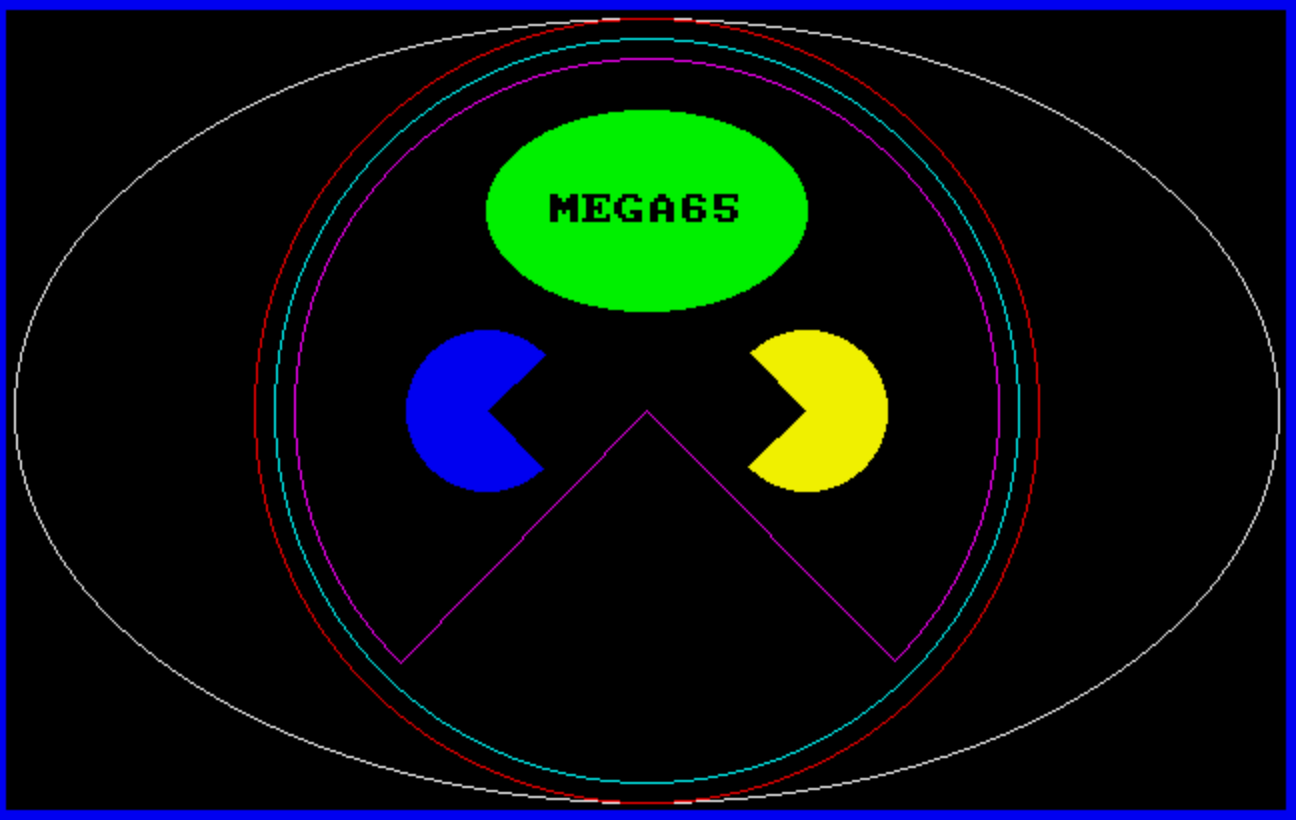
\includegraphics[width=\linewidth]{images/ellipse.png}

\newpage
\begin{tcolorbox}[colback=black,coltext=white]
\verbatimfont{\codefont}
\begin{verbatim}
100 REM ELLIPSE
110 S%=0                        :REM SCREEN
120 W%=0                        :REM WIDTH  320
130 H%=0                        :REM HEIGHT 200
140 B%=2                        :REM BITPLANES
150 POKE 0,65                   :REM 40 MEGAHERTZ
160 W=(W%+1)*320:H=(H%+1)*200   :REM WIDTH & HEIGHT IN PIXELS
170 X0=W/2:Y0=H/2:XD=W/4:YD=H/4 :REM CENTRE AND HALF AXIS
180 BORDER 0                    :REM BLACK
190 BACKGROUND 0                :REM BLACK
200 FOREGROUND 5                :REM GREEN
210 GRAPHIC CLR                 :REM INIT
220 SCREEN DEF S%,W%,H%,B%      :REM SET PARAMETERS
230 SCREEN OPEN S%              :REM OPEN
240 SCREEN SET S%,S%            :REM SET VIEW AND DRAW SCREEN
250 SCNCLR S%                   :REM CLEAR SCREEN
260 PALETTE S%,0, 0, 0, 0       :REM BLACK
270 PALETTE S%,1,15,15,15       :REM WHITE
280 PALETTE S%,2,15, 0, 0       :REM RED
290 PALETTE S%,3, 0, 0,15       :REM BLUE
300 PEN 0,2                     :REM DRAW PEN
310 ELLIPSE X0,Y0,XD,YD,1
320 PEN 0,3                     :REM DRAW PEN
330 ELLIPSE X0,Y0,XD+8,YD+8,0
340 A$=STR$(W)+" X"+STR$(H)+" X"+STR$(B%)
350 PEN 0,1                     :REM DRAW PEN
360 CHAR  12,10,1,1,2,A$
370 GETKEY A$
380 SCREEN CLOSE S%
390 PALETTE RESTORE
\end{verbatim}
\end{tcolorbox}
\end{description}
% ****
% ELSE
% ****

\newpage
\subsection{ELSE}
\index{ELSE}
\index{BASIC 65 Commands!ELSE}
\begin{description}[leftmargin=2cm,style=nextline]
\item [Token:] \$D5
\item [Format:] {\bf IF expression THEN true clause ELSE false clause}
\item [Usage:] The {\bf ELSE} keyword is part of an {\bf IF}
               statement.

               {\bf expression} is a logical or numeric expression.
               A numerical expression is evaluated as {\bf FALSE}
               if the value is zero and {\bf TRUE} for any non zero
               value.

               {\bf true clause} are one or more statements starting
               directly after {\bf THEN} on the same line.
               A linenumber after {\bf THEN} performs a
               {\bf GOTO} to that line.

               {\bf false clause} are one or more statements starting
               directly after {\bf ELSE} on the same line.
               A linenumber after {\bf ELSE} performs a
               {\bf GOTO} to that line.

\item [Remarks:]
               The standard {\bf IF ... THEN ... ELSE} structure
               is restricted to a single line. But the {\bf true clause}
               or {\bf false clause} may be expanded to several lines
               using a compound statement bracketed with the keywords
               {\bf BEGIN} and {\bf BEND}.
\item [Example:]
                Using {\bf ELSE}
\begin{tcolorbox}[colback=black,coltext=white]
\verbatimfont{\codefont}
\begin{verbatim}
100 REM ELSE
110 RED$=CHR$(28):BLACK$=CHR$(144):WHITE$=CHR$(5)
120 INPUT "ENTER A NUMBER";V
130 IF V<0 THENPRINT RED$;:ELSEPRINT BLACK$;
140 PRINT V : REM PRINT NEGATIVE NUMBERS IN RED
150 PRINT WHITE$
160 INPUT "END PROGRAM:(Y/N)";A$
170 IF A$="Y" THENEND
180 IF A$="N" THEN120:ELSE160
\end{verbatim}
\end{tcolorbox}
\end{description}


% ***
% END
% ***

\newpage
\subsection{END}
\index{END}
\index{BASIC 65 Commands!END}
\begin{description}[leftmargin=2cm,style=nextline]
\item [Token:] \$80
\item [Format:] {\bf END}
\item [Usage:] Ends the execution
               of the BASIC program. The {\bf READY.} prompt
               appears and the computer goes into direct mode
               waiting for keyboard input.

\item [Remarks:]
               {\bf END} does {\bf not} clear channels or close files.
               Also variable definitions are still valid after {\bf END}.
               The program may be continued with the {\bf CONT}
               statement. After executing the very last line of the
               program {\bf END} is executed automatically.


\item [Example:]
                Using {\bf END}
\begin{tcolorbox}[colback=black,coltext=white]
\verbatimfont{\codefont}
\begin{verbatim}
10 IF V < 0 THEN END : REM NEGATIVE NUMBERS END THE PROGRAM
20 PRINT V
\end{verbatim}
\end{tcolorbox}
\end{description}

% ********
% ENVELOPE
% ********

\newpage
\subsection{ENVELOPE}
\index{ENVELOPE}
\index{BASIC 65 Commands!ENVELOPE}
\begin{description}[leftmargin=2cm,style=nextline]
\item [Token:] \$FE \$0A
\item [Format:] {\bf ENVELOPE n, [attack,decay,sustain,release,
                waveform,pw]}
\item [Usage:] Used to define
               the parameters for the synthesis of a musical
               instrument.

      {\bf n} = envelope slot (0 -> 9)

      {\bf attack} = attack rate (0 -> 15)

      {\bf decay} = decay rate (0 -> 15)

      {\bf sustain} = sustain rate (0 -> 15)

      {\bf release} = release rate (0 -> 15)

      {\bf waveform} = (0:triangle, 1:sawtooth, 2:square/pulse, 3:noise,
                       4:ring modulation)

      {\bf pw} = pulse width (0 -> 4095) for waveform = pulse.

               There are 10 slots for storing tunes,
               preset with following values:

\ttfamily
{\setlength{\tabcolsep}{1mm}
\begin{tabular}{*{6}{|R{5mm}}|R{9mm}|l|}
\hline
 n  & A & D  & S  & R  & WF & PW     & Instrument \\
\hline
  0 & 0 &  9 &  0 &  0 &  2 &  1536  &     piano \\
  1 & 12&  0 & 12 &  0 &  1 &        &     accordion \\
  2 & 0 &  0 & 15 &  0 &  0 &        &     calliope \\
  3 & 0 &  5 &  5 &  0 &  3 &        &     drum \\
  4 & 9 &  4 &  4 &  0 &  0 &        &     flute \\
  5 & 0 &  9 &  2 &  1 &  1 &        &     guitar \\
  6 & 0 &  9 &  0 &  0 &  2 &  512   &     harpsichord \\
  7 & 0 &  9 &  9 &  0 &  2 &  2048  &     organ \\
  8 & 8 &  9 &  4 &  1 &  2 &  512   &     trumpet \\
  9 & 0 &  9 &  0 &  0 &  0 &        &     xylophone \\
\hline
\end{tabular}
}
\item [Example:]
                Using {\bf ENVELOPE}
\begin{tcolorbox}[colback=black,coltext=white]
\verbatimfont{\codefont}
\begin{verbatim}
10 ENVELOPE 9,10,5,10,5,2,4000:PLAY "T9"
20 VOL 8
30 TEMPO 100
40 PLAY "C D E F G A B"
50 PLAY "U5 V1 C D E F G A B"
\end{verbatim}
\end{tcolorbox}
\end{description}

% *****
% ERASE
% *****

\newpage
\subsection{ERASE}
\index{ERASE}
\index{BASIC 65 Commands!ERASE}
\begin{description}[leftmargin=2cm,style=nextline]
\item [Token:] \$FE \$2A
\item [Format:] {\bf ERASE filename [,D drive] [,U unit] [,R]}
\item [Usage:] Used
               to erase a disk file.

   \filenamedefinition

   \drivedefinition

   \unitdefinition

   {\bf R} = Recover a previously erased file.
   This will only work, if there were no write operations
   between erasing and recovery, which may have altered the
   contents of the file.

\item [Remarks:] The {\bf ERASE filename} command works like the
                 {\bf SCRATCH filename} command.

                 The success and the number of erased files can
                 be examined by printing or using the system
                 variable DS\$. The second last number, which
                 reports the track number in case of an disk error,
                 now reports the number of successfully erased files.

\item [Example:] Using {\bf ERASE}
\begin{tcolorbox}[colback=black,coltext=white]
\verbatimfont{\codefont}
\begin{verbatim}
  SCRATCH "DRM",U9 :REM SCRATCH FILE DRM ON UNIT 9
  PRINT DS$
  01, FILES SCRATCHED,01,00
  SCRATCH "OLD*"   :REM SCRATCH ALL FILES BEGINNING WITH "OLD"
  PRINT DS$
  01, FILES SCRATCHED,04,00
\end{verbatim}
\end{tcolorbox}
\end{description}

% **
% ER
% **

\newpage
\subsection{ER}
\index{ER}
\index{BASIC 65 System Variables!ER}
\begin{description}[leftmargin=2cm,style=nextline]
\item [Format:] {\bf ER} is a reserved system variable
\item [Usage:]  {\bf ER} has the value of the latest BASIC error
               occurred or the value -1 if there was no error.

This variable is typically used in a TRAP routine,
where the error number is taken from {\bf ER}.

\item [Example:] Using {\bf ER}
\begin{tcolorbox}[colback=black,coltext=white]
\verbatimfont{\codefont}
\begin{verbatim}
10 TRAP 100

100 IF ER>0 AND ER<42 THEN PRINT ERR$(ER);" ERROR"
110 RESUME
\end{verbatim}
\end{tcolorbox}
\end{description}

% *****
% ERR\$
% *****

\newpage
\subsection{ERR\$}
\index{ERR\$}
\index{BASIC 65 Functions!ERR\$}
\begin{description}[leftmargin=2cm,style=nextline]
\item [Token:] \$D3
\item [Format:] {\bf ERR\$(number)}
\item [Usage:] Used to convert
               an error number to an error string.

   {\bf number} is a BASIC error number (1 -> 41).

This function is typically used in a TRAP routine,
where the error number is taken from the reserved variable {\bf ER}.

\item [Remarks:] Arguments out of range (1 -> 41) will
                 produce an 'ILLEGAL QUANTITY' error.

\item [Example:] Using {\bf ERR\$}
\begin{tcolorbox}[colback=black,coltext=white]
\verbatimfont{\codefont}
\begin{verbatim}
10 TRAP 100

100 IF ER>0 AND ER<42 THEN PRINT ERR$(ER);" ERROR"
110 RESUME
\end{verbatim}
\end{tcolorbox}
\end{description}

% ****
% EXIT
% ****

\newpage
\subsection{EXIT}
\index{EXIT}
\index{BASIC 65 Commands!EXIT}
\begin{description}[leftmargin=2cm,style=nextline]
\item [Token:] \$FD
\item [Format:] {\bf EXIT}
\item [Usage:] Exits the current {\bf DO .. LOOP}
               and continues execution at the first
               statement after the next {\bf LOOP} statement.

\item [Remarks:] In nested loops {\bf EXIT} exits only one loop
               continuing executing in the next outer loop
               if there is one.
\item [Example:] Using {\bf EXIT}
\begin{tcolorbox}[colback=black,coltext=white]
\verbatimfont{\codefont}
\begin{verbatim}
1 REM EXIT
10 OPEN 2,8,0,"$"            : REM OPEN CATALOG
15 IF DS THEN PRINT DS$: STOP: REM CANT READ
20 GET#2,D$,D$               : REM DISCARD LOAD ADDRESS
25 DO                        : REM LINE LOOP
30   GET#2,D$,D$             : REM DISCARD LINE LINK
35   IF ST THEN EXIT         : REM END-OF-FILE
40   GET#2,LO,HI             : REM FILE SIZE BYTES
45   S=LO + 256 * HI         : REM FILE SIZE
50   LINE INPUT#2, F$        : REM FILE NAME
55   PRINT S;F$              : REM PRINT FILE ENTRY
60 LOOP
65 CLOSE 2
\end{verbatim}
\end{tcolorbox}
\end{description}

% ***
% EXP
% ***

\newpage
\subsection{EXP}
\index{EXP}
\index{BASIC 65 Functions!EXP}
\begin{description}[leftmargin=2cm,style=nextline]
\item [Token:] \$BD
\item [Format:] {\bf EXP(numeric expression)}
\item [Usage:] The {\bf EXP} (EXPonential function) computes
               the value of the mathematical constant
               Euler's number {\bf e = 2.71828183}
               raised to the power of the
               argument.

\item [Remarks:] An argument greater than 88 produces
                 an OVERFLOW ERROR:
\item [Example:] Using {\bf EXP}
\begin{tcolorbox}[colback=black,coltext=white]
\verbatimfont{\codefont}
\begin{verbatim}
PRINT EXP(1)
 2.71828183

PRINT EXP(0)
 1

PRINT EXP(LOG(2))
 2
\end{verbatim}
\end{tcolorbox}
\end{description}

% ****
% FAST
% ****

\newpage
\subsection{FAST}
\index{FAST}
\index{BASIC 65 Commands!FAST}
\begin{description}[leftmargin=2cm,style=nextline]
\item [Token:] \$FE \$25
\item [Format:] {\bf FAST}
\item [Usage:] Sets the system speed to 3.5 MHz.
               The system default is {\bf FAST}.
               However after using {\bf SLOW}, {\bf FAST} can be used to return
               to fast mode.

\item [Remarks:] Switching the MEGA65 to the fastest mode at 40 MHz
                 is done with the command {\bf POKE 0,65}.

\item [Example:] Using {\bf FAST}
\begin{tcolorbox}[colback=black,coltext=white]
\verbatimfont{\codefont}
\begin{verbatim}
10 SLOW
20 GOSUB 1000:REM DO SOME SLOW I/O
30 FAST
\end{verbatim}
\end{tcolorbox}
\end{description}

% ******
% FILTER
% ******

\newpage
\subsection{FILTER}
\index{FILTER}
\index{BASIC 65 Commands!FILTER}
\begin{description}[leftmargin=2cm,style=nextline]
\item [Token:] \$FE \$03
\item [Format:] {\bf FILTER [freq, lp, bp, hp, res]}
\item [Usage:] Sets
               the parameters for sound filter.

      {\bf freq} = filter cut off frequency (0 -> 2047)

      {\bf lp} = low pass filter (0:off, 1:on)

      {\bf bp} = band pass filter (0:off, 1:on)

      {\bf hp} = high pass filter (0:off, 1:on)

      {\bf resonance} = resonance (0 -> 15)

\item [Remarks:] Missing parameter keep their current value.
                 The effective filter is the sum of
                 of all filter settings.
                 This enables band reject and notch effects.

\item [Example:]
                Using {\bf FILTER}
\begin{tcolorbox}[colback=black,coltext=white]
\verbatimfont{\codefont}
\begin{verbatim}
FILTER 1023,1,0,0,10 :REM LOW PASS
FILTER 1023,0,1,0,10 :REM BAND PASS
FILTER 1023,0,0,1,10 :REM HIGH PASS
\end{verbatim}
\end{tcolorbox}
\end{description}

% ****
% FIND
% ****

\newpage
\subsection{FIND}
\index{FIND}
\index{BASIC 65 Commands!FIND}
\begin{description}[leftmargin=2cm,style=nextline]
\item [Token:] \$FE \$2B
\item [Format:] {\bf FIND {\bf delimiter} string {\bf delimiter} [,from-to]}
\item [Usage:]  {\bf FIND} is an editor command and can be used
                in direct mode only. It searches the line range
                (if specified) or the whole BASIC program else.
                At each occurrence of the "find string" the line is
                listed with the string highlighted.
                The <NO-SCROLL> key can be used to pause the output.

\item [Remarks:] Basically any unshifted character, that is not part of
                 the string, can be used as delimiter.

                 But using quotes {\bf "} as delimiter has a special effect:
                 In this case the search text is not tokenised:
                 FIND "FOR" will search the three letters F, O, R, not
                 the BSASIC keyword {\bf FOR}. So it can find the word
                 {\bf FOR} in string constants or REM statements, but not
                 in program code.

                 On the other hand FIND /FOR/ will find all occurences of
                 the BASIC keyword, but not the text "FOR" in strings.

                 Also notice, that you cannot search for partial keywords.
                 {\bf FIND /LOO/} will not find the keyword {\bf LOOP},


\item [Example:] Using {\bf FIND}
\end{description}
\begin{center}
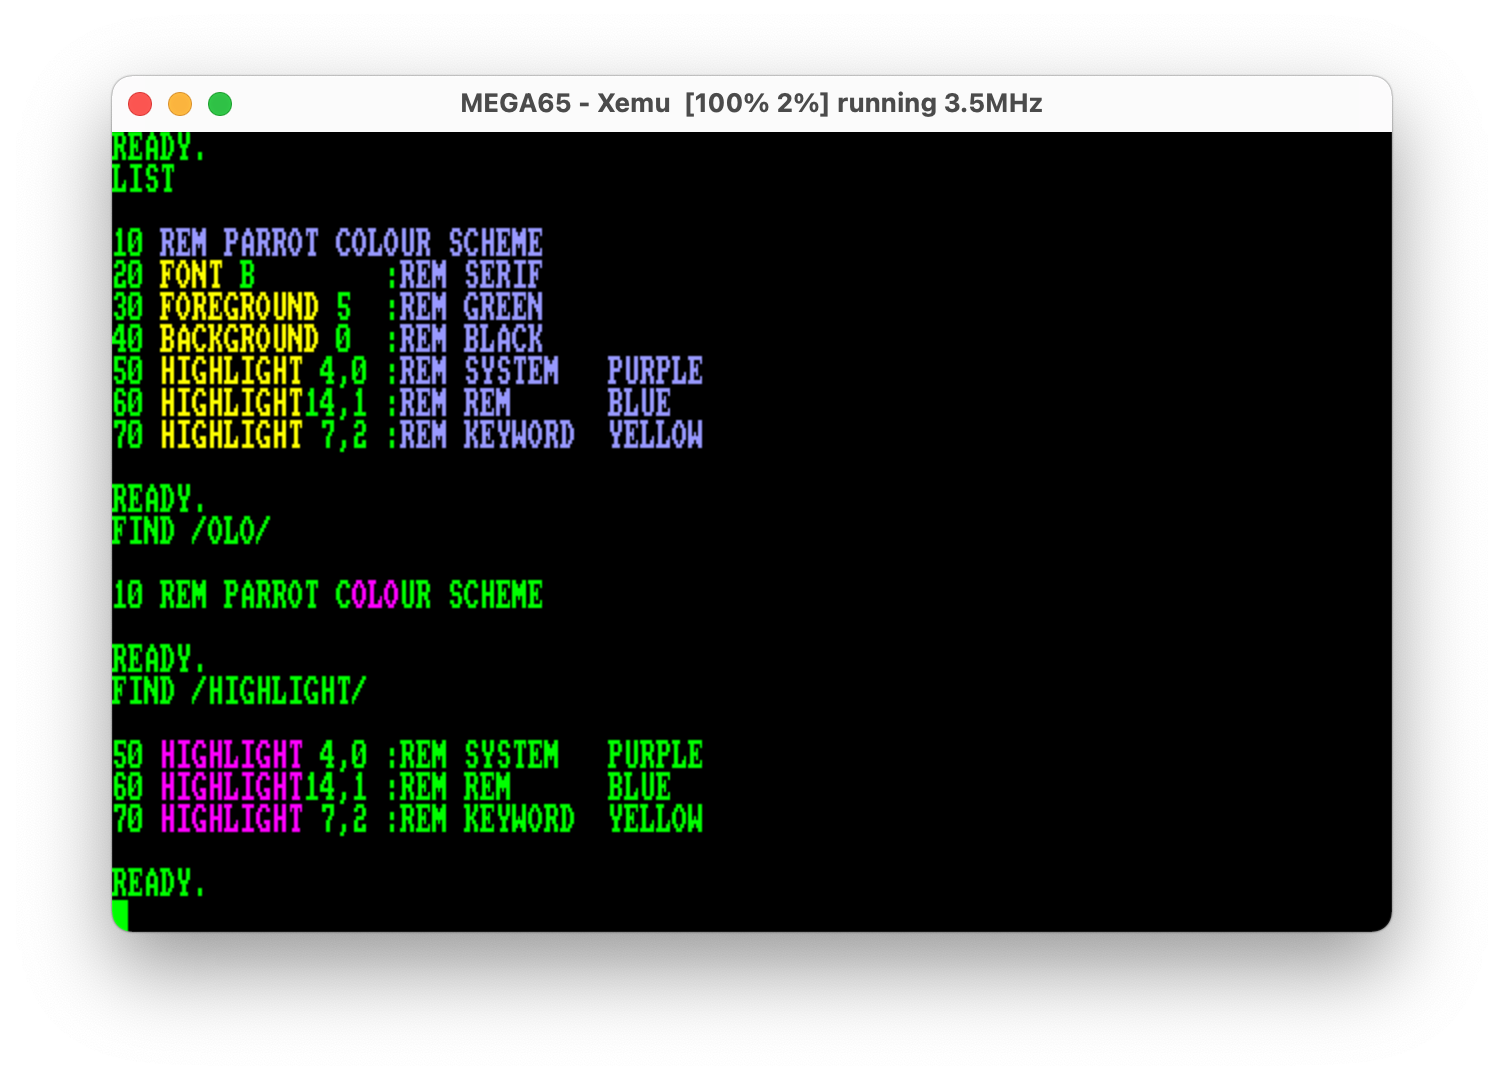
\includegraphics[width=0.8\linewidth]{images/highlight.png}
\end{center}

% **
% FN
% **

\newpage
\subsection{FN}
\index{FN}
\index{BASIC 65 Functions!FN}
\begin{description}[leftmargin=2cm,style=nextline]
\item [Token:] \$A5
\item [Format:] {\bf FN name(numeric expression)}
\item [Usage:] The {\bf FN} functions are user defined
               functions, that accept a numeric expression as
               argument and return a real value.
               They must be defined with {\bf DEF FN} before
               the first usage.

\item [Example:] Using {\bf FN}
\begin{tcolorbox}[colback=black,coltext=white]
\verbatimfont{\codefont}
\begin{verbatim}
10 PD = ~ / 180
20 DEF FN CD(X)= COS(X*PD): REM COS FOR DEGREES
30 DEF FN SD(X)= SIN(X*PD): REM SIN FOR DEGREES
40 FOR D=0 TO 360 STEP 90
50 PRINT USING "###";D
60 PRINT USING " ##.##";FNCD(D);
70 PRINT USING " ##.##";FNSD(D)
80 NEXT D
RUN
  0  1.00  0.00
 90  0.00  1.00
180 -1.00  0.00
270  0.00 -1.00
360  1.00  0.00
\end{verbatim}
\end{tcolorbox}
\end{description}

% ****
% FONT
% ****

\newpage
\subsection{FONT}
\index{FONT}
\index{BASIC 65 Commands!FONT}
\begin{description}[leftmargin=2cm,style=nextline]
\item [Token:] \$FE \$46
\item [Format:] {\bf FONT [A|B|C]}
\item [Usage:] The {\bf FONT} command is used to switch between fonts
               and the code pages PETSCII and enhanced PETSCII.
               The enhanced PETSCII includes all ASCII symbols, that
               are missing in the PETSCII code page, though the order
               is still PETSCII.
               The ASCII symbols are typed by holding the \megasymbolkey
               together with the desired key.
               The codes for uppercase and lowercase
               are swapped compared to ASCII.
               The uppercase/graphics code page is not changed.

\ttfamily
{\setlength{\tabcolsep}{1mm}
\begin{tabular}{*{4}{|R{2.0cm}}|}
\hline
 code  &   key & PETSCII & ASCII  \\
\hline
\$5C & pound      & {\codefont \textbackslash}   & \textbackslash  \\
\$5E & up arrow   & {\codefont \textasciicircum} & \textasciicircum  \\
\$5F & back arrow & {\codefont \_}               & \_   \\
\$7B & colon      & {\codefont ě }               & \{   \\
\$7C & dot        & {\codefont Ĝ }               &  |   \\
\$7D & semicolon  & {\codefont ĝ }               & \}   \\
\$7E & comma      & {\codefont \textasciitilde}  & \textasciitilde   \\
\hline
\end{tabular}
}

% \verbatimfont{\codefont}
% \begin{verbatim}
%  !"#$%&'()*+,-./    20
% 0123456789:;<=>?    30
% @ABCDEFGHIJKLMNO    40
% PQRSTUVWXYZ[\]^_    50
% `abcdefghijklmno    60
% pqrstuvwxyz{|}~     70
%
% ÀÁÂÃÄÅÆÇÈÉÊËÌÍÎÏ  c380
% ÐÑÒÓÔÕÖ×ØÙÚÛÜÝÞß  c390
% àáâãäåæçèéêëìíîï  c3a0
% ðñòóôõö÷øùúûüýþÿ  c3b0
%
% ĀāĂ㥹ĆćĈĉĊċČčĎď  c480
% ĐđĒēĔĕĖėĘęĚěĜĝĞğ  c490
% ĠġĢģĤĥĦħĨĩĪīĬĭĮį  c4a0
% İıIJijĴĵĶķĸĹĺĻļĽľĿ  c4b0
% ŀŁłŃńŅņŇňʼnŊŋŌōŎŏ  c580
% ŐőŒœŔŕŖŗŘřŚśŜŝŞş  c590
%
% ŠšŢţŤťŦŧŨũŪūŬŭŮů  c5a0
% ŰűŲųŴŵŶŷŸŹźŻżŽžſ  c5b0
% ƀƁƂƃƄƅƆƇƈƉƊƋƌƍƎƏ  c680
% ƐƑƒƓƔƕƖƗƘƙƚƛƜƝƞƟ  c690
% \end{verbatim}


\item [Example:] Using {\bf FONT}
\begin{tcolorbox}[colback=black,coltext=white]
%\verbatimfont{\codefont}
\begin{verbatim}
FONT A :REM ASCII - ENABLE {|}_~^
FONT B :REM LIKE A, WITH A SERIF FONT
FONT C :REM COMMODORE FONT (DEFAULT)
\end{verbatim}
\end{tcolorbox}
\end{description}

% ***
% FOR
% ***

\newpage
\subsection{FOR}
\index{FOR}
\index{BASIC 65 Commands!FOR}
\begin{description}[leftmargin=2cm,style=nextline]
\item [Token:] \$81
\item [Format:] {\bf FOR index=start TO end [STEP step] ... NEXT [index]}
\item [Usage:] The {\bf FOR} statement starts the definition
               of a BASIC loop with an index variable.

               The {\bf index} variable may be incremented or decremented
               by a constant value on each iteration. The default
               is to increment the variable by 1.
               The index variable must be a real variable.

               The {\bf start} value is used to initialise the index.

               The {\bf end} value is used at the end of the loop
               and controls, whether the next iteration will be started
               or the loop exited.

               The {\bf step} value defines the change applied to
               to the index variable at the end of the loop.
               Positive step values increment it, while negative values
               decrement it. It defaults to 1.0 if not specified.

\item [Remarks:] For positive increments {\bf end} must be greater
               or equal than {\bf start}, for negative increments
               {\bf end} must be less or equal than {\bf start}.

               It is bad programming style to change the value
               of the index variable inside the loop or to
               jump into or out of the loop body with {\bf GOTO}.

\item [Example:] Using {\bf FOR}
\begin{tcolorbox}[colback=black,coltext=white]
\verbatimfont{\codefont}
\begin{verbatim}
10 FOR D=0 TO 360 STEP 30
20 R = D * ~ / 180
30 PRINT D;R;SIN(R);COS(R);TAN(R)
40 NEXT D

10 DIM M(20,20)
20 FOR I=0 TO 20
30 FOR J=I TO 20
40 M(I,J) = I + 100 * J
50 NEXT J,I
\end{verbatim}
\end{tcolorbox}
\end{description}

% **********
% FOREGROUND
% **********

\newpage
\subsection{FOREGROUND}
\index{FOREGROUND}
\index{BASIC 65 Commands!FOREGROUND}
\begin{description}[leftmargin=2cm,style=nextline]
\item [Token:] \$FE \$39
\item [Format:] {\bf FOREGROUND colour}
\item [Usage:] Sets the foreground colour
               (text colour) of the screen to the argument,
               which must be in the
               range 0 to 15. (See colour table).
\item [Example:] \screentext{FOREGROUND  7} - select foreground colour yellow.
\item [Colours:] {\bf Index and RGB values of colour palette}

\ttfamily
{\setlength{\tabcolsep}{1mm}
\begin{tabular}{*{4}{|R{1.2cm}}|l|}
\hline
 index  &   red & green & blue & colour \\
\hline
  0 &    0  &   0   &  0   & black \\
  1 &   15  &  15   & 15   & white \\
  2 &   15  &   0   &  0   & red   \\
  3 &    0  &  15   & 15   & cyan  \\
  4 &   15  &   0   & 15   & magenta\\
  5 &    0  &  15   &  0   & green \\
  6 &    0  &   0   & 15   & blue  \\
  7 &   15  &  15   &  0   & yellow\\
  8 &   15  &   6   &  0   & orange\\
  9 &   10  &   4   &  0   & brown \\
 10 &   15  &   7   &  7   & pink  \\
 11 &    5  &   5   &  5   & dark grey\\
 12 &    8  &   8   &  8   & medium grey\\
 13 &    9  &  15   &  9   & light green \\
 14 &    9  &   9   & 15   & light blue\\
 15 &   11  &  11   & 11   & light grey\\
\hline
\end{tabular}
}
\end{description}

% ***
% FRE
% ***

\newpage
\subsection{FRE}
\index{FRE}
\index{BASIC 65 Functions!FRE}
\begin{description}[leftmargin=2cm,style=nextline]
\item [Token:] \$B8
\item [Format:] {\bf FRE(bank)}
\item [Usage:] Returns the number of free bytes for banks 0 or 1,
               or the ROM version, if the argument is negative.

               {\bf FRE(0)} returns the number of free bytes in
               bank 0, which is used for BASIC program source.

               {\bf FRE(1)} returns the number of free bytes in
               bank 1, which is the bank for BASIC variables, arrays
               and strings. A usage of {\bf FRE(1)} also triggers the
               "garbage collection", a process, that collects
               used strings at the top of the bank, thereby
               defragmenting string memory.

               {\bf FRE(-1)} returns the ROM version, a six-digit number
               of the form 92xxxx.

\item [Example:] Using {\bf FRE}:
\begin{tcolorbox}[colback=black,coltext=white]
\verbatimfont{\codefont}
\begin{verbatim}
10 PM = FRE(0)
20 VM = FRE(1)
30 RV = FRE(-1)
40 PRINT PM;" FREE FOR PROGRAM"
50 PRINT VM;" FREE FOR VARIABLES"
60 PRINT RV;" ROM VERSION"
\end{verbatim}
\end{tcolorbox}
\end{description}

% *****
% FREAD
% *****

\newpage
\subsection{FREAD}
\index{FREAD}
\index{BASIC 65 Functions!FREAD}
\begin{description}[leftmargin=2cm,style=nextline]
\item [Token:] \$FE \$1C
\item [Format:] {\bf FREAD\#channel, pointer, size}
\item [Usage:] Reads {\bf size} bytes from {\bf channel} to memory
               starting at the 32 bit address {\bf pointer}.

               Care must be taken, not to overwrite memory,
               that is used by the system or the interpreter.

               It is recommended to use the {\bf POINTER} statement
               for the pointer argument and compute the size parameter
               by multiplying the number of elements with the item size.

{\ttfamily
\setlength{\tabcolsep}{1mm}
\begin{tabular}{|l|l|}
\hline
 type          & item size \\
\hline
byte     array &  1     \\
integer  array &  2     \\
real     array &  5     \\
\hline
\end{tabular}
}

Keep in mind, that the {\bf POINTER} function with a string argument
does NOT return the string address, but the string descriptor.
It is recommend, not to use {\bf FREAD} for strings or string arrays
unless you are fully aware, how to handle the string storage internals.

Also take care, that you always specify an index, if you use an array.
The start address of array XY() is POINTER(XY(0)).
POINTER(XY) returns the address of the scalar variable XY.

\item [Example:] Using {\bf FREAD}:
\begin{tcolorbox}[colback=black,coltext=white]
\verbatimfont{\codefont}
\begin{verbatim}
100 N=23
110 DIM B&(N),C&(N)
120 DOPEN#2,"TEXT"
130 FREAD#2,POINTER(B&(0)),N
140 DCLOSE#2
150 FORI=0TON-1:PRINTCHR$(B&(I));:NEXT
160 FORI=0TON-1:C&(I)=B&(N-1-I):NEXT
170 DOPEN#2,"REVERS",W
180 FWRITE#2,POINTER(C&(0)),N
190 DCLOSE#2
\end{verbatim}
\end{tcolorbox}
\end{description}

% *****
% FWRITE
% *****

\newpage
\subsection{FWRITE}
\index{FWRITE}
\index{BASIC 65 Functions!FWRITE}
\begin{description}[leftmargin=2cm,style=nextline]
\item [Token:] \$FE \$1E
\item [Format:] {\bf FWRITE\#channel, pointer, size}
\item [Usage:] Writes {\bf size} bytes from {\bf channel} to memory
               starting at the 32 bit address {\bf pointer}.

               It is recommended to use the {\bf POINTER} statement
               for the pointer argument and compute the size parameter
               by multiplying the number of elements with the item size.

{\ttfamily
\setlength{\tabcolsep}{1mm}
\begin{tabular}{|l|l|}
\hline
 type          & item size \\
\hline
byte     array &  1     \\
integer  array &  2     \\
real     array &  5     \\
\hline
\end{tabular}
}

Keep in mind, that the {\bf POINTER} function with a string argument
does NOT return the string address, but the string descriptor.
It is recommend, not to use {\bf FWRITE} for strings or string arrays
unless you are fully aware, how to handle the string storage internals.

Also take care, that you always specify an index, if you use an array.
The start address of array XY() is POINTER(XY(0)).
POINTER(XY) returns the address of the scalar variable XY.

\item [Example:] Using {\bf FWRITE}:
\begin{tcolorbox}[colback=black,coltext=white]
\verbatimfont{\codefont}
\begin{verbatim}
100 N=23
110 DIM B&(N),C&(N)
120 DOPEN#2,"TEXT"
130 FREAD#2,POINTER(B&(0)),N
140 DCLOSE#2
150 FORI=0TON-1:PRINTCHR$(B&(I));:NEXT
160 FORI=0TON-1:C&(I)=B&(N-1-I):NEXT
170 DOPEN#2,"REVERS",W
180 FWRITE#2,POINTER(C&(0)),N
190 DCLOSE#2
\end{verbatim}
\end{tcolorbox}
\end{description}

% ***
% GET
% ***

\newpage
\subsection{GET}
\index{GET}
\index{BASIC 65 Commands!GET}
\begin{description}[leftmargin=2cm,style=nextline]
\item [Token:] \$A1
\item [Format:] {\bf GET variable}
\item [Usage:] Gets the next character or byte value of that character
               from the keyboard queue.
               If the variables is of type string and the queue is empty
               an empty string is assigned to the variable,
               otherwise a one character string is created
               and assigned to the string variable.
               If the variable is of numeric type, the character code
               of the key is assigned to it, or zero if there was no keypress.
               This command does not wait for keyboard
               input, so it's useful to check for key presses
               in regular intervals or loops.

\item [Remarks:] The command {\bf GETKEY} is similar, but waits
                 until a key was hit.

\item [Example:] Using {\bf GET}:
\begin{tcolorbox}[colback=black,coltext=white]
\verbatimfont{\codefont}
\begin{verbatim}
10 DO: GET A$: LOOP UNTIL A$ <> ""
40 IF A$ = "W" THEN 1000 :REM GO NORTH
50 IF A$ = "A" THEN 2000 :REM GO WEST
60 IF A$ = "S" THEN 3000 :REM GO EAST
70 IF A$ = "Z" THEN 4000 :REM GO SOUTH
80 IF A$ = CHR$(13) THEN 5000 :REM RETURN
90 GOTO 10
\end{verbatim}
\end{tcolorbox}
\end{description}

% ****
% GET#
% ****

\newpage
\subsection{GET\#}
\index{GET\#}
\index{BASIC 65 Commands!GET\#}
\begin{description}[leftmargin=2cm,style=nextline]
\item [Token:] \$A1 '\#'
\item [Format:] {\bf GET\# channel, list of variables}
\item [Usage:] Reads as many bytes
               as necessary from the channel argument
               and assigns strings of length one to
               string variables or the read 8-bit binary value
               to numeric variables.
               This is useful to read characters or bytes from
               an input stream one by one.

\item [Remarks:] All values from 0 to 255 are valid, so this
               command can also be used to read binary data.

\item [Example:] Using {\bf GET\#} to read a disk directory:
\begin{tcolorbox}[colback=black,coltext=white]
\verbatimfont{\codefont}
\begin{verbatim}
1 REM GET#
10 OPEN 2,8,0,"$"            : REM OPEN CATALOG
15 IF DS THEN PRINT DS$: STOP: REM CANT READ
20 GET#2,D$,D$               : REM DISCARD LOAD ADDRESS
25 DO                        : REM LINE LOOP
30   GET#2,D$,D$             : REM DISCARD LINE LINK
35   IF ST THEN EXIT         : REM END-OF-FILE
40   GET#2,LO,HI             : REM FILE SIZE BYTES
45   S=LO + 256 * HI         : REM FILE SIZE
50   LINE INPUT#2, F$        : REM FILE NAME
55   PRINT S;F$              : REM PRINT FILE ENTRY
60 LOOP
65 CLOSE 2
\end{verbatim}
\end{tcolorbox}
\end{description}

% ******
% GETKEY
% ******

\newpage
\subsection{GETKEY}
\index{GETKEY}
\index{BASIC 65 Commands!GETKEY}
\begin{description}[leftmargin=2cm,style=nextline]
\item [Token:] \$A1 \$F9 (GET token and KEY token)
\item [Format:] {\bf GETKEY variable}
\item [Usage:] Gets the next character or code value
               from the keyboard queue. If the queue is empty
               the program waits until a key is hit.
               Then a one character string is created
               and assigned to the string variable.
               If the variable is numeric, the character code
               is assigned as value.

\item [Example:] Using {\bf GETKEY}:
\begin{tcolorbox}[colback=black,coltext=white]
\verbatimfont{\codefont}
\begin{verbatim}
10 GETKEY A$ :REM WAIT AND GET CHARACTER
40 IF A$ = "W" THEN 1000 :REM GO NORTH
50 IF A$ = "A" THEN 2000 :REM GO WEST
60 IF A$ = "S" THEN 3000 :REM GO EAST
70 IF A$ = "Z" THEN 4000 :REM GO SOUTH
80 IF A$ = CHR$(13) THEN 5000 :REM RETURN
90 GOTO 10
\end{verbatim}
\end{tcolorbox}
\end{description}

% ****
% GO64
% ****

\newpage
\subsection{GO64}
\index{GO64}
\index{BASIC 65 Commands!GO64}
\begin{description}[leftmargin=2cm,style=nextline]
\item [Token:] \$CB \$36 \$34 (GO token and 64 )
\item [Format:] {\bf GO64}
\item [Usage:] Switches the
               computer to the C64 compatible mode. In direct
               mode a security prompt \screentext{ARE YOU SURE?}
               is printed, which must be responded with 'Y' to
               continue. Use \screentext{SYS58552} to switch back
               to C65 mode.

\item [Example:] Using {\bf GO64}:
\begin{tcolorbox}[colback=black,coltext=white]
\verbatimfont{\codefont}
\begin{verbatim}
GO64
ARE YOU SURE?
\end{verbatim}
\end{tcolorbox}
\end{description}

% *****
% GOSUB
% *****

\newpage
\subsection{GOSUB}
\index{GOSUB}
\index{BASIC 65 Commands!GOSUB}
\begin{description}[leftmargin=2cm,style=nextline]
\item [Token:] \$8D
\item [Format:] {\bf GOSUB line}
\item [Usage:] The {\bf GOSUB} (GOto SUBroutine)
               command continues program
               execution at the given BASIC line number,
               saving the current BASIC program counter
               and line number on the run-time stack.
               This enables the resume of the execution after
               the {\bf GOSUB} statement, once a {\bf RETURN}
               statement in the called subroutine was executed.
               Calls to subroutines via {\bf GOSUB} may be nested
               but the end of the subroutine code must always
               be a {\bf RETURN}. Otherwise a stack overflow
               may occur.

\item [Remarks:] Unlike other programming languages, this BASIC
               version does not support arguments or local
               variables for subroutines. \\
               Programs can be optimised by grouping subroutines
               at the beginning of the program source. The
               {\bf GOSUB} calls will then have low line numbers
               with only few digits to decode. Also the subroutines
               will be found faster, because the search for subroutines
               starts very often at the start of the program.
\item [Example:] Using {\bf GOSUB}:
\begin{tcolorbox}[colback=black,coltext=white]
\verbatimfont{\codefont}
\begin{verbatim}
 10 GOTO 100 :REM TO MAIN PROGRAM
 20 REM *** SUBROUTINE DISK STATUS CHECK ***
 30 DD=DS:IF DD THEN PRINT "DISK ERROR";DS$
 40 RETURN
 50 REM *** SUBROUTINE PROMPT Y/N ***
 60 DO:INPUT "CONTINUE (Y/N)";A$
 70 LOOP UNTIL A$="Y" OR A$="N"
 80 RETURN
 90 REM *** MAIN PROGRAM ***
100 DOPEN#2,"BIG DATA"
110 GOSUB 30: IF DD THEN DCLOSE#2:GOSUB 60:REM ASK
120 IF A$="N" THEN STOP
130 GOTO 100: REM RETRY
\end{verbatim}
\end{tcolorbox}
\end{description}

% ****
% GOTO
% ****

\newpage
\subsection{GOTO}
\index{GOTO}
\index{BASIC 65 Commands!GOTO}
\begin{description}[leftmargin=2cm,style=nextline]
\item [Token:] \$89 (GOTO) or \$CB \$A4 (GO TO)
\item [Format:] {\bf GOTO line} \\
                {\bf GO TO line}
\item [Usage:] Continues program
               execution at the given BASIC line number.

               The {\bf GOTO} command written as a single
               word executes faster than the {\bf GO TO} command.

\item [Remarks:] The new line number will be searched by scanning
               the BASIC source linearly upwards. If the target
               line number is higher than the current one, the
               search starts from the current line upwards.
               If the target line number is lower, the search starts
               from the start of the program.
               Knowing this mechanism it is possible to optimise
               the run-time by grouping often used targets at the
               start of the program.

\item [Example:] Using {\bf GOTO}:
\begin{tcolorbox}[colback=black,coltext=white]
\verbatimfont{\codefont}
\begin{verbatim}
 10 GOTO 100 :REM TO MAIN PROGRAM
 20 REM *** SUBROUTINE DISK STATUS CHECK ***
 30 DD=DS:IF DD THEN PRINT "DISK ERROR";DS$
 40 RETURN
 50 REM *** SUBROUTINE PROMPT Y/N ***
 60 DO:INPUT "CONTINUE (Y/N)";A$
 70 LOOP UNTIL A$="Y" OR A$="N"
 80 RETURN
 90 *** MAIN PROGRAM ***
100 DOPEN#2,"BIG DATA"
110 GOTO 30: IF DD THEN DCLOSE#2:GOTO 60:REM ASK
120 IF A$="N" THEN STOP
130 GOTO 100: REM RETRY
\end{verbatim}
\end{tcolorbox}
\end{description}

% *******
% GRAPHIC
% *******

\newpage
\subsection{GRAPHIC}
\index{GRAPHIC}
\index{BASIC 65 Commands!GRAPHIC}
\begin{description}[leftmargin=2cm,style=nextline]
\item [Token:] \$DE
\item [Format:] {\bf GRAPHIC CLR}
\item [Usage:] Initialises the BASIC graphic system.
               It clears the graphics memory and screen and sets
               all parameters of the graphics context to the
               default values.

\item [Remarks:] A second form of the {\bf GRAPHIC} command,
               which serves as an interface to internal
               subroutines may be added later.

\item [Example:] Using {\bf GRAPHIC}:
\begin{tcolorbox}[colback=black,coltext=white]
\verbatimfont{\codefont}
\begin{verbatim}
100 REM GRAPHIC
110 GRAPHIC CLR        : REM INITIALISE
120 SCREEN DEF 1,1,1,2 : REM 640 X 400 X 2
130 SCREEN OPEN 1      : REM OPEN IT
140 SCREEN SET 1,1     : REM VIEW IT
150 PALETTE 1,0,0, 0,0 : REM BLACK
160 PALETTE 1,1,0,15,0 : REM GREEN
170 SCNCLR             : REM CLEAR SCREEN
180 PEN 0,1            : REM SELECT PEN
190 LINE 50,50,590,350 : REM DRAW LINE
200 GETKEY A$          : REM WAIT FOR KEYPRESS
210 SCREEN CLOSE 1     : REM CLOSE GRAPHIC SCREEN
220 PALETTE RESTORE    : REM RESTORE DEAFULT COLOURS
\end{verbatim}
\end{tcolorbox}
\end{description}

% ******
% HEADER
% ******

\newpage
\subsection{HEADER}
\index{HEADER}
\index{BASIC 65 Commands!HEADER}
\begin{description}[leftmargin=2cm,style=nextline]
\item [Token:] \$F1
\item [Format:] {\bf HEADER diskname [,Iid] [,D drive] [,U unit] }
\item [Usage:]
   Used to format or clear a diskette
   or disk.

   {\bf diskname} is either a quoted string, e.g. {\bf "data"} or
   a string expression in parentheses, e.g. {\bf (DN\$)}
   The maximum length of the diskname is 16 characters.

   \drivedefinition

   \unitdefinition

\item [Remarks:]
   For new diskettes or disks, which are not already formatted
   it is absolutely necessary to specify the disk ID with the
   parameter {\bf Iid}. This switches the format command to the
   full format, which writes sector IDs and erases all contents.
   This will need some time, because every block on the disk will
   be written. \\
   If the {\bf Iid} parameter is omitted, a quick format will
   be performed. This is only possible, if the disk is formatted
   already. A quick format writes a new disk name and clears the
   block allocation map, marking all blocks as free.
   The disk ID is not changed, the blocks are not overwritten,
   so contents may be recovered with the {\bf ERASE R} command.

\item [Example:] Using {\bf HEADER}
\begin{tcolorbox}[colback=black,coltext=white]
\verbatimfont{\codefont}
\begin{verbatim}
  HEADER "ADVENTURE",IBS
  HEADER "ZORK-I",U9
  HEADER "DUNGEON",D1,U10
\end{verbatim}
\end{tcolorbox}
\end{description}

% ****
% HELP
% ****

\newpage
\subsection{HELP}
\index{HELP}
\index{BASIC 65 Commands!HELP}
\begin{description}[leftmargin=2cm,style=nextline]
\item [Token:] \$EA
\item [Format:] {\bf HELP}
\item [Usage:]
   When the BASIC program stops due to an error, type
   {\bf HELP} for further information.
   The interpreted line is listed, with the
   erroneous statement highlighted or underlined.

\item [Remarks:]
      Displays BASIC errors. For errors in disk
      I/O one should print the disk status variable {\bf DS}
      or the disk status string {\bf DS\$}.

\item [Example:] Using {\bf HELP}
\begin{tcolorbox}[colback=black,coltext=white]
\verbatimfont{\codefont}
\begin{verbatim}
10 A=1.E20
20 B=A+A:C=EXP(A):PRINT A,B,C
RUN

?OVERFLOW ERROR IN 20
READY.
HELP

20 B=A+A:ţŝťŸŰňšʼn:PRINT A,B,C
\end{verbatim}
\end{tcolorbox}
\end{description}

% *****
% HEX\$
% *****

\newpage
\subsection{HEX\$}
\index{HEX\$}
\index{BASIC 65 Functions!HEX\$}
\begin{description}[leftmargin=2cm,style=nextline]
\item [Token:] \$D2
\item [Format:] {\bf HEX\$(numeric expression)}
\item [Usage:] Returns a four
               character string in hexadecimal notation
               converted from the argument.
               The argument must be in the range 0 -> 65535
               corresponding to the hex numbers 0000 -> FFFF.

\item [Remarks:] If real numbers are used as arguments, the
                 fractional part will be cut off, not rounded.

\item [Example:] Using {\bf HEX\$}:
\begin{tcolorbox}[colback=black,coltext=white]
\verbatimfont{\codefont}
\begin{verbatim}
PRINT HEX$(10),HEX$(100),HEX$(1000.9)
000A      0064      03E8
\end{verbatim}
\end{tcolorbox}
\end{description}

% *********
% HIGHLIGHT
% *********

\newpage
\subsection{HIGHLIGHT}
\index{HIGHLIGHT}
\index{BASIC 65 Commands!HIGHLIGHT}
\begin{description}[leftmargin=2cm,style=nextline]
\item [Token:] \$FE \$3D
\item [Format:] {\bf HIGHLIGHT colour [,mode]}
\item [Usage:] Sets the colour
               to be used for the "highlight" text attribute.
               The colour index must be in the
               range 0 to 15. (See colour table).

               The optional parameter {\bf mode} defines, how
               BASIC listings to the screen use highlighting:

{\ttfamily
\begin{tabular}{|l|l|}
\hline
   {\bf mode = 0}    &  no syntax highlighting \\
   {\bf mode = 1}    &  highlight REM statements \\
   {\bf mode = 2}    &  highlight BASIC keywords \\
\hline
\end{tabular}
}

\item [Remarks:] The highlight text attribute is used to mark text
               in listings generated by the {\bf HELP FIND CHANGE}
               commands.
\item [Example:] \screentext{HIGHLIGHT  8,2} - select highlight colour orange
                 for keywords.
\item [Colours:] {\bf Index and RGB values of colour palette}

\ttfamily
{\setlength{\tabcolsep}{1mm}
\begin{tabular}{*{4}{|R{1.2cm}}|l|}
\hline
 index  &   red & green & blue & colour \\
\hline
  0 &    0  &   0   &  0   & black \\
  1 &   15  &  15   & 15   & white \\
  2 &   15  &   0   &  0   & red   \\
  3 &    0  &  15   & 15   & cyan  \\
  4 &   15  &   0   & 15   & magenta\\
  5 &    0  &  15   &  0   & green \\
  6 &    0  &   0   & 15   & blue  \\
  7 &   15  &  15   &  0   & yellow\\
  8 &   15  &   6   &  0   & orange\\
  9 &   10  &   4   &  0   & brown \\
 10 &   15  &   7   &  7   & pink  \\
 11 &    5  &   5   &  5   & dark grey\\
 12 &    8  &   8   &  8   & medium grey\\
 13 &    9  &  15   &  9   & light green \\
 14 &    9  &   9   & 15   & light blue\\
 15 &   11  &  11   & 11   & light grey\\
\hline
\end{tabular}
}
\end{description}

% **
% IF
% **

\newpage
\subsection{IF}
\index{IF}
\index{BASIC 65 Commands!IF}
\begin{description}[leftmargin=2cm,style=nextline]
\item [Token:] \$8B
\item [Format:] {\bf IF expression THEN true clause ELSE false clause}
\item [Usage:] Starts a conditional execution
               statement.

               {\bf expression} is a logical or numeric expression.
               A numerical expression is evaluated as {\bf FALSE}
               if the value is zero and {\bf TRUE} for any non zero
               value.

               {\bf true clause} are one or more statements starting
               directly after {\bf THEN} on the same line.
               A linenumber after {\bf THEN} performs a
               {\bf GOTO} to that line.

               {\bf false clause} are one or more statements starting
               directly after {\bf ELSE} on the same line.
               A linenumber after {\bf ELSE} performs a
               {\bf GOTO} to that line.

\item [Remarks:]
               The standard {\bf IF ... THEN ... ELSE} structure
               is restricted to a single line. But the {\bf true clause}
               or {\bf false clause} may be expanded to several lines
               using a compound statement bracketed with the keywords
               {\bf BEGIN} and {\bf BEND}.
\item [Example:]
                Using {\bf IF}
\begin{tcolorbox}[colback=black,coltext=white]
\verbatimfont{\codefont}
\begin{verbatim}
10 IF V < 0 THEN PRINT RED$;:ELSE PRINT BLACK$;
20 PRINT V : REM PRINT NEGATIVE NUMBERS IN RED
30 INPUT "END PROGRAM:(Y/N)";A$
40 IF A$="Y" THEN END
50 IF A$="N" THEN 10:ELSE 30

\end{verbatim}
\end{tcolorbox}
\end{description}

% *****
% INPUT
% *****

\newpage
\subsection{INPUT}
\index{INPUT}
\index{BASIC 65 Commands!INPUT}
\begin{description}[leftmargin=2cm,style=nextline]
\item [Token:] \$85
\item [Format:] {\bf INPUT [prompt <,|;>] variable list}
\item [Usage:] Prints an optional
               prompt string and question mark to the screen,
               flashes the cursor and waits for user input
               from the keyboard.

               {\bf prompt} = string expression to be printed
               as prompt. It may be omitted. \\
               If the separator between prompt and variable list
               is a comma, the cursor is placed directly after
               the prompt. If the separator is a semicolon,
               a question mark and a space is added to the prompt.

               {\bf variable list} = list of one or more
               variables, that receive the input.

               The input will be processed after the user hits RETURN.

\item [Remarks:] The user must take care to enter the correct
               type of input matching variable types.
               Also the number of input items must match the number
               of variables.
               Entering non numeric characters for integer or real
               variables will produce a TYPE MISMATCH ERROR.
               Strings for string variables have to be put in quotes
               if they contain spaces or commas. \\
               Many programs, that need a safe input routine use
               {\bf LINE INPUT} and use an own parser, in order
               to avoid program breaks by wrong user input.

\item [Example:] Using {\bf INPUT}:
\begin{tcolorbox}[colback=black,coltext=white]
\verbatimfont{\codefont}
\begin{verbatim}
 10 DIM N$(100),A%(100),S$(100):
 20 DO
 30 INPUT "NAME, AGE, SEX";NA$,AG%,SE$
 40 IF NA$="" THEN 30
 50 IF NA$="END" THEN EXIT
 60 IF AG% < 18 OR AG% > 100 THEN PRINT "AGE?":GOTO 30
 70 IF SE$ <> "M" AND SE$ <> "F" THEN PRINT "SEX?":GOTO 30
 80 REM CHECK OK: ENTER INTO ARRAY
 90 N$(N)=NA$:A%(N)=AG%:S$(N)=SE$:N=N+1
100 LOOP UNTIL N=100
110 PRINT "RECEIVED";N;" NAMES"
\end{verbatim}
\end{tcolorbox}
\end{description}

% *******
% INPUT\#
% *******

\newpage
\subsection{INPUT\#}
\index{INPUT\#}
\index{BASIC 65 Commands!INPUT\#}
\begin{description}[leftmargin=2cm,style=nextline]
\item [Token:] \$84
\item [Format:] {\bf INPUT\# channel, variable list}
\item [Usage:] Reads a record
               from an input device, e.g. a disk file
               and assigns the data
               to the variables in the list.

               {\bf channel} = channel number assigned
               by a {\bf DOPEN} or {\bf OPEN} command.

               {\bf variable list} = list of one or more
               variables, that receive the input.

               The input record must be terminated by a
               RETURN character and must be not longer than
               the input buffer (160 characters).

\item [Remarks:] The type and number of data in a record must
               match the variable list.
               Reading non numeric characters for integer or real
               variables will produce a FILE DATA ERROR.
               Strings for string variables have to be put in quotes
               if they contain spaces or commas. \\
               The command {\bf LINE INPUT\#} may be used to
               read a whole record into a single string variable.

\item [Example:] Using {\bf INPUT\#}:
\begin{tcolorbox}[colback=black,coltext=white]
\verbatimfont{\codefont}
\begin{verbatim}
 10 DIM N$(100),B%(100),S$(100):
 20 DOPEN#2,"CBM-PEOPLE":REM OPEN SEQ FILE
 25 IF DS THEN PRINT DS$:STOP:REM OPEN ERROR
 30 FOR I=0 TO 100
 40 INPUT#2,N$(I),B%(I),S$(I)
 50 IF ST AND 64 THEN 80:REM END OF FILE
 60 IF DS THEN PRINT DS$:GOTO 80:REM DISK ERROR
 70 NEXT I
 80 DCLOSE#2
110 PRINT "READ";I;" RECORDS"
120 FOR J=0 TO I:PRINT N$(I):NEXT J

RUN
CHUCK PEDDLE
JACK TRAMIEL
BILL MENSCH

TYPE "CBM-PEOPLE"
"CHUCK PEDDLE",1937,"ENGINEER OF THE 6502"
"JACK TRAMIEL",1928,"FOUNDER OF CBM"
"BILL MENSCH",1945,"HARDWARE

\end{verbatim}
\end{tcolorbox}
\end{description}

% *****
% INSTR
% *****

\newpage
\subsection{INSTR}
\index{INSTR}
\index{BASIC 65 Commands!INSTR}
\begin{description}[leftmargin=2cm,style=nextline]
\item [Token:] \$D4
\item [Format:] {\bf INSTR(haystack, needle [,start])}
\item [Usage:] Locates the
               position of the string expression "needle"
               in the string expression "haystack" and
               returns the index of the first occurrence
               or zero, if there is no match.

               The string expression {\bf haystack}
               is searched for the occurrence of the
               string expression
               {\bf needle}.

               An enhanced version of string search using pattern
               matching is triggered, if the first character of
               the search string is a pound sign '£'.
               The pound sign is not part of the search but enables the use
               of the '.' (dot) as wildcard character, which matches any
               other character. The second special pattern character is
               the '*' (astrerisk). The asterisk in the search string indicates,
               that the character preceding the asterisk may occur
               never, once or many times, in order to be counted as matching.

               The optional argument {\bf start} is an integer
               expression, which defines the starting position
               for the search in {\bf haystack}. If not present
               it defaults to one.

\item [Remarks:] If either string is empty or there is no match
               the function returns zero.

\item [Example:] Using {\bf INSTR}:
\begin{tcolorbox}[colback=black,coltext=white]
\verbatimfont{\codefont}
\begin{verbatim}
 I = INSTR("ABCDEF","CD")       : REM I = 3
 I = INSTR("ABCDEF","XY")       : REM I = 0
 I = INSTR("RAIIIN","\A*IN")    : REM I = 2
 I = INSTR("ABCDEF","\C.E")     : REM I = 3
 I = INSTR(A$+B$,C$)
\end{verbatim}
\end{tcolorbox}
\end{description}

%****
% INT
%****

\newpage
\subsection{INT}
\index{INT}
\index{BASIC 65 Functions!INT}
\begin{description}[leftmargin=2cm,style=nextline]
\item [Token:] \$B5
\item [Format:] {\bf INT(numeric expression)}
\item [Usage:] Searches the greatest
               integer value, that is less or equal to the argument
               and returns this value as a real number.
               This function is {\bf NOT} limited to the typical
               16-bit integer range (-32768 -> 32767), because
               it uses real arithmetic. The allowed range is
               therefore determined by the size of the real
               mantissas \\
               (32-bit) : (-2147483648 -> 2147483647).

\item [Remarks:] It is not necessary to use the {\bf INT}
               function for assigning real values to integer
               variables, because this conversion will be done
               implicitly, but then for the 16-bit range.

\item [Example:] Using {\bf INT}:
\begin{tcolorbox}[colback=black,coltext=white]
\verbatimfont{\codefont}
\begin{verbatim}
 X  = INT(1.9)       :REM X = 1
 X  = INT(-3.1)      :REM X = -4
 X  = INT(100000.5)  :REM X = 100000
 N% = INT(100000.5)  :REM ?ILLEGAL QUANTITY ERROR
\end{verbatim}
\end{tcolorbox}
\end{description}

%****
% JOY
%****

\newpage
\subsection{JOY}
\index{JOY}
\index{BASIC 65 Functions!JOY}
\begin{description}[leftmargin=2cm,style=nextline]
\item [Token:] \$CF
\item [Format:] {\bf JOY(port)}
\item [Usage:] Returns the state of the
               joystick for the selected port (1 or 2).
               Bit 7 contains the state of the fire button.
               The stick can be moved in eight directions, which
               are numbered clockwise starting at the upper position.

\ttfamily
{\setlength{\tabcolsep}{1mm}
\begin{tabular}{|r|c|c|c|}
\hline
&  left  & centre & right \\
\hline
up     &  8 &    1  & 2 \\
centre &  7 &    0  & 3 \\
down   &  6 &    5  & 4 \\
\hline
\end{tabular}
}

\item [Example:] Using {\bf JOY}:
\begin{tcolorbox}[colback=black,coltext=white]
\verbatimfont{\codefont}
\begin{verbatim}
 10 N = JOY(1)
 20 IF N AND 128 THEN PRINT "FIRE! ";
 30 REM                N   NE  E   SE  S   SW  W   NW
 40 ON N AND 15 GOSUB 100,200,300,400,500,600,700,800
 50 GOTO 10
100 PRINT "GO NORTH"    :RETURN
200 PRINT "GO NORTHEAST":RETURN
300 PRINT "GO EAST"     :RETURN
400 PRINT "GO SOUTHEAST":RETURN
500 PRINT "GO SOUTH"    :RETURN
600 PRINT "GO SOUTHWEST":RETURN
700 PRINT "GO WEST"     :RETURN
800 PRINT "GO NORTHWEST":RETURN
\end{verbatim}
\end{tcolorbox}
\end{description}

%****
% KEY
%****

\newpage
\subsection{KEY}
\index{KEY}
\index{BASIC 65 Commands!KEY}
\begin{description}[leftmargin=2cm,style=nextline]
\item [Token:] \$F9
\item [Format:] {\bf KEY [ ON | OFF | LOAD | SAVE | number, string]}
\item [Usage:] The function keys can either send their key code
               when pressed, or a string assigned to this key.
               After power up or reset this feature is activated
               and the keys have default assignments.

               {\bf KEY OFF}: switch off function key strings.
               The keys will send their character code if pressed.

               {\bf KEY ON}: switch on function key strings.
               The keys will send assigned strings if pressed.

               {\bf KEY LOAD}: loads key definitions from file.

               {\bf KEY SAVE}: saves key definitions to file.

               {\bf KEY}: list current assignments.

               {\bf KEY number, string} assigns the string to
               the key with that number.

               Default assignments:

\begin{tcolorbox}[colback=black,coltext=white]
\verbatimfont{\codefont}
\begin{verbatim}
KEY
KEY 1,CHR$(27)+"X"
KEY 2,CHR$(27)+"@"
KEY 3,"DIR"+CHR$(13)
KEY 4,"DIR "+CHR$(34)+"*=PRG"+CHR$(34)+CHR$(13)
KEY 5,"ŵ"
KEY 6,"KEY6"+CHR$(141)
KEY 7,"ŷ"
KEY 8,"MONITOR"+CHR$(13)
KEY 9,"Ű"
KEY 10,"KEY10"+CHR$(141)
KEY 11,"Ŷ"
KEY 12,"KEY12"+CHR$(141)
KEY 13,CHR$(27)+"O"
KEY 14,"Ŵ"+CHR$(27)+"O"
KEY 15,"HELP"+CHR$(13)
KEY 16,"RUN "+CHR$(34)+"*"+CHR$(34)+CHR$(13)
\end{verbatim}
\end{tcolorbox}
\end{description}

\item [Remarks:] The sum of the lengths of all assigned strings
                 must not exceed 240 characters.
                 Special characters like RETURN or QUOTE are entered
                 using their codes with the CHR\$(code) function.
\item [Example:] Using {\bf KEY}:
\begin{tcolorbox}[colback=black,coltext=white]
\verbatimfont{\codefont}
\begin{verbatim}
 KEY ON                   :REM ENABLE  FUNCTION KEYS
 KEY OFF                  :REM DISABLE FUNCTION KEYS
 KEY                      :REM LIST ASSIGNMENTS
 KEY 2,"PRINT ~"+CHR$(14) :REM ASSIGN PRINT PI TO F2
 KEY SAVE "MY KEY SET"    :REM SAVE CURRENT DEFINITIONS TO FILE
 KEY LOAD "ELEVEN-SET"    :REM LOAD DEFINITIONS FROM FILE
\end{verbatim}
\end{tcolorbox}
\end{description}

% ******
% LEFT\$
% ******

\newpage
\subsection{LEFT\$}
\index{LEFT\$}
\index{BASIC 65 Functions!LEFT\$}
\begin{description}[leftmargin=2cm,style=nextline]
\item [Token:] \$C8
\item [Format:] {\bf LEFT\$(string, n)}
\item [Usage:] Returns a string
               containing the first {\bf n} characters from the
               argument {\bf string}.
               If the length of {\bf string} is equal or less than {\bf n},
               the result string will be identical to the argument string.

               {\bf string} = a string expression

               {\bf n} = a numeric expression (0 -> 255)

\item [Remarks:] Empty strings and zero lengths are legal values.

\item [Example:] Using {\bf LEFT\$}:
\begin{tcolorbox}[colback=black,coltext=white]
\verbatimfont{\codefont}
\begin{verbatim}
PRINT LEFT$("MEGA-65",4)
MEGA
\end{verbatim}
\end{tcolorbox}
\end{description}

% ***
% LEN
% ***

\newpage
\subsection{LEN}
\index{LEN}
\index{BASIC 65 Functions!LEN}
\begin{description}[leftmargin=2cm,style=nextline]
\item [Token:] \$C3
\item [Format:] {\bf LEN(string)}
\item [Usage:] Returns the length of the string.

               {\bf string} = a string expression

\item [Remarks:] There is no terminating character, like the
                 NULL character in C programs. The length of
                 the string is internally stored in an extra byte
                 of the string descriptor.

\item [Example:] Using {\bf LEN}:
\begin{tcolorbox}[colback=black,coltext=white]
\verbatimfont{\codefont}
\begin{verbatim}
PRINT LEN("MEGA-65"+CHR$(13))
8
\end{verbatim}
\end{tcolorbox}
\end{description}

% ***
% LET
% ***

\newpage
\subsection{LET}
\index{LET}
\index{BASIC 65 Commands!LET}
\begin{description}[leftmargin=2cm,style=nextline]
\item [Token:] \$88
\item [Format:] {\bf LET variable = expression}
\item [Usage:] The {\bf LET} statement is obsolete and not needed.
               Assignment to variables can be done without using
               {\bf LET}.

\item [Example:] Using {\bf LET}:
\begin{tcolorbox}[colback=black,coltext=white]
\verbatimfont{\codefont}
\begin{verbatim}
LET A=5  :REM LONGER  AND SLOWER
A=5      :REM SHORTER AND FASTER
\end{verbatim}
\end{tcolorbox}
\end{description}

% ****
% LINE
% ****

\newpage
\subsection{LINE}
\index{LINE}
\index{BASIC 65 Commands!LINE}
\begin{description}[leftmargin=2cm,style=nextline]
\item [Token:] \$E5
\item [Format:] {\bf LINE xbeg,ybeg [[,xnext1,ynext1], [\dots]] }
\item [Usage:] Draws a pixel at (xbeg/ybeg), if only one
               coordinate pair is given.

               If more than one pair is defined, a line is
               drawn on the current graphics screen from the
               coordinate (xbeg/ybeg) to the next coordinate
               pair(s).

               All currently defined modes and values of the graphic
               context are used.

\item [Example:] Using {\bf LINE}:
\begin{tcolorbox}[colback=black,coltext=white]
\verbatimfont{\codefont}
\begin{verbatim}
 10 GRAPHIC CLR                      :REM INITIALISE
 20 SCREEN DEF 1,1,1,2               :REM 640 X 400 X 2
 30 SCREEN SET 1,1                   :REM VIEW IT
 40 SCNCLR 0                         :REM CLEAR SCREEN
 50 LINE 320,200                     :REM PLOT PIXEL
 60 LINE 50,50,590,350               :REM DRAW LINE
 70 LINE 0,0,639,0,639,399,0,399,0,0 :REM DRAW RECT
\end{verbatim}
\end{tcolorbox}
\end{description}

% ************
% LINE INPUT\#
% ************

\newpage
\subsection{LINE INPUT\#}
\index{LINE INPUT\#}
\index{BASIC 65 Commands!LINE INPUT\#}
\begin{description}[leftmargin=2cm,style=nextline]
\item [Token:] \$E5 \$84
\item [Format:] {\bf LINE INPUT\# channel, variable list}
\item [Usage:] Reads one record per variable from an input device,
               e.g. a disk file
               and assigns the read data to the variable.
               The records must be terminated by a {\bf RETURN}
               character, which will not be copied to the string variable.
               An empty line consisting of the {\bf RETURN} character only
               will therefore assign an empty string to the variable.

               {\bf channel} = channel number assigned
               by a {\bf DOPEN} or {\bf OPEN} command.

               {\bf variable list} = list of one or more
               variables, that receive the input.

               The input record must be terminated by a
               RETURN character and must be not longer than
               the input buffer (160 characters).

\item [Remarks:] Only string variables or string array elements
                 can be used in the variable list.
                 Unlike other INPUT commands, {LINE INPUT\#} does
                 not interpret or remove quote characters in the input.
                 They are accepted as data, as all other characters.

\item [Example:] Using {\bf LINE INPUT\#}:
\begin{tcolorbox}[colback=black,coltext=white]
\verbatimfont{\codefont}
\begin{verbatim}
 10 DIM N$(100)
 20 DOPEN#2,"DATA"
 30 FOR I=0 TO 100
 40 LINE INPUT#2,N$(I)
 50 IF ST=64 THEN 80:REM END OF FILE
 60 IF DS THEN PRINT DS$:GOTO 80:REM DISK ERROR
 70 NEXT I
 80 DCLOSE#2
110 PRINT "READ";I;" RECORDS"
\end{verbatim}
\end{tcolorbox}
\end{description}

% ****
% LIST
% ****

\newpage
\subsection{LIST}
\index{LIST}
\index{BASIC 65 Commands!LIST}
\begin{description}[leftmargin=2cm,style=nextline]
\item [Token:] \$9B
\item [Format:] (1) {\bf LIST [line range]}

(2) {\bf LIST filename [,U unit]}

\item [Usage:] (1) Used to list a range of lines from the BASIC program.

               {\bf line range} consist of the first and the last
               line to list or a single line number.
               If the first number is omitted, the
               first BASIC line is assumed.
               The second number in the range specifier defaults
               to the last BASIC line.

               (2) Used to list a BASIC program directly from {\bf unit}.
               {\bf unit} defaults to 8.

\item [Remarks:] The {\bf LIST} command's output can be redirected
                 to other devices via the {\bf CMD} command.

                The keys \megakey{F9} and \megakey{F11} or
                \specialkey{Ctrl}  \megakey{P} and
                \specialkey{Ctrl}  \megakey{V}
                scroll a BASIC listing on screen up or down.

\item [Example:] Using {\bf LIST}
\begin{tcolorbox}[colback=black,coltext=white]
\verbatimfont{\codefont}
\begin{verbatim}
  LIST 100      :REM LIST LINE 100
  LIST 240-350  :REM LIST ALL LINES FROM 240 TO 350
  LIST 500-     :REM LIST FROM 500 TO END
  LIST -70      :REM LIST FROM START TO 70
  LIST "DEMO"   :REM LIST FILE "DEMO"
\end{verbatim}
\end{tcolorbox}
\end{description}

% ****
% LOAD
% ****

\newpage
\subsection{LOAD}
\index{LOAD}
\index{BASIC 65 Commands!LOAD}
\begin{description}[leftmargin=2cm,style=nextline]
\item [Token:] \$93
\item [Format:] {\bf LOAD filename [unit [,flag]]}
\item [Format:] {\bf / filename [ unit [,flag]]}
\item [Usage:]

   The shortcut symbol {\bf /} can be used in direct mode only.

   A common use of the shortcut symbol {\bf /} is to print
   a listing to screen, move the cursor to the desired line
   and type a {\bf /} into the first column.
   After hitting {\bf RETURN}, the listed file will be loaded.
   Characters before the file name and after the filename (PRG)
   will be ignored.

   The {\bf LOAD} loads a file of type
   PRG into RAM bank 0, which is also used for BASIC program source.

   {\bf filename} is either a quoted string, e.g. {\bf "prog"} or
   a string expression.

   The unit number ist optional.
   If not present, the default disk device is assumed.

   If {\bf flag} has a non zero value, the file is loaded to
   the address, which is read from the first two bytes of the file.
   Otherwise it is loaded to the start of BASIC memory and
   the load address in the file is ignored.

\item [Remarks:]
   This command is implemented in BASIC-10 to keep it backward
   compatible to BASIC-2.

\item [Example:] Using {\bf LOAD}
\begin{tcolorbox}[colback=black,coltext=white]
\verbatimfont{\codefont}
\begin{verbatim}
  LOAD "APOCALYPSE"
  LOAD "MEGA TOOLS",9
  LOAD "*",8,1
\end{verbatim}
\end{tcolorbox}
\end{description}

% *******
% LOADIFF
% *******

\newpage
\subsection{LOADIFF}
\index{LOADIFF}
\index{BASIC 65 Commands!LOADIFF}
\begin{description}[leftmargin=2cm,style=nextline]
\item [Token:] \$FE \$43
\item [Format:] {\bf LOADIFF filename [unit ]}
\item [Usage:]

   The {\bf LOADIFF} loads an IFF file into graphics memory.
   The IFF (Interchange File Format) is supported by many different applications
   and operating systems. The {\bf LOADIFF} command assumes a file
   that contains bitplane graphics, which fit into the MEGA65 graphics memory.
   Supported resolutions are:

{\ttfamily
\setlength{\tabcolsep}{1mm}
\begin{tabular}{|l|l|l|l|l|}
\hline
 Horizontal             & Vertical & Bitplanes & Colours & Memory \\
\hline
320                     &  200    & max. 8     & max. 256 & max. 64 K \\
640                     &  200    & max. 8     & max. 256 & max. 128 K \\
320                     &  400    & max. 8     & max. 256 & max. 128 K \\
640                     &  400    & max. 4     & max.  16 & max. 128 K \\
\hline
\end{tabular}
}

   {\bf filename} is either a quoted string, e.g. {\bf "prog"} or
   a string expression.

   The unit number ist optional.
   If not present, the default disk device is assumed.

\item [Remarks:]
   {\bf IFF} files can be created or converted from other formats on
   several operating systems, like AMIGA OS, MAC OS, Linux and Windows.
   The tool {\bf convert} is part of the free graphics package {\bf ImageMagick}.

Example for converting a JPG file to an IFF file on Linux:

\begin{verbatim}
convert <myImage.jpg> <myImage.ppm>
ppmtoilbm -aga <myImage.pbm> > <myImage.iff>
\end{verbatim}

\item [Example:] Using {\bf LOADIFF}
\begin{tcolorbox}[colback=black,coltext=white]
\verbatimfont{\codefont}
\begin{verbatim}
100 BANK128:SCNCLR
110 REM DISPLAY PICTURES IN 320 X 200 X 7 RESOLUTION
120 GRAPHIC CLR:SCREEN DEF 0,0,0,7:SCREEN OPEN 0:SCREEN SET 0,0
130 FORI=1TO7: READF$
140 LOADIFF(F$+".IFF"):SLEEP 4:NEXT
150 DATA ALIEN,BEAKER,JOKER,PICARD,PULP,TROOPER,RIPLEY
160 SCREEN CLOSE 0
170 PALETTE RESTORE
\end{verbatim}
\end{tcolorbox}
\end{description}

% ***
% LOG
% ***

\newpage
\subsection{LOG}
\index{LOG}
\index{BASIC 65 Functions!LOG}
\begin{description}[leftmargin=2cm,style=nextline]
\item [Token:] \$BC
\item [Format:] {\bf LOG(numeric expression)}
\item [Usage:] Computes
               the value of the natural logarithm of the argument.
               The natural logarithm uses
               Euler's number {\bf e = 2.71828183} as base,
               not the number 10 which is typically used
               in log functions on a pocket calculator.

\item [Remarks:] The log function with base 10 can be computed
                 by dividing the result by log(10).
\item [Example:] Using {\bf LOG}
\begin{tcolorbox}[colback=black,coltext=white]
\verbatimfont{\codefont}
\begin{verbatim}
PRINT LOG(1)
 0

PRINT LOG(0)
 ?ILLEGAL QUANTITY ERROR

PRINT LOG(4)
 1.38629436

PRINT LOG(100) / LOG(10)
 2
\end{verbatim}
\end{tcolorbox}
\end{description}

% *****
% LOG10
% *****

\newpage
\subsection{LOG10}
\index{LOG10}
\index{BASIC 65 Functions!LOG10}
\begin{description}[leftmargin=2cm,style=nextline]
\item [Token:] \$CE \$08
\item [Format:] {\bf LOG10(numeric expression)}
\item [Usage:] Computes
               the value of the decadal logarithm of the argument.
               The decadal logarithm uses 10 as base.

\item [Example:] Using {\bf LOG10}
\begin{tcolorbox}[colback=black,coltext=white]
\verbatimfont{\codefont}
\begin{verbatim}
PRINT LOG10(1)
 0

PRINT LOG10(0)
 ?ILLEGAL QUANTITY ERROR

PRINT LOG10(5)
 0.69897

PRINT LOG10(100);LOG(10);LOG(0.1);LOG(0.01)
 2  1 -1 -2
\end{verbatim}
\end{tcolorbox}
\end{description}

% ****
% LOOP
% ****

\newpage
\subsection{LOOP}
\index{LOOP}
\index{BASIC 65 Commands!LOOP}
\begin{description}[leftmargin=2cm,style=nextline]
\item [Token:] \$EC
\item [Format:] {\bf DO} ... {\bf LOOP} \\
                {\bf DO} [ <{\bf UNTIL | WHILE}> <logical expr.>] \\
                . . . statements [{\bf EXIT}] \\
                {\bf LOOP} [ <{\bf UNTIL | WHILE}> <logical expr.>]
\item [Usage:] The {\bf DO} and {\bf LOOP} keywords define
               the start and end of the most versatile BASIC loop.
               Using {\bf DO} and {\bf LOOP} alone, without any
               modifiers creates an infinite loop, that can be left
               by the {\bf EXIT} statement only. The loop can be
               controlled by adding an {\bf UNTIL} or a {\bf WHILE}
               statement after the {\bf DO} or {\bf LOOP}.

\item [Remarks:] {\bf DO} loops may be nested. An {\bf EXIT} statement
               exits the current loop only.
\item [Example:] Using {\bf DO} and {\bf LOOP}
\begin{tcolorbox}[colback=black,coltext=white]
\verbatimfont{\codefont}
\begin{verbatim}
10 PW$="":DO
20 GET A$:PW$=PW$+A$
30 LOOP UNTIL LEN(PW$)>7 OR A$=CHR$(13)

10 DO : REM WAIT FOR USER DECISION
20 GET A$
30 LOOP UNTIL A$='Y' OR A$='N' OR A$='y' OR A$='n'

10 DO WHILE ABS(EPS) > 0.001
20 GOSUB 2000 : REM ITERATION SUBROUTINE
30 LOOP

10 I%=0 : REM INTEGER LOOP 1 -> 100
20 DO I%=I%+1
30 LOOP WHILE I% < 101
\end{verbatim}
\end{tcolorbox}
\end{description}

% ****
% LPEN
% ****

\newpage
\subsection{LPEN}
\index{LPEN}
\index{BASIC 65 Functions!LPEN}
\begin{description}[leftmargin=2cm,style=nextline]
\item [Token:] \$CE \$04
\item [Format:] {\bf LPEN(coordinate)}
\item [Usage:] This function requires the use of a
               CRT monitor or TV and a light pen.
               It will not work with a LCD or LED screen.
               The light pen must be connected to port 1.

               {\bf LPEN(0)} returns the X position of the light pen,
               the range is 60 -> 320.

               {\bf LPEN(1)} returns the Y position of the light pen,
               the range is 50 -> 250.

\item [Remarks:] The X resolution is two pixels, {\bf LPEN(0)} returns
                 therefore only even numbers.
                 A bright background colour is needed to trigger
                 the light pen. The {\bf COLLISION} statement may
                 be used to install an interrupt handler.

\item [Example:] Using {\bf LPEN}
\begin{tcolorbox}[colback=black,coltext=white]
\verbatimfont{\codefont}
\begin{verbatim}
 PRINT LPEN(0),LPEN(1)   :REM PRINT LIGHT PEN COORDINATES
\end{verbatim}
\end{tcolorbox}
\end{description}

% *****
% MERGE
% *****

\newpage
\subsection{MERGE}
\index{MERGE}
\index{BASIC 65 Commands!MERGE}
\begin{description}[leftmargin=2cm,style=nextline]
\item [Token:] \$E6
\item [Format:] {\bf MERGE filename [,D drive] [,U unit] }
\item [Usage:] {\bf MERGE} loads a BASIC program file from disk
               and appends it to the program in memory.

   \filenamedefinition

   \drivedefinition

   \unitdefinition

\item [Remarks:]
   The load address, stored in the first two bytes
   of the file is ignored. The loaded program does not
   replace a program in memory, like {\bf DLOAD} does,
   but is appended to a program in memory.
   After loading the program is re-linked
   and ready to run or edit.

   It is in the user's responsibility, to ensure, that there
   is no line number conflict among the program in memory and
   the merged program. The first line number of the merged
   program must be greater, than the last line number of the
   program in memory.

\item [Example:] Using {\bf MERGE}
\begin{tcolorbox}[colback=black,coltext=white]
\verbatimfont{\codefont}
\begin{verbatim}
  DLOAD "MAIN PROGRAM"
  MERGE "LIBRARY"
\end{verbatim}
\end{tcolorbox}
\end{description}

% *****
% MID\$
% *****

\newpage
\subsection{MID\$}
\index{MID\$}
\index{BASIC 65 Functions!MID\$}
\begin{description}[leftmargin=2cm,style=nextline]
\item [Token:] \$CA
\item [Format:] {\bf variable\$ = MID\$(string, index, n)} \\
                {\bf MID\$(string, index, n) = string expression}
\item [Usage:]  {\bf MID\$} can be used either as a function,
                which returns a string or as a statement for
                inserting sub-strings into an existing string.

               {\bf string} = a string expression

               {\bf index} = start index (0 -> 255)

               {\bf n} = length of sub-string (0 -> 255)

\item [Remarks:] Empty strings and zero lengths are legal values.

\item [Example:] Using {\bf MID\$}:
\begin{tcolorbox}[colback=black,coltext=white]
\verbatimfont{\codefont}
\begin{verbatim}
10 A$ = "MEGA-65"
20 PRINT MID$(A$,3,4)
30 MID$(A$,5,1) = "+"
40 PRINT A$
RUN
GA-6
MEGA+65
\end{verbatim}
\end{tcolorbox}
\end{description}

% ***
% MOD
% ***

\newpage
\subsection{MOD}
\index{MOD}
\index{BASIC 65 Functions!MOD}
\begin{description}[leftmargin=2cm,style=nextline]
\item [Token:] \$NN
\item [Format:] {\bf MOD(dividend,divisor)}
\item [Usage:] The {\bf MOD} function returns the remainder of the
      division.
\item [Remarks:] In other programming languages, like C, this function
      is implemented as an operator. Here it is used as function.

\item [Example:] Using {\bf MOD}:
\begin{tcolorbox}[colback=black,coltext=white]
\verbatimfont{\codefont}
\begin{verbatim}
FOR I = 0 TO 8: PRINT MOD(I,4);: NEXT I
 0  1  2  3  0  1  2  3  0
\end{verbatim}
\end{tcolorbox}
\end{description}

% *******
% MONITOR
% *******

\newpage
\subsection{MONITOR}
\index{MONITOR}
\index{BASIC 65 Commands!MONITOR}
\begin{description}[leftmargin=2cm,style=nextline]
\item [Token:] \$FA
\item [Format:] {\bf MONITOR}
\item [Usage:]  Calls the machine language
                monitor program, which is mainly used for
                debugging.

\item [Remarks:] Using the {\bf MONITOR} requires knowledge
                 of the CSG4510 / 6502 / 6510 CPU,
                 the assembler language and internals.

                 See monitor chapter in
                 \nameref{cha:MLMonitor} for details.

                 To exit the monitor type {\bf X}.

                 Display help text with {\bf ?}.

\item [Example:] Using {\bf MONITOR}:
\begin{tcolorbox}[colback=black,coltext=white]
\verbatimfont{\codefont}
\begin{verbatim}
 MONITOR
\end{verbatim}
\end{tcolorbox}
\end{description}
\begin{center}
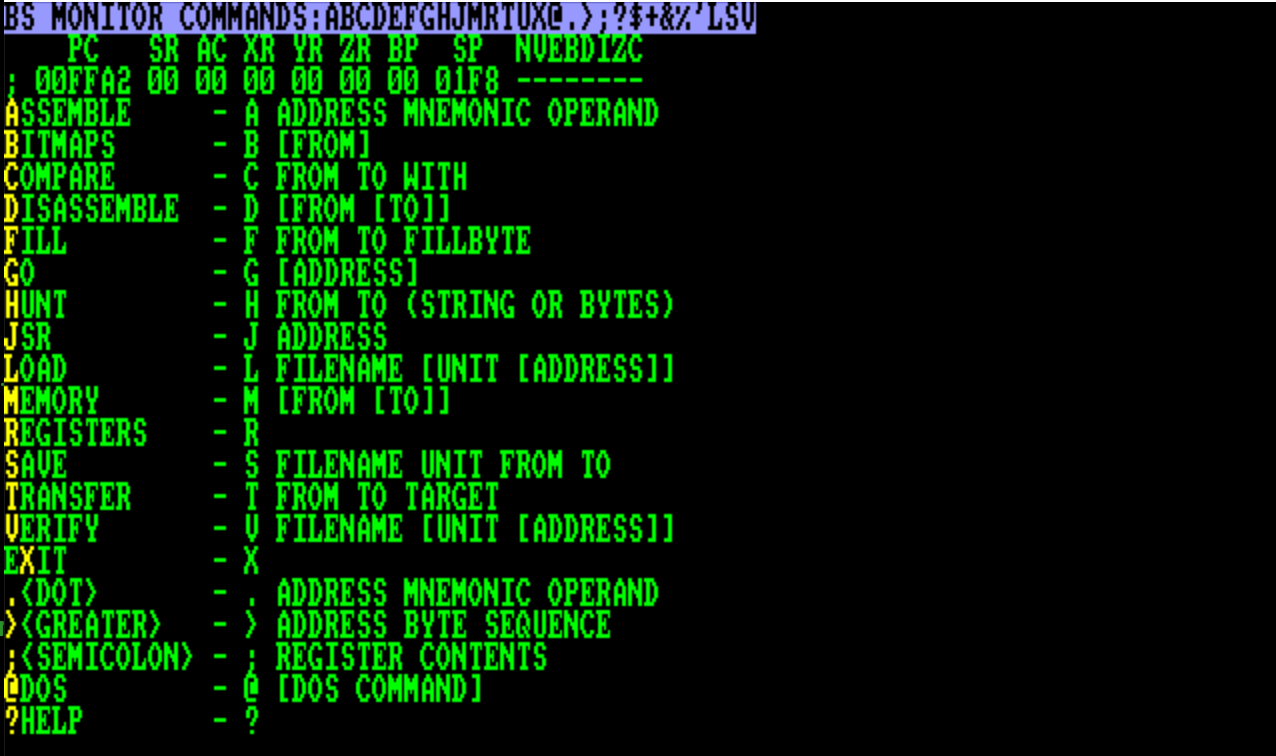
\includegraphics[width=0.8\linewidth]{images/monitor-h.png}
\end{center}

% *****
% MOUSE
% *****

\newpage
\subsection{MOUSE}
\index{MOUSE}
\index{BASIC 65 Commands!MOUSE}
\begin{description}[leftmargin=2cm,style=nextline]
\item [Token:] \$FE \$3E
\item [Format:] {\bf MOUSE ON [,port [,sprite [,pos]]]} \\
                {\bf MOUSE OFF}
\item [Usage:]  Enables the mouse driver
                and connects the mouse at the specified port
                with the mouse pointer sprite.

                {\bf port} = mouse port 1, 2 (default) or 3 (both).

                {\bf sprite} = sprite number for mouse pointer (default 0).

                {\bf pos} = initial mouse position (x,y).

                The {\bf MOUSE OFF} command disables the mouse
                driver and frees the associated sprite.

\item [Remarks:] The "hot spot" of the mouse pointer is the upper left
                pixel of the sprite.

\item [Example:] Using {\bf MOUSE}:
\begin{tcolorbox}[colback=black,coltext=white]
\verbatimfont{\codefont}
\begin{verbatim}
 REM LOAD DATA INTO SPRITE #0 BEFORE USING IT
 MOUSE ON, 1       :REM ENABLE  MOUSE WITH SPRITE #0
 MOUSE OFF         :REM DISABLE MOUSE
\end{verbatim}
\end{tcolorbox}
\end{description}

% ******
% MOVSPR
% ******

\newpage
\subsection{MOVSPR}
\index{MOVSPR}
\index{BASIC 65 Commands!MOVSPR}
\begin{description}[leftmargin=2cm,style=nextline]
\item [Token:] \$FE \$06
\item [Format:] {\bf MOVSPR number, position} \\
                {\bf MOVSPR number, start-position TO end-position, speed} \\
\item [Usage:]  Each position argument consists of two 16 bit values,
                which specify either an absolute coordinate, a relative coordinate,
                an angle or a speed. The value type is determined by a prefix:

                +value = relative coordinate: positive offset \\
                -value = relative coordinate: negative offset \\
                \#value = speed \\
                no prefix = absolute coordinate or angle

                So the position argument can be used to set the sprite
                to an absolute position on screen, to specify a displacement
                from the current position or describe a movement
                with angle and speed.

                The first format {\bf MOVSPR number, position} is used to
                set the sprite immediately to the position or, in case of
                an angle\#speed argument, describe its further movement.

                The second format
                {\bf MOVSPR number, start-position TO end-position, speed}
                puts the sprite into the start position and defines the
                destination position and the speed of movement.
                The sprite is put immediately to its start postion and will move
                on a straight line to the destination at the given speed.
                The movement is controlled by the BASIC interrupt handler and
                happens concurrently with the program execution.


                {\bf number} = sprite number (0-7)

                {\bf position} = x,y | xrel,y | x,yrel | xrel,yrel | angle\#speed

                {\bf x} = absolute screen coordinate [pixel].

                {\bf y} = absolute screen coordinate [pixel].

                {\bf xrel} = relative screen coordinate [pixel].

                {\bf yrel} = relative screen coordinate [pixel].

                {\bf angle} = direction for sprite movement [degrees].
                0 = up, 90 = right, 180 = down, 270 = left.

                {\bf speed} = speed of movement (0 -> 15).

\item [Remarks:] The "hot spot" is the upper left pixel of the sprite.

\item [Example:] Using {\bf MOVSPR}:
\begin{tcolorbox}[colback=black,coltext=white]
\verbatimfont{\codefont}
\begin{verbatim}
 10 SPRITE 1,1     :REM TURN SPRITE 1 ON
 20 MOVSPR 1,50,50 :REM SET SPRITE 1 to (50,50)
 30 MOVSPR 1,45#5  :REM MOVE SPRITE 1 WITH SPEED 5 TO UPPER RIGHT
 40 MOVSPR 1,320,10 TO -300,+150, 5 :REM MOVE SPRITE ON A LINE
\end{verbatim}
\end{tcolorbox}
\end{description}

% ***
% NEW
% ***

\newpage
\subsection{NEW}
\index{NEW}
\index{BASIC 65 Commands!NEW}
\begin{description}[leftmargin=2cm,style=nextline]
\item [Token:] \$A2
\item [Format:] {\bf NEW} \\
                {\bf NEW RESTORE}
\item [Usage:]  Resets all BASIC parameters
                to their default values.
                After {\bf NEW} the maximum RAM is available
                for program and data storage.

                Because {\bf NEW} resets parameters and pointers,
                but does not physically overwrite the address
                range of a BASIC program, that was in memory
                before {\bf NEW}, it is possible to recover the
                program. If there were no {\bf LOAD} operations
                or editing after the {\bf NEW} command, the program
                can be restored with the command \\
                {\bf NEW RESTORE}.
\item [Example:] Using {\bf NEW}:
\begin{tcolorbox}[colback=black,coltext=white]
\verbatimfont{\codefont}
\begin{verbatim}
 NEW         :REM RESET BASIC
 NEW RESTORE :REM TRY TO RECOVER NEW'ED PROGRAM
\end{verbatim}
\end{tcolorbox}
\end{description}

% ****
% NEXT
% ****

\newpage
\subsection{NEXT}
\index{NEXT}
\index{BASIC 65 Commands!NEXT}
\begin{description}[leftmargin=2cm,style=nextline]
\item [Token:] \$82
\item [Format:] {\bf FOR index=start TO end [STEP step] ... NEXT [index]}
\item [Usage:] Terminates the definition
               of a BASIC loop with an index variable.

               The {\bf index} variable may be incremented or decremented
               by a constant value {\bf step} on each iteration. The default
               is to increment the variable by 1.
               The index variable must be a real variable.

               The {\bf start} value is used to initialise the index.

               The {\bf end} value is used at the end of the loop
               and controls, whether the next iteration will be started
               or the loop exited.

               The {\bf step} value defines the change applied to
               to the index variable at the end of the loop.
               Positive step values increment it, while negative values
               decrement it. It defaults to 1.0 if not specified.

\item [Remarks:] The {\bf index} variable after {\bf NEXT} is
               optional. If it is missing, the variable
               for the current loop is assumed.
               Several consecutive {\bf NEXT} statements may be
               combined by specifying the indexes in a comma
               separated list. The statements
               {\bf NEXT I:NEXT J:NEXT K} and
               {\bf NEXT I,J,K} are equivalent.

\item [Example:] Using {\bf NEXT}
\begin{tcolorbox}[colback=black,coltext=white]
\verbatimfont{\codefont}
\begin{verbatim}
10 FOR D=0 TO 360 STEP 30
20 R = D * ~ / 180
30 PRINT D;R;SIN(R);COS(R);TAN(R)
40 NEXT D

10 DIM M(20,20)
20 FOR I=0 TO 20
30 FOR J=I TO 20
40 M(I,J) = I + 100 * J
50 NEXT J,I
\end{verbatim}
\end{tcolorbox}
\end{description}

% ***
% NOT
% ***

\newpage
\subsection{NOT}
\index{NOT}
\index{BASIC 65 Operators!NOT}
\begin{description}[leftmargin=2cm,style=nextline]
\item [Token:] \$A8
\item [Format:] {\bf NOT} operand
\item [Usage:]  Performs a bit-wise
                logical NOT operation on a 16 bit value.
                Integer operands are used as they are.
                Real operands are converted to a signed 16 bit integer.
                Logical operands are converted to 16 bit integer
                using \$FFFF, decimal -1 for TRUE
                and \$0000, decimal 0, for FALSE.

   \begin{verbatim}
      NOT 0  ->  1
      NOT 1  ->  0
   \end{verbatim}

\item [Remarks:] The result is of integer type.
                 If the result is used in a logical context,
                 the value of 0 is regarded as FALSE,
                 all other, nonzero values are regarded as TRUE.
\item [Example:] Using {\bf NOT}

\begin{tcolorbox}[colback=black,coltext=white]
\verbatimfont{\codefont}
\begin{verbatim}
  PRINT NOT 3
  -4
  PRINT NOT 64
  -65
\end{verbatim}
\end{tcolorbox}

In most cases the {\bf NOT} will be used in {\bf IF} statements.

\begin{tcolorbox}[colback=black,coltext=white]
\verbatimfont{\codefont}
\begin{verbatim}
   OK = C < 256 AND C >= 0
   IF (NOT OK) THEN PRINT "NOT A BYTE VALUE"
\end{verbatim}
\end{tcolorbox}
\end{description}

% ***
% OFF
% ***

\newpage
\subsection{OFF}
\index{OFF}
\index{BASIC 65 Commands!OFF}
\begin{description}[leftmargin=2cm,style=nextline]
\item [Token:] \$FE \$24
\item [Format:] keyword {\bf OFF}
\item [Usage:]  {\bf OFF} is a secondary keyword used in
                combination with primary keywords like
                {\bf COLOR, KEY, MOUSE}.

\item [Remarks:] The keyword {\bf OFF} cannot be used on its own.

\item [Example:] Using {\bf OFF}

\begin{tcolorbox}[colback=black,coltext=white]
\verbatimfont{\codefont}
\begin{verbatim}
  COLOR OFF :REM DISABLE SCREEN COLOUR
  KEY OFF   :REM DISABLE FUNCTION KEY STRINGS
  MOUSE OFF :REM DISABLE MOUSE DRIVER
\end{verbatim}
\end{tcolorbox}
\end{description}

% **
% ON
% **

\newpage
\subsection{ON}
\index{ON}
\index{BASIC 65 Commands!ON}
\begin{description}[leftmargin=2cm,style=nextline]
\item [Token:] \$91
\item [Format:] {\bf ON expression GOSUB line list} \\
                {\bf ON expression GOTO line list}  \\
                 keyword {\bf ON}
\item [Usage:]  The {\bf ON} keyword starts
                either a computed {\bf GOSUB} or {\bf GOTO} statement.
                Dependent on the value of the expression, the target
                for the {\bf GOSUB} or {\bf GOTO} is chosen from
                the table of line addresses at the end of the statement.

                As a secondary keyword, {\bf ON} is used in
                combination with primary keywords like
                {\bf COLOR, KEY, MOUSE}.

                {\bf expression} is a positive numeric value.
                Real values are cut to integer.

                {\bf line list} is a comma separated list of valid
                line numbers.

\item [Remarks:] Negative values for {\bf expression} will stop
                 the program with an error message.
                 The {\bf line list} specifies the targets for values
                 of 1,2,3,... \\
                 An expression value of zero or a value, that is greater
                 than the number of target lines will do nothing and
                 continue program execution with the next statement.

\newpage
\item [Example:] Using {\bf ON}
\begin{tcolorbox}[colback=black,coltext=white]
\verbatimfont{\codefont}
\begin{verbatim}
 10 COLOR ON :REM ENABLE SCREEN COLOUR
 20 KEY   ON :REM ENABLE FUNCTION KEY STRINGS
 30 MOUSE ON :REM ENABLE MOUSE DRIVER
 40 N = JOY(1):IF N AND 128 THEN PRINT "FIRE! ";
 60 REM                N   NE  E   SE  S   SW  W   NW
 70 ON N AND 15 GOSUB 100,200,300,400,500,600,700,800
 80 GOTO 40
100 PRINT "GO NORTH"    :RETURN
200 PRINT "GO NORTHEAST":RETURN
300 PRINT "GO EAST"     :RETURN
400 PRINT "GO SOUTHEAST":RETURN
500 PRINT "GO SOUTH"    :RETURN
600 PRINT "GO SOUTHWEST":RETURN
700 PRINT "GO WEST"     :RETURN
800 PRINT "GO NORTHWEST":RETURN
\end{verbatim}
\end{tcolorbox}
\end{description}

% ****
% OPEN
% ****

\newpage
\subsection{OPEN}
\index{OPEN}
\index{BASIC 65 Commands!OPEN}
\begin{description}[leftmargin=2cm,style=nextline]
\item [Token:] \$9F
\item [Format:]
  {\bf OPEN lfn, first address [,secondary address [,filename]]}
\item [Usage:]
   Opens an input/output channel for
   a device.

   {\bf lfn} = {\bf l}ogical {\bf f}ile {\bf n}umber \\
   1 <= lfn <= 127: line terminator is CR \\
   128 <= lfn <= 255: line terminator is CR LF

   {\bf first address} = device number.
   For IEC devices the unit number is the primary address.
   Following primary address values are possible:

{\setlength{\tabcolsep}{1mm}
\ttfamily
\begin{tabular}{|r|l|}
\hline
  unit  & device \\
\hline
  0 & Keyboard \\
  1 & System default \\
  2 & RS232 serial connection \\
  3 & Screen \\
  4-7 & IEC printer and plotter \\
  8-31 & IEC disk drives \\
\hline
\end{tabular}
}

   The {\bf secondary address} has some special values for
   IEC disk units, 0:load, 1:save, 15:command channel.
   The values 2 -> 14 may be used for disk files.

   {\bf filename} is either a quoted string, e.g. {\bf "data"} or
   a string expression. The syntax is different to the {\bf DOPEN\#}
   command. The {\bf filename} for {\bf OPEN} includes all
   file attributes, e.g.: "0:data,s,w".

\item [Remarks:]
   For IEC disk units the usage of {\bf DOPEN\#} is recommended.

   The usage of the "save-and-replace" character '@' at the
   beginning of the filename is not recommended, because many
   Commodore disk drives have a bug, that can cause data loss
   when using this feature.

\item [Example:] Using {\bf OPEN}

\begin{tcolorbox}[colback=black,coltext=white]
\verbatimfont{\codefont}
\begin{verbatim}
   OPEN 4,4   :REM OPEN PRINTER
   CMD 4      :REM REDIRECT STANDARD OUTPUT TO 4
   LIST       :REM PRINT LISTING ON PRINTER DEVICE 4
   OPEN 3,8,3,"0:USER FILE,U"
   OPEN 2,9,2,"0:DATA,S,W"
\end{verbatim}
\end{tcolorbox}
\end{description}

% **
% OR
% **

\newpage
\subsection{OR}
\index{OR}
\index{BASIC 65 Operators!OR}
\begin{description}[leftmargin=2cm,style=nextline]
\item [Token:] \$B0
\item [Format:] operand {\bf OR} operand
\item [Usage:]  Performs a bit-wise
                logical OR operation on two 16-bit values.
                Integer operands are used as they are.
                Real operands are converted to a signed 16-bit integer.
                Logical operands are converted to 16-bit integer
                using \$FFFF, decimal -1 for TRUE
                and \$0000, decimal 0, for FALSE.

   \begin{verbatim}
      0 OR 0  ->  0
      0 OR 1  ->  1
      1 OR 0  ->  1
      1 OR 1  ->  1
   \end{verbatim}

\item [Remarks:] The result is of integer type.
                 If the result is used in a logical context,
                 the value of 0 is regarded as FALSE,
                 all other, nonzero values are regarded as TRUE.
\item [Example:] Using {\bf OR}

\begin{tcolorbox}[colback=black,coltext=white]
\verbatimfont{\codefont}
\begin{verbatim}
  PRINT 1 OR 3
  3
  PRINT 128 OR 64
  192
\end{verbatim}
\end{tcolorbox}

In most cases the {\bf OR} will be used in {\bf IF} statements.

\begin{tcolorbox}[colback=black,coltext=white]
\verbatimfont{\codefont}
\begin{verbatim}
   IF (C < 0 OR C > 255) THEN PRINT "NOT A BYTE VALUE"
\end{verbatim}
\end{tcolorbox}
\end{description}

% *****
% PAINT
% *****

\newpage
\subsection{PAINT}
\index{PAINT}
\index{BASIC 65 Commands!PAINT}
\begin{description}[leftmargin=2cm,style=nextline]
\item [Token:] \$DF
\item [Format:] {\bf PAINT x, y, mode [,colour]}
\item [Usage:]  Performs a flood fill
                of an enclosed graphics area.

                {\bf x, y} is a coordinate pair, which must
                lie inside the area to be filled.

                {\bf mode} specifies the fill mode. \\
                0: use the {\bf colour} to fill the area. \\
                1: use the colour of pixel (x,y) to fill the area.

\item [Example:] Using {\bf PAINT}

\begin{tcolorbox}[colback=black,coltext=white]
\verbatimfont{\codefont}
\begin{verbatim}
 10 GRAPHIC CLR          :REM INITIALISE
 20 SCREEN DEF 1,0,0,2   :REM 320 X 200
 30 SCREEN OPEN 1        :REM OPEN
 40 SCREEN SET 1,1       :REM MAKE SCREEN ACTIVE
 50 LINE 160,0,240,100   :REM 1ST. LINE
 60 LINE 240,100,80,100  :REM 2ND. LINE
 70 LINE 80,100,160,0    :REM 3RD. LINE
 80 PAINT 160,10,0,1     :REM FILL TRIANGLE WITH COLOUR 1
 90 GETKEY K$            :REM WAIT FOR KEY
100 SCREEN CLOSE 1       :REM END GRAPHICS
\end{verbatim}
\end{tcolorbox}
\end{description}

% *******
% PALETTE
% *******

\newpage
\subsection{PALETTE}
\index{PALETTE}
\index{BASIC 65 Commands!PALETTE}
\begin{description}[leftmargin=2cm,style=nextline]
\item [Token:] \$FE \$34
\item [Format:] {\bf PALETTE [screen|COLOR], colour, red, green, blue} \\
                {\bf PALETTE RESTORE}
\item [Usage:]  The {\bf PALETTE} command can be used to change an
                entry of the system colour palette or the palette
                of a screen. \\
                {\bf PALETTE RESTORE} resets the system palette to
                the default values.

                {\bf screen} = screen number 0 -> 3.

                {\bf COLOR} = keyword for changing system palette.

                {\bf colour} = index to palette 0 -> 255.

                {\bf red} = red intensity 0 -> 15.

                {\bf green} = green intensity 0 -> 15.

                {\bf blue} = blue intensity 0 -> 15.

\item [Example:] Using {\bf PALETTE}

\begin{tcolorbox}[colback=black,coltext=white]
\verbatimfont{\codefont}
\begin{verbatim}
 10 GRAPHIC CLR             :REM INITIALISE
 20 SCREEN DEF 1,0,0,2      :REM 320 X 200
 30 SCREEN OPEN 1           :REM OPEN
 40 SCREEN SET 1,1          :REM MAKE SCREEN ACTIVE
 50 PALETTE 1,0,  0, 0, 0   :REM 0 = BLACK
 60 PALETTE 1,1, 15, 0, 0   :REM 1 = RED
 70 PALETTE 1,2,  0, 0,15   :REM 2 = BLUE
 80 PALETTE 1,3,  0,15, 0   :REM 3 = GREEN
 90 LINE 160,0,240,100      :REM 1ST. LINE
100 LINE 240,100,80,100     :REM 2ND. LINE
110 LINE 80,100,160,0       :REM 3RD. LINE
120 PAINT 160,10,0,2        :REM FILL TRIANGLE WITH BLUE (2)
130 GETKEY K$               :REM WAIT FOR KEY
140 SCREEN CLOSE 1          :REM END GRAPHICS
\end{verbatim}
\end{tcolorbox}
\end{description}

% ****
% PEEK
% ****

\newpage
\subsection{PEEK}
\index{PEEK}
\index{BASIC 65 Functions!PEEK}
\begin{description}[leftmargin=2cm,style=nextline]
\item [Token:] \$C2
\item [Format:] {\bf PEEK(address)}
\item [Usage:]  Returns an unsigned 8 bit value (byte)
                read from address.

                If the address is in the range (\$0000 to \$FFFF) the
                memory bank (set by {\bf BANK}) is used.

                Addresses >= \$10000 are assumed to be flat memory
                addresses and used as such, ignoring the bank setting.

\item [Remarks:] Banks 0 -> 127 give access to RAM or ROM banks.
                 Banks > 127 are used to access I/O and SYSTEM
                 like VIC, SID, FDC, etc.
\item [Example:] Using {\bf PEEK}

\begin{tcolorbox}[colback=black,coltext=white]
\verbatimfont{\codefont}
\begin{verbatim}
 10 BANK 128                :REM SELECT SYSTEM BANK
 20 L = PEEK($02F8)         :REM USR JUMP TARGET LOW
 30 H = PEEK($02F9)         :REM USR JUMP TARGET HIGH
 40 T = L + 256 * H         :REM 16 BIT JUMP ADDRESS
 50 PRINT "USR FUNCTION CALLS ADDRESS";T
\end{verbatim}
\end{tcolorbox}
\end{description}

% *****
% PEEKW
% *****

\newpage
\subsection{PEEKW}
\index{PEEKW}
\index{BASIC 65 Functions!PEEKW}
\begin{description}[leftmargin=2cm,style=nextline]
\item [Token:] \$C2 'W'
\item [Format:] {\bf PEEKW(address)}
\item [Usage:]  Returns an unsigned 16 bit value (word)
                read from address (low byte) and address+1 (high byte).

                If the address is in the range (\$0000 to \$FFFF) the
                memory bank (set by {\bf BANK}) is used.

                Addresses >= \$10000 are assumed to be flat memory
                addresses and used as such, ignoring the bank setting.


\item [Remarks:] Banks 0 -> 127 give access to RAM or ROM banks.
                 Banks > 127 are used to access I/O and SYSTEM
                 like VIC, SID, FDC, etc.
\item [Example:] Using {\bf PEEKW}

\begin{tcolorbox}[colback=black,coltext=white]
\verbatimfont{\codefont}
\begin{verbatim}
 20 UA = PEEKW($02F8)   :REM USR JUMP TARGET
 50 PRINT "USR FUNCTION CALL ADDRESS";UA
\end{verbatim}
\end{tcolorbox}
\end{description}

% ***
% PEN
% ***

\newpage
\subsection{PEN}
\index{PEN}
\index{BASIC 65 Commands!PEN}
\begin{description}[leftmargin=2cm,style=nextline]
\item [Token:] \$FE \$33
\item [Format:] {\bf PEN pen colour}
\item [Usage:]  Sets the colour for the graphic pen.

                {\bf pen} = pen number ( 0 -> 2 )

                {\bf colour} = palette index.

\item [Remarks:] {\bf PEN} defined colours are used by all
                 following drawing commands.

\item [Example:] Using {\bf PEN}

\begin{tcolorbox}[colback=black,coltext=white]
\verbatimfont{\codefont}
\begin{verbatim}
 10 GRAPHIC CLR             :REM INITIALISE
 20 SCREEN DEF 1,0,0,2      :REM 320 X 200
 30 SCREEN OPEN 1           :REM OPEN
 40 SCREEN SET 1,1          :REM MAKE SCREEN ACTIVE
 50 PALETTE 1,0,  0, 0, 0   :REM 0 = BLACK
 60 PALETTE 1,1, 15, 0, 0   :REM 1 = RED
 70 PALETTE 1,2,  0, 0,15   :REM 2 = BLUE
 80 PALETTE 1,3,  0,15, 0   :REM 3 = GREEN
 90 PEN 0,1                 :REM PEN 0 = RED
100 LINE 160,0,240,100      :REM DRAW RED LINE
110 PEN 0,2                 :REM PEN 0 = BLUE
120 LINE 240,100,80,100     :REM DRAW BLUE LINE
130 PEN 0,3                 :REM PEN 0 = GREEN
140 LINE 80,100,160,0       :REM DRAW GREEN LINE
150 GETKEY K$               :REM WAIT FOR KEY
160 SCREEN CLOSE 1          :REM END GRAPHICS
\end{verbatim}
\end{tcolorbox}
\end{description}



% *****
% PIXEL
% *****

\newpage
\subsection{PIXEL}
\index{PIXEL}
\index{BASIC 65 Functions!PIXEL}
\begin{description}[leftmargin=2cm,style=nextline]
\item [Token:] \$CE \$0C
\item [Format:] {\bf PIXEL(x,y)}
\item [Usage:]  Returns colour at given position.

               {\bf x} = absolute screen coordinate [pixel].

               {\bf y} = absolute screen coordinate [pixel].
\end{description}


% ****
% PLAY
% ****

\newpage
\subsection{PLAY}
\index{PLAY}
\index{BASIC 65 Commands!PLAY}
\begin{description}[leftmargin=2cm,style=nextline]
\item [Token:] \$FE \$04
\item [Format:] {\bf PLAY string}
\item [Usage:] Starts playing a tune with notes and directives
               embedded in the argument string.

               A musical note is a letter (A,B,C,D,E,F,G)
               which may be preceded by an optional modifier.

               Possible modifiers are:

{\setlength{\tabcolsep}{1mm}
\ttfamily
\begin{tabular}{*{1}{|R{9mm}}|l|}
\hline
 char  & effect \\
\hline
 \# & sharp \\
 \$ & flat \\
  . & dotted \\
  H & half note \\
  I & eighth note \\
  M & wait for end \\
  Q & quarter note \\
  R & pause (rest) \\
  S & sixteenth note \\
  W & whole note \\
\hline
\end{tabular}
}

Embedded directives consist of a letter followed by a digit:

{\setlength{\tabcolsep}{1mm}
\ttfamily
\begin{tabular}{*{1}{|R{9mm}}|l|l|}
\hline
 char  & directive & argument range \\
\hline
  O & octave        & 0 - 6 \\
  T & tune envelope & 0 - 9 \\
  U & volume        & 0 - 9 \\
  V & voice         & 1 - 3 \\
  X & filter        & 0 - 1 \\
\hline
\end{tabular}
}

\newpage

The envelope slots may be changed using the {\bf ENVELOPE}
statement. The default setting for the envelopes are:

{\setlength{\tabcolsep}{1mm}
\ttfamily
\begin{tabular}{*{6}{|R{5mm}}|R{9mm}|l|}
\hline
 n  & A & D & S & R & WF & PW & Instrument \\
\hline
  0 & 0 &  9 &  0 &  0 &  2 &  1536  &     piano \\
  1 & 12&  0 & 12 &  0 &  1 &        &     accordion \\
  2 & 0 &  0 & 15 &  0 &  0 &        &     calliope \\
  3 & 0 &  5 &  5 &  0 &  3 &        &     drum \\
  4 & 9 &  4 &  4 &  0 &  0 &        &     flute \\
  5 & 0 &  9 &  2 &  1 &  1 &        &     guitar \\
  6 & 0 &  9 &  0 &  0 &  2 &  512   &     harpsichord \\
  7 & 0 &  9 &  9 &  0 &  2 &  2048  &     organ \\
  8 & 8 &  9 &  4 &  1 &  2 &  512   &     trumpet \\
  9 & 0 &  9 &  0 &  0 &  0 &        &     xylophone \\
\hline
\end{tabular}
}

\item [Remarks:] The {\bf PLAY} statement sets up an interrupt
                 driven routine that starts parsing the string
                 and playing the tune. The execution continues
                 with the next statement with no need waiting for
                 the tune to be finished. However this can be
                 forced, using the 'M' modifier.


\item [Example:] Using {\bf PLAY}
\begin{tcolorbox}[colback=black,coltext=white]
\verbatimfont{\codefont}
\begin{verbatim}
10 ENVELOPE 9,10,5,10,5,2,4000
20 PLAY "T9"
30 VOL 8
40 TEMPO 100
50 PLAY "C D E F G A B"
60 PLAY "U5 V1 C D E F G A B"
\end{verbatim}
\end{tcolorbox}
\end{description}

% *******
% POINTER
% *******

\newpage
\subsection{POINTER}
\index{POINTER}
\index{BASIC 65 Functions!POINTER}
\begin{description}[leftmargin=2cm,style=nextline]
\item [Token:] \$CE \$0A
\item [Format:] {\bf POINTER(variable)}
\item [Usage:]  Returns the current address of a variable
                or an array element.
                For string variables, it is the address of
                the string descriptor, not the string itself.
                The string descriptor consists of the three bytes
                (length,string address low, string address high).

                Address values $>=$ \$F700 are assigned to bank 0.
                All other addresses are assigned to bank 1.

\item [Remarks:] The address values of arrays and their elements
                 are constant during a program execution. \\
                 The addresses of strings (not their descriptors)
                 however may change at any time due to
                 "garbage collection" in memory management.


\item [Example:] Using {\bf POINTER}

\begin{tcolorbox}[colback=black,coltext=white]
\verbatimfont{\codefont}
\begin{verbatim}
10 H$="HELLO"
20 P=POINTER(H$):PRINT "DESCRIPTOR AT: $";HEX$(P)
30 IF P>= DEC("F700") THENBANK 0:ELSEBANK 1
40 L=PEEK(P):SP=PEEK(P+1)+256*PEEK(P+2)
50 PRINT"STRING ADDRESS:$";HEX$(SP)
60 PRINT "LENGTH=";L
70 BANK 1:REM STRING BANK
80 FOR I=1TOL:PRINT PEEK(SP+I-1);:NEXT:PRINT
90 FOR I=1TOL:PRINT CHR$(PEEK(SP+I-1));:NEXT:PRINT

RUN
DESCRIPTOR AT: $F702
STRING ADDRESS:$F6F9
LENGTH= 5
 72  69  76  76  79
HELLO
\end{verbatim}
\end{tcolorbox}
\end{description}

% ****
% POKE
% ****

\newpage
\subsection{POKE}
\index{POKE}
\index{BASIC 65 Functions!POKE}
\begin{description}[leftmargin=2cm,style=nextline]
\item [Token:] \$97
\item [Format:] {\bf POKE address, byte [,byte ...] }
\item [Usage:]  Puts on or more bytes into memory
                or memory mapped I/O, starting at
                {\bf address}.

                If the address is in the range (\$0000 to \$FFFF) the
                memory bank (set by {\bf BANK}) is used.

                Addresses >= \$10000 are assumed to be flat memory
                addresses and used as such, ignoring the bank setting.

                {\bf byte} = a value 0 -> 255.

\item [Remarks:] The address is increased by one for each data byte,
                 so a memory range may be filled with a single command.

                 Banks > 127 are used to access I/O and SYSTEM
                 like VIC, SID, FDC, etc.
\item [Example:] Using {\bf POKE}

\begin{tcolorbox}[colback=black,coltext=white]
\verbatimfont{\codefont}
\begin{verbatim}
 10 BANK 128                :REM SELECT SYSTEM BANK
 20 POKE $02F8"),0,24       :REM SET USR VECTOR TO $1800
\end{verbatim}
\end{tcolorbox}
\end{description}

% *****
% POKEW
% *****

\newpage
\subsection{POKEW}
\index{POKEW}
\index{BASIC 65 Functions!POKEW}
\begin{description}[leftmargin=2cm,style=nextline]
\item [Token:] \$97 'W'
\item [Format:] {\bf POKEW address, word [,word ...] }
\item [Usage:]  Puts on or more words into memory
                or memory mapped I/O, starting at
                {\bf address}.

                If the address is in the range (\$0000 to \$FFFF) the
                memory bank (set by {\bf BANK}) is used.

                Addresses >= \$10000 are assumed to be flat memory
                addresses and used as such, ignoring the bank setting.

                {\bf word} = a value 0 -> 65535

                The first word is stored at address (low byte)
                and address+1 (high byte). The second one at
                address+2 (low byte) and address+3 (high byte), etc.

\item [Remarks:] The address is increased by two for each data word,
                 so a memory range may be filled with a single PEEKW command.

                 Banks > 127 are used to access I/O and SYSTEM
                 like VIC, SID, FDC, etc.
\item [Example:] Using {\bf POKEW}

\begin{tcolorbox}[colback=black,coltext=white]
\verbatimfont{\codefont}
\begin{verbatim}
 10 BANK 128                :REM SELECT SYSTEM BANK
 20 POKEW $02F8,$1800       :REM SET USR VECTOR TO $1800
\end{verbatim}
\end{tcolorbox}
\end{description}

% *******
% POLYGON
% *******

\newpage
\subsection{POLYGON}
\index{POLYGON}
\index{BASIC 65 Commands!POLYGON}

\begin{description}[leftmargin=2cm,style=nextline]
\item [Token:] \$FE \$2F
\item [Format:] {\bf POLYGON x, y, xrad, yrad, solid, angle,
                sides, n}

\item [Usage:] Draws a regular {\bf n} sided polygon.
               The polygon is drawn using the current drawing context
               set with SCREEN, PALETTE and PEN.

               {\bf x,y} = centre coordinates.

               {\bf xrad,yrad} = radius in x- and y-direction.

               {\bf solid} = fill (1) or outline (0).

               {\bf angle} = start angle.

               {\bf sides} = sides to draw $(<= n)$.

               {\bf n} = number of sides or edges.

\item [Remarks:] A regular polygon is both isogonal and isotoxal,
                 meaning all sides and angles are alike.

\item [Example:] Using {\bf POLYGON}
\begin{tcolorbox}[colback=black,coltext=white]
\verbatimfont{\codefont}
\begin{verbatim}
  POLYGON 320,100,50,50,0,0,6,6
\end{verbatim}
\end{tcolorbox}
\begin{tikzpicture}[thick]
\draw (8cm,4cm) -- (6cm,6mm) -- (2cm,6mm) -- (0cm,4cm) -- (2cm,74mm) -- (6cm,74mm) -- (8cm,4cm);
\end{tikzpicture}
\end{description}

% ***
% POS
% ***

\newpage
\subsection{POS}
\index{POS}
\index{BASIC 65 Functions!POS}
\begin{description}[leftmargin=2cm,style=nextline]
\item [Token:] \$B9
\item [Format:] {\bf POS(dummy)}
\item [Usage:]  Returns the cursor column relative to the
                currently used window.

                {\bf dummy} = a numeric value, which is ignored.

\item [Remarks:] {\bf POS} gives the column position for the screen
                 cursor. It will not work for redirected output.

\item [Example:] Using {\bf POS}

\begin{tcolorbox}[colback=black,coltext=white]
\verbatimfont{\codefont}
\begin{verbatim}
 10 IF POS(0) > 72 THEN PRINT :REM INSERT RETURN
\end{verbatim}
\end{tcolorbox}
\end{description}

% ***
% POT
% ***

\newpage
\subsection{POT}
\index{POT}
\index{BASIC 65 Functions!POT}
\begin{description}[leftmargin=2cm,style=nextline]
\item [Token:] \$CE \$02
\item [Format:] {\bf POT(paddle)}
\item [Usage:]  Returns the position of a paddle.

                {\bf paddle} = paddle number 1 -> 4.

                The low byte of the return value is the
                paddle value
                with 0 at the clockwise limit and 255 at the
                counterclockwise limit.

                A value > 255 indicates the simultaneous press
                of the fire button.

\item [Remarks:] Analogue paddles are noisy and inexact.
                 The range may be less than 0 - 255 and there
                 is some jitter in the data.


\item [Example:] Using {\bf POT}

\begin{tcolorbox}[colback=black,coltext=white]
\verbatimfont{\codefont}
\begin{verbatim}
 10 X = POT(1)       : REM READ PADDLE #1
 20 B = X > 255      : REM TRUE (-1) IF FIRE BUTTON IS PRESSED
 30 V = X AND 255    : PADDLE #1 VALUE
\end{verbatim}
\end{tcolorbox}
\end{description}

% *****
% PRINT
% *****

\newpage
\subsection{PRINT}
\index{PRINT}
\index{BASIC 65 Commands!PRINT}
\begin{description}[leftmargin=2cm,style=nextline]
\item [Token:] \$99
\item [Format:] {\bf PRINT arguments}
\item [Usage:]  Evaluates the argument list and prints the values
                formatted to the current screen window.
                Standard formatting is used dependent on the
                argument type. For user controlled formatting
                see {\bf PRINT USING}.
                Following argument types are processed:

                {\bf numeric} : The printout starts with a space
                for positive and zero values or a minus sign for
                negative values. Integer values are printed with
                the necessary number of digits. Real values are
                printed either in fixed point format with typically
                9 digits or in scientific format, if the value is
                outside the range of 0.01 -> 999999999.

                {\bf string} : The string may consist of printable
                characters and control codes. Printable characters
                are printed to the cursor position, while control
                codes are executed.

                {\bf ,} : A comma acts like a tabulator.

                {\bf ;} : A semicolon acts as a separator between
                arguments of the list. Other than the comma character
                it does not put in any additional characters.
                A semicolon at the end of the argument list suppresses
                the automatic return character.

\item [Remarks:] The {\bf SPC} and {\bf TAB} functions
                 may be used in the argument list
                 for positioning.
                 The {\bf CMD} command can be used for redirection.

\item [Example:] Using {\bf PRINT}

\begin{tcolorbox}[colback=black,coltext=white]
\verbatimfont{\codefont}
\begin{verbatim}
 10 FOR I=1 TO 10    : REM START LOOP
 20 PRINT I,I*I,SQR(I)
 30 NEXT
\end{verbatim}
\end{tcolorbox}
\end{description}

% ******
% PRINT#
% ******

\newpage
\subsection{PRINT\#}
\index{PRINT\#}
\index{BASIC 65 Commands!PRINT\#}
\begin{description}[leftmargin=2cm,style=nextline]
\item [Token:] \$98
\item [Format:] {\bf PRINT\# channel, arguments}
\item [Usage:]  Evaluates the argument list and prints the values
                formatted to the device assigned to {\bf channel}.
                Standard formatting is used dependent on the
                argument type. For user controlled formatting
                see {\bf PRINT\# USING}.
                Following argument types are processed:

                {\bf channel} : must be opened for output by
                an {\bf OPEN} or {\bf DOPEN} statement.

                {\bf numeric} : The printout starts with a space
                for positive and zero values or a minus sign for
                negative values. Integer values are printed with
                the necessary number of digits. Real values are
                printed either in fixed point format with typically
                9 digits or in scientific format, if the value is
                outside the range of 0.01 -> 999999999.

                {\bf string} : The string may consist of printable
                characters and control codes. Printable characters
                are printed to the cursor position, while control
                codes are executed.

                {\bf ,} : A comma acts like a tabulator.

                {\bf ;} : A semicolon acts as a separator between
                arguments of the list. Other than the comma character
                it does not put in any additional characters.
                A semicolon at the end of the argument list suppresses
                the automatic return character.

\item [Remarks:] The {\bf SPC} and {\bf TAB} functions
                 are not suitable for devices other than the screen.

\item [Example:] Using {\bf PRINT\#}

\begin{tcolorbox}[colback=black,coltext=white]
\verbatimfont{\codefont}
\begin{verbatim}
 10 DOPEN#2,"TABLE",W,U9
 20 FOR I=1 TO 10    : REM START LOOP
 30 PRINT#2,I,I*I,SQR(I)
 40 NEXT
 50 DCLOSE#2
\end{verbatim}
\end{tcolorbox}
\end{description}

% ***********
% PRINT USING
% ***********

\newpage
\subsection{PRINT USING}
\index{PRINT USING}
\index{BASIC 65 Commands!PRINT USING}
\begin{description}[leftmargin=2cm,style=nextline]
\item [Token:] \$98 \$FB or \$99 \$FB
\item [Format:] {\bf PRINT [\# channel,] USING format;argument}
\item [Usage:]  Parses the format string and evaluates the argument.
                The argument can be either a string or a numeric value.
                The formatting of the resulting output is directed
                by the format string.

                {\bf channel} : must be opened for output by
                an {\bf OPEN} or {\bf DOPEN} statement.
                If no channel is specified, the output goes to the screen.

                {\bf format} : A string variable or a string constant
                which defines the rules for formatting.

                {\bf numeric argument} :
                The numeric formatting can be done in either
                CBM style providing a pattern like
                {\ttfamily "\#\#\#.\#\#"}
                or in C style using width.precision specifier like
                {\ttfamily \%3D \%7.2F \%4X } for example.

                If the argument does not fit into the format
                e.g. trying to print a 4 digit varaible into "\#\#\#"
                a series of asterisks fills the format character.

                {\bf string argument} : The string may consist of printable
                characters and control codes. Printable characters
                are printed to the cursor position, while control
                codes are executed.
                The number of '\#' characters sets the width of the output.
                If the first character of the format string
                is a '=' sign, the argument string is centered within
                the width.
                If the first character of the format string
                is a '>' sign, the argument string is right justified within
                the width.

\item [Remarks:] The format string is applied for one argument only.
                 But it is possible to append more than one
                 USING format;argument sequence.


\newpage
\item [Example:] Using {\bf PRINT\# USING}

\begin{tcolorbox}[colback=black,coltext=white]
\verbatimfont{\codefont}
\begin{verbatim}
PRINT USING "##.##";~, USING " [%6.4F] ";SQR(2)
 3.14 [1.4142]

PRINT USING " < # # # > ";12*31
 < 3 7 2 >

PRINT USING "###"; "ABCDE"
ABC

PRINT USING ">###"; "ABCDE"
CDE

PRINT USING "ADDRESS:$%4X";65000
ADDRESS:$FDE8

A$="###,###,###.#":PRINT USING A$;1E8/3
 33,333,333.3
\end{verbatim}
\end{tcolorbox}
\end{description}

% *****
% PUDEF
% *****

%\newpage
%\subsection{PUDEF}
%\index{PUDEF}
%\index{BASIC 65 Commands!PUDEF}
%\begin{description}[leftmargin=2cm,style=nextline]
%\item [Token:] \$DD
%\item [Format:] {\bf PUDEF string}
%\item [Usage:]  Redefines up to four special characters, that are
%                used in the {\bf PRINT USING} routine.
%
%                {\bf string} = definition string (max. 4 characters).
%
%{\ttfamily
%                1st.: fill character \\
%                2nd.: comma separator \\
%                3rd.: decimal point \\
%                4th.: currency symbol
%
%                The system default is " ,.\$"
%}
%
%                The new definition string overrides the system
%                default and is often used for localisation.
%                A string " .," would change the punctuation to
%                German style.
%
%                It is not necessary to redefine all four characters.
%                Any length between 1 and 4 is allowed.
%
%\item [Remarks:] {\bf PUDEF} changes the output of {\bf PRINT USING}
%                 only. {\bf PRINT} and {\bf PRINT\#} are not affected.
%                 The control characters of the format string
%                 cannot be changed.
%
%\item [Example:] Using {\bf PUDEF}
%
%\begin{tcolorbox}[colback=black,coltext=white]
%\verbatimfont{\codefont}
%\begin{verbatim}
% 10 X = 123456.78
% 20 PUDEF " .,"
% 30 PRINT USING "###,###.#"; X : REM 123.456,8
%\end{verbatim}
%\end{tcolorbox}
%\end{description}

% ******
% RCOLOR
% ******

\newpage
\subsection{RCOLOR}
\index{RCOLOR}
\index{BASIC 65 Functions!RCOLOR}
\begin{description}[leftmargin=2cm,style=nextline]
\item [Token:] \$CD
\item [Format:] {\bf RCOLOR(colour source)}
\item [Usage:]  Returns the current colour index for the
                selected colour source.

                Colour sources are:

{\ttfamily
                0: background colour (VIC \$D021) \\
                1: text colour (\$F1) \\
                2: highlight colour (\$2D8) \\
                3: border colour (VIC \$D020)
}
\item [Example:] Using {\bf RCOLOR}

\begin{tcolorbox}[colback=black,coltext=white]
\verbatimfont{\codefont}
\begin{verbatim}
 10 C = RCOLOR(3)  : REM C = colour index of border colour
\end{verbatim}
\end{tcolorbox}
\end{description}

% ****
% READ
% ****

\newpage
\subsection{READ}
\index{READ}
\index{BASIC 65 Commands!READ}
\begin{description}[leftmargin=2cm,style=nextline]
\item [Token:] \$87
\item [Format:] {\bf READ variable list}
\item [Usage:]  Reads values from program source into variables.

                {\bf variable list} = any legal variables.

               All type of constants (integer, real,
               strings) can be read, but no expressions.
               Items are separated by commas.
               Strings containing commas, colons or spaces must be put
               in quotes. \\
               A {\bf RUN} command initialises the data pointer
               to the first item of the first {\bf DATA} statement
               and advances it for every read item. It is in the
               responsibility of the programmer, that the type of
               the constant and the variable in the {\bf READ}
               statement match. Empty items with no constant
               between commas are allowed and will be interpreted as
               zero for numeric variables and an empty string for
               string variables. \\
               The {\bf RESTORE} command may be used to set the
               data pointer to a specific line for subsequent
               readings.

\item [Remarks:] It is good programming style to put large amount of
               {\bf DATA} statements at the end of the program.
               Otherwise {\bf GOTO} and {\bf GOSUB} statements, with
               target lines lower than the current one,
               start their search for linenumber at the beginning of
               the program and have to skip through {\bf DATA} lines
               wasting time.
\item [Example:] Using {\bf READ}
\begin{tcolorbox}[colback=black,coltext=white]
\verbatimfont{\codefont}
\begin{verbatim}
10 READ NA$, VE
20 READ N%:FOR I=2 TO N%:READ GL(I):NEXT I
30 PRINT "PROGRAM:";NA$;"   VERSION:";VE
40 PRINT "N-POINT GAUSS-LEGENDRE FACTORS E1":
50 FOR I=2 TO N%:PRINT I;GL(I):NEXT I
30 STOP
80 DATA "MEGA65",1.1
90 DATA 5,0.5120,0.3573,0.2760,0.2252
\end{verbatim}
\end{tcolorbox}
\end{description}

% ******
% RECORD
% ******

\newpage
\subsection{RECORD}
\index{RECORD}
\index{BASIC 65 Commands!RECORD}
\begin{description}[leftmargin=2cm,style=nextline]
\item [Token:] \$FE \$12
\item [Format:] {\bf RECORD\#lfn, record, [,byte]}
\item [Usage:]  Positions the read/write pointer of a relative file.

                {\bf lfn} = {\bf l}ogical {\bf f}ile {\bf n}umber

                {\bf record} = target record ( 1 -> 65535 ).

                {\bf byte} = byte position in record.

                This command can be used only for files of
                type {\bf REL}, which are relative files capable
                of direct access.

               The {\bf RECORD} command positions the file pointer
               to the specified record number. If this record number
               does not exist and the disk capacity is high enough,
               the file is expanded to this record count by adding
               empty records. This is not an error, but the disk
               status will give the message {\bf RECORD NOT PRESENT}.

               Any INPUT\# or PRINT\# command will then proceed
               on the selected record position.

\item [Remarks:] The original Commodore disk drives all had a bug
               in their DOS, which could destroy data by using
               relative files. A recommended workaround was to
               issue each {\bf RECORD} command twice, before
               and after the I/O operation.

\item [Example:] Using {\bf RECORD}
\begin{tcolorbox}[colback=black,coltext=white]
\verbatimfont{\codefont}
\begin{verbatim}
10 REM *** READ FIRST 10 INDEXED RECORDS FROM DATA BASE
15 N = 1000: DIM IX(N)
20 DOPEN#3,"DATA INDEX"
25 FOR I=1 TO N:INPUT#3,IX(I):NEXT
30 DCLOSE#3
35 DOPEN#2,"DATA BASE",L240
40 FOR J=1 TO 10
45 RECORD#2,IX(J)
50 INPUT#2,A$
55 PRINT A$
60 NEXT J
65 DCLOSE#2
\end{verbatim}
\end{tcolorbox}
\end{description}

% ***
% REM
% ***

\newpage
\subsection{REM}
\index{REM}
\index{BASIC 65 Commands!REM}
\begin{description}[leftmargin=2cm,style=nextline]
\item [Token:] \$8F
\item [Format:] {\bf REM}
\item [Usage:]  Marks the rest of the line as comment.

                All characters after {\bf REM} are never executed
                but skipped.

\item [Example:] Using {\bf REM}

\begin{tcolorbox}[colback=black,coltext=white]
\verbatimfont{\codefont}
\begin{verbatim}
 10 REM *** PROGRAM TITLE ***
 20 N=1000 :REM NUMBER OF ITEMS
 30 DIM NA$(N)
\end{verbatim}
\end{tcolorbox}
\end{description}

% ******
% RENAME
% ******

\newpage
\subsection{RENAME}
\index{RENAME}
\index{BASIC 65 Commands!RENAME}
\begin{description}[leftmargin=2cm,style=nextline]
\item [Token:] \$F5
\item [Format:] {\bf RENAME old TO new [,D drive] [,U unit] }
\item [Usage:] Renames a disk file.

   {\bf old} is either a quoted string, e.g. {\bf "data"} or
   a string expression in parentheses, e.g. {\bf (FI\$)}.

   {\bf new} is either a quoted string, e.g. {\bf "backup"} or
   a string expression in parentheses, e.g. {\bf (FS\$)}

   \drivedefinition

   \unitdefinition

\item [Remarks:]
   The {\bf RENAME} command is executed in the DOS of the disk drive.
   It can rename all regular file types (PRG, SEQ, USR, REL).
   The old file must exist, the new file must not exist.
   Only single files can be renamed, wild characters like
   '*' and '?' are not allowed. The file type cannot be changed.

\item [Example:] Using {\bf RENAME}
\begin{tcolorbox}[colback=black,coltext=white]
\verbatimfont{\codefont}
\begin{verbatim}
  RENAME "CODES" TO "BACKUP" :REM RENAME SINGLE FILE
\end{verbatim}
\end{tcolorbox}
\end{description}

% ********
% RENUMBER
% ********

\newpage
\subsection{RENUMBER}
\index{RENUMBER}
\index{BASIC 65 Commands!RENUMBER}
\begin{description}[leftmargin=2cm,style=nextline]
\item [Token:] \$F8
\item [Format:] {\bf RENUMBER [new [,inc [range]]]}
\item [Usage:] Used to renumber all or
               a range of lines of a BASIC program.

               {\bf new } is the new starting line of the
               line range to renumber.
               The default value is 10.

               {\bf inc } is the increment to be used.
               The default value is 10.

               {\bf range } is the line range to renumber.
               The default values are from first to last line.

               The {\bf RENUMBER} changes all line numbers in
               the chosen range and also changes all references
               from statements like {\bf GOTO, GOSUB, TRAP,
               RESTORE, RUN} etc.

               {\bf RENUMBER} can be executed in direct mode only.
               If it detects a problem, like memory overflow,
               unresolved references or line number overflow
               (greater than 64000) it will stop with an error
               message and leave the program unchanged.

               The command may be called with 0-3 parameters.
               Unspecified parameters use their default values.

\item [Remarks:] The {\bf RENUMBER} command may need several
                 minutes to execute for large programs.

\item [Example:] Using {\bf RENUMBER}
\begin{tcolorbox}[colback=black,coltext=white]
\verbatimfont{\codefont}
\begin{verbatim}
RENUMBER                 :REM NUMBERS WILL BE 10,20,30,...
RENUMBER 100,5           :REM NUMBERS WILL BE 100,105,110,115,...
RENUMBER 601,1,500       :REM RENUMBER STARTING AT 500 TO 601,602,...
RENUMBER 100,5,120-180   :REM RENUMBER LINES 120-180 TO 100,105,...
\end{verbatim}
\end{tcolorbox}
\end{description}

% *******
% RESTORE
% *******

\newpage
\subsection{RESTORE}
\index{RESTORE}
\index{BASIC 65 Commands!RESTORE}
\begin{description}[leftmargin=2cm,style=nextline]
\item [Token:] \$8C
\item [Format:] {\bf RESTORE [line]}
\item [Usage:]  Set or reset the internal pointer for
                {\bf READ} from {\bf DATA} statements.

                {\bf line} is the new position for the
                pointer to point at. The default is the
                first program line.

\item [Remarks:] The new pointer target {\bf line}
                 needs not to contain {\bf DATA} statements.
                 Every {\bf READ} will automatically advance
                 the pointer to the next {\bf DATA} statement.
\item [Example:] Using {\bf RESTORE}

\begin{tcolorbox}[colback=black,coltext=white]
\verbatimfont{\codefont}
\begin{verbatim}
 10 DATA 3,1,4,1,5,9,2,6
 20 DATA "MEGA65"
 30 DATA 2,7,1,8,2,8,9,5
 40 FOR I=1 TO 8:READ P:PRINT P:NEXT
 50 RESTORE 30
 60 FOR I=1 TO 8:READ P:PRINT P:NEXT
 70 RESTORE 20
 80 READ A$:PRINT A$
\end{verbatim}
\end{tcolorbox}
\end{description}

% ******
% RESUME
% ******

\newpage
\subsection{RESUME}
\index{RESUME}
\index{BASIC 65 Commands!RESUME}
\begin{description}[leftmargin=2cm,style=nextline]
\item [Token:] \$D6
\item [Format:] {\bf RESUME [line | NEXT]}
\item [Usage:]  is used inside a {\bf TRAP} routine to
                resume normal program execution after
                handling the exception.

                {\bf line} : program execution resumes
                at the given line number.

                {\bf NEXT} : the keyword NEXT resumes
                execution at the statement following
                the statement, that caused the error.

                {\bf RESUME} with no parameters tries to
                re-execute the statement, that caused the error.
                The {\bf TRAP} routine should have examined
                and corrected the variables in this case.

\item [Remarks:] {\bf RESUME} cannot be used in direct mode.
\item [Example:] Using {\bf RESUME}

\begin{tcolorbox}[colback=black,coltext=white]
\verbatimfont{\codefont}
\begin{verbatim}
 10 TRAP 100
 20 FOR I=1 TO 100
 30 PRINT EXP(I)
 40 NEXT
 50 PRINT "STOPPED FOR I =";I
 60 END
100 PRINT ERR$(ER): RESUME 50
\end{verbatim}
\end{tcolorbox}
\end{description}

% ******
% RETURN
% ******

\newpage
\subsection{RETURN}
\index{RETURN}
\index{BASIC 65 Commands!RETURN}
\begin{description}[leftmargin=2cm,style=nextline]
\item [Token:] \$8E
\item [Format:] {\bf RETURN}
\item [Usage:]  Returns control from a subroutine, which
                was called with {\bf GOSUB} or an event
                handler, declared with {\bf COLLISION}.

                The execution continues at the statement
                following the {\bf GOSUB} call.

                In the case of the {\bf COLLISION} handler,
                the execution continues at the statement
                where it left to call the handler.

\item [Example:] Using {\bf RETURN}

\begin{tcolorbox}[colback=black,coltext=white]
\verbatimfont{\codefont}
\begin{verbatim}
 10 DOPEN#2,"DATA":GOSUB 100
 20 FOR I=1 TO 100
 30 INPUT#2,A$:GOSUB 100
 40 PRINT A$
 50 NEXT
 60 DCLOSE#2
 70 END
100 IF DS THEN PRINT DS$:STOP  :REM DISK ERROR
110 RETURN                     :REM OK
\end{verbatim}
\end{tcolorbox}
\end{description}

% ********
% RGRAPHIC
% ********

\newpage
\subsection{RGRAPHIC}
\index{RGRAPHIC}
\index{BASIC 65 Functions!RGRAPHIC}
\begin{description}[leftmargin=2cm,style=nextline]
\item [Token:] \$CC
\item [Format:] {\bf RGRAPHIC(screen,parameter)}
\item [Usage:]  Return graphic screen status and parameters

\ttfamily
{\setlength{\tabcolsep}{1mm}
\begin{tabular}{|l|l|}
\hline
 param  & description \\
\hline
 0 & open (1), closed (0), or invalid (>1)  \\
 1 & width  (0=320, 1=640)  \\
 2 & height (0=200, 1=400)  \\
 3 & depth (1-8 bitplanes)  \\
 4 & bitplanes used  (bitmask)  \\
 5 & bank 4 blocks used (bitmask)  \\
 6 & bank 5 blocks used (bitmask)  \\
 7 & drawscreen \# (0-3)  \\
 8 & viewscreen \# (0-3)  \\
 9 & drawmodes  (bitmask)  \\
10 & pattern type  (bitmask)  \\
\hline
\end{tabular}
}

\item [Example:] Using {\bf RGRAPHIC}

\begin{tcolorbox}[colback=black,coltext=white]
\verbatimfont{\codefont}
\begin{verbatim}
 10 GRAPHIC CLR         :REM INITIALISE
 20 SCREEN DEF 0,1,0,4  :REM SCREEN 0:640 X 200 X 4
 30 SCREEN OPEN 0       :REM OPEN
 40 SCREEN SET 0,0      :REM DRAW = VIEW = 0
 50 SCNCLR 0            :REM CLEAR
 60 PEN 0,1             :REM SELECT COLOUR
 70 LINE 0,0,639,199    :REM DRAW LINE
 80 FOR I=0 TO 10:A(I)=RGRAPHIC(0,I) :REM GET INFO
 90 SCREEN CLOSE 0
100 FOR I=0 TO  6:PRINT I;A(I):NEXT :REM PRINT INFO

RUN
 0  1
 1  1
 2  0
 3  4
 4  15
 5  15
 6  15
\end{verbatim}
\end{tcolorbox}
\end{description}



% *******
% RIGHT\$
% *******

\newpage
\subsection{RIGHT\$}
\index{RIGHT\$}
\index{BASIC 65 Functions!RIGHT\$}
\begin{description}[leftmargin=2cm,style=nextline]
\item [Token:] \$C9
\item [Format:] {\bf RIGHT\$(string, n)}
\item [Usage:] Returns a string
               containing the last {\bf n} characters from the
               argument {\bf string}.
               If the length of {\bf string} is equal or less than {\bf n},
               the result string will be identical to the argument string.

               {\bf string} = a string expression

               {\bf n} = a numeric expression (0 -> 255)

\item [Remarks:] Empty strings and zero lengths are legal values.

\item [Example:] Using {\bf RIGHT\$}:
\begin{tcolorbox}[colback=black,coltext=white]
\verbatimfont{\codefont}
\begin{verbatim}
PRINT RIGHT$("MEGA-65",2)
65
\end{verbatim}
\end{tcolorbox}
\end{description}

% ******
% RMOUSE
% ******

\newpage
\subsection{RMOUSE}
\index{RMOUSE}
\index{BASIC 65 Commands!RMOUSE}
\begin{description}[leftmargin=2cm,style=nextline]
\item [Token:] \$FE \$3F
\item [Format:] {\bf RMOUSE xvar, yvar, butvar}
\item [Usage:] Reads mouse position and button status.

               {\bf xvar} = numerical variable receiving x-position.

               {\bf yvar} = numerical variable receiving y-position.

               {\bf butvar} = numerical variable receiving button status. \\
               left button sets bit 7, while right button sets bit 0.

{\setlength{\tabcolsep}{1mm}
\ttfamily
\begin{tabular}{|r|l|}
\hline
 value  & status \\
\hline
  0 & no button \\
  1 & right button \\
128 & left button \\
129 & both buttons \\
\hline
\end{tabular}
}

The command puts a -1 into all variables,
if the mouse is not connected or disabled.

\item [Remarks:] Two active mice on both ports merge the results.
\item [Example:] Using {\bf RMOUSE}:
\begin{tcolorbox}[colback=black,coltext=white]
\verbatimfont{\codefont}
\begin{verbatim}
 10 MOUSE ON, 1, 1        :REM MOUSE ON PORT 1 WITH SPRITE 1
 20 RMOUSE XP, YP, BU     :REM READ MOUSE STATUS
 30 IF XP < 0 THEN PRINT "NO MOUSE ON PORT 1":STOP
 40 PRINT "MOUSE:";XP;YP;BU
 50 MOUSE OFF             :REM DISABLE MOUSE
\end{verbatim}
\end{tcolorbox}
\end{description}

% ***
% RND
% ***

\newpage
\subsection{RND}
\index{RND}
\index{BASIC 65 Functions!RND}
\begin{description}[leftmargin=2cm,style=nextline]
\item [Token:] \$BB
\item [Format:] {\bf RND(type)}
\item [Usage:] Returns a pseudo random number

               This is called a "pseudo" random number, because
               the numbers are not really random, but are derived
               from another number called "seed" and generate
               reproducible sequences. The {\bf type}
               argument determines, which seed is used.

               {\bf type} = 0: use system clock.

               {\bf type} < 0: use the value of {\bf type} as seed.

               {\bf type} > 0: derive value from previous random number.

\item [Remarks:] Seeded random number sequences produce the same
                 sequence for identical seeds.
\item [Example:] Using {\bf RND}:
\begin{tcolorbox}[colback=black,coltext=white]
\verbatimfont{\codefont}
\begin{verbatim}
 10 DEF FNDI(X) = INT(RND(0)*6)+1 :REM DICE FUNCTION
 20 FOR I=1 TO 10                 :REM THROW 10 TIMES
 30 PRINT I;FNDI(0)               :REM PRINT DICE POINTS
 40 NEXT
\end{verbatim}
\end{tcolorbox}
\end{description}

% ****
% RPEN
% ****

\newpage
\subsection{RPEN}
\index{RPEN}
\index{BASIC 65 Functions!RPEN}
\begin{description}[leftmargin=2cm,style=nextline]
\item [Token:] \$D0
\item [Format:] {\bf RPEN(n)}
\item [Usage:]  Returns the colour index of pen n.

                {\bf n} = PEN number (0-2).

{\ttfamily
                0: draw pen \\
                1: erase pen \\
                2: outline pen
}

\item [Example:] Using {\bf RPEN}

\begin{tcolorbox}[colback=black,coltext=white]
\verbatimfont{\codefont}
\begin{verbatim}
 10 GRAPHIC CLR         :REM INITIALISE
 20 SCREEN DEF 0,1,0,4  :REM SCREEN 0:640 X 200 X 4
 30 SCREEN OPEN 0       :REM OPEN
 40 SCREEN SET 0,0      :REM DRAW = VIEW = 0
 50 SCNCLR 0            :REM CLEAR
 60 PEN 0,1             :REM SELECT COLOUR
 70 X = RPEN(0)
 80 Y = RPEN(1)
 90 C = RPEN(2)
100 SCREEN CLOSE 0
110 PRINT "DRAW PEN COLOUR = ";X
RUN
DRAW PEN COLOUR =  1
\end{verbatim}
\end{tcolorbox}
\end{description}

% ****
% RREG
% ****

\newpage
\subsection{RREG}
\index{RREG}
\index{BASIC 65 Commands!RREG}
\begin{description}[leftmargin=2cm,style=nextline]
\item [Token:] \$FE \$09
\item [Format:] {\bf RREG areg, xreg, yreg, zreg, sreg}
\item [Usage:] Reads the values, that were in the CPU registers
               after a SYS call, into the specified variables.

               {\bf areg} = variable gets accumulator value.

               {\bf xreg} = variable gets X register value.

               {\bf yreg} = variable gets Y register value.

               {\bf zreg} = variable gets Z register value.

               {\bf sreg} = variable gets status register value.

\item [Remarks:] The register values after a SYS call are stored
                 in system memory. This enables the command
                 {\bf RREG} to retrieve these values.

\item [Example:] Using {\bf RREG}:
\begin{tcolorbox}[colback=black,coltext=white]
\verbatimfont{\codefont}
\begin{verbatim}
 10 BANK 128
 20 BLOAD "ML PROG",8192
 30 SYS 8192
 40 RREG A,X,Y,Z,S
 50 PRINT "REGISTER:";A;X;Y;Z;S
\end{verbatim}
\end{tcolorbox}
\end{description}

% ********
% RSPCOLOR
% ********

\newpage
\subsection{RSPCOLOR}
\index{RSPCOLOR}
\index{BASIC 65 Functions!RSPCOLOR}
\begin{description}[leftmargin=2cm,style=nextline]
\item [Token:] \$CE \$07
\item [Format:] {\bf RSPCOLOR(n)}
\item [Usage:]  Returns multi-colour sprite colours.

                {\bf n} = 1 : get multi-colour \# 1.

                {\bf n} = 2 : get multi-colour \# 2.


\item [Remarks:] See also {\bf SPRITE} and {\bf SPRCOLOR}.

\item [Example:] Using {\bf RSPCOLOR}:
\begin{tcolorbox}[colback=black,coltext=white]
\verbatimfont{\codefont}
\begin{verbatim}
 10 SPRITE 1,1         :REM TURN SPRITE 1 ON
 20 C1% = RSPCOLOR(1)  :REM READ COLOUR #1
 30 C2% = RSPCOLOR(2)  :REM READ COLOUR #2
\end{verbatim}
\end{tcolorbox}
\end{description}

% ******
% RSPPOS
% ******

\newpage
\subsection{RSPPOS}
\index{RSPPOS}
\index{BASIC 65 Functions!RSPPOS}
\begin{description}[leftmargin=2cm,style=nextline]
\item [Token:] \$CE \$05
\item [Format:] {\bf RSPPOS(sprite,n)}
\item [Usage:]  Returns sprite's position and speed

                {\bf sprite} : sprite number.

                {\bf n} = 0 : get X position.

                {\bf n} = 1 : get Y position.

                {\bf n} = 2 : get speed.


\item [Remarks:] See also {\bf SPRITE} and {\bf MOVSPR}.

\item [Example:] Using {\bf RSPPOS}:
\begin{tcolorbox}[colback=black,coltext=white]
\verbatimfont{\codefont}
\begin{verbatim}
 10 SPRITE 1,1         :REM TURN SPRITE 1 ON
 20 XP = RSPPOS(1,0)   :REM GET X OF SPRITE 1
 30 YP = RSPPOS(1,1)   :REM GET Y OF SPRITE 1
 30 SP = RSPPOS(1,2)   :REM GET SPEED OF SPRITE 1
\end{verbatim}
\end{tcolorbox}
\end{description}

% *******
% RSPRITE
% *******

\newpage
\subsection{RSPRITE}
\index{RSPRITE}
\index{BASIC 65 Functions!RSPRITE}
\begin{description}[leftmargin=2cm,style=nextline]
\item [Token:] \$CE \$06
\item [Format:] {\bf RSPRITE(sprite,n)}
\item [Usage:]  Returns sprite's parameter.

                {\bf sprite} : sprite number (0 -> 7)

                {\bf n} = 0 : turned on (0 or 1).

                {\bf n} = 1 : foreground colour (0 -> 15)

                {\bf n} = 2 : background priority (0 or 1).

                {\bf n} = 3 : X-expanded (0 or 1).

                {\bf n} = 4 : Y-expanded (0 or 1).

                {\bf n} = 5 : multi-colour (0 or 1).

\item [Remarks:] See also {\bf SPRITE} and {\bf MOVSPR}.

\item [Example:] Using {\bf RSPRITE}:
\begin{tcolorbox}[colback=black,coltext=white]
\verbatimfont{\codefont}
\begin{verbatim}
 10 SPRITE 1,1          :REM TURN SPRITE 1 ON
 20 EN = RSPRITE(1,0)   :REM SPRITE 1 ENABLED ?
 30 FG = RSPRITE(1,1)   :REM SPRITE 1 FOREGROUND COLOUR INDEX
 30 BP = RSPRITE(1,2)   :REM SPRITE 1 BACKGROUND PRIORITY
 20 XE = RSPRITE(1,3)   :REM SPRITE 1 X EXPANDED ?
 30 YE = RSPRITE(1,4)   :REM SPRITE 1 Y EXPANDED ?
 30 MC = RSPRITE(1,5)   :REM SPRITE 1 MULTI-COLOUR ?
\end{verbatim}
\end{tcolorbox}
\end{description}



% ***
% RUN
% ***

\newpage
\subsection{RUN}
\index{RUN}
\index{BASIC 65 Commands!RUN}
\begin{description}[leftmargin=2cm,style=nextline]
\item [Token:] \$8A
\item [Format:] {\bf RUN [line number]} \\
                {\bf RUN filename [,D drive] [,U unit] }
\item [Usage:] Run a BASIC program.

   If a filename is given, the program file is loaded into
   memory, otherwise the program that is currently in memory
   is used.

   {\bf line number}
   an existing line number of the program in memory.

   {\bf filename} is either a quoted string, e.g. {\bf "prog"} or
   a string expression in parentheses, e.g. {\bf (PR\$)}.
   The filetype must be "PRG".

   \drivedefinition

   \unitdefinition

   {\bf RUN} resets first all internal pointers to their
   starting values. Therefore there are no variables, arrays
   and strings defined, the run-time stack is reset and the
   table of open files is cleared.

\item [Remarks:]
   In order to start or continue program execution without
   resetting everything, use the {\bf GOTO} command.

\item [Example:] Using {\bf RUN}
\begin{tcolorbox}[colback=black,coltext=white]
\verbatimfont{\codefont}
\begin{verbatim}
  RUN "FLIGHTSIM" :LOAD AND RUN PROGRAM FLIGHTSIM
  RUN 1000        :RUN PROGRAM IN MEMORY, START AT 1000
  RUN             :RUN PROGRAM IN MEMORY
\end{verbatim}
\end{tcolorbox}
\end{description}




% *******
% RWINDOW
% *******

\newpage
\subsection{RWINDOW}
\index{RWINDOW}
\index{BASIC 65 Functions!RWINDOW}
\begin{description}[leftmargin=2cm,style=nextline]
\item [Token:] \$CE \$09
\item [Format:] {\bf RWINDOW(n)}
\item [Usage:]  Returns information regarding the current text window

                {\bf n} = 0 : get width of current text window.

                {\bf n} = 1 : get height of current text window.

                {\bf n} = 2 : get width of screen (40 or 80).

\item [Remarks:] See also {\bf WINDOW}. \\
                 Older versions of {\bf RWINDOW} reported
                 the width-1 and the height-1 for the arguments 0 and 1.

\item [Example:] Using {\bf RWINDOW}:
\begin{tcolorbox}[colback=black,coltext=white]
\verbatimfont{\codefont}
\begin{verbatim}
 10 W = RWINDOW(2)           :REM GET SCREEN WIDTH
 20 IF W=80 THEN BEGIN       :REM IS 80 COLUMNS MODE ACTIVE?
 30   PRINT CHR$(27)+"X";    :REM YES, SWITCH TO 40COLUMNS
 40 BEND
\end{verbatim}
\end{tcolorbox}
\end{description}




% ****
% SAVE
% ****

\newpage
\subsection{SAVE}
\index{SAVE}
\index{BASIC 65 Commands!SAVE}
\begin{description}[leftmargin=2cm,style=nextline]
\item [Token:] \$94
\item [Format:] {\bf SAVE filename [,unit] }
\item [Format:] {\bf $\leftarrow$ filename [,unit] }
\item [Usage:]
   The shortcut symbol {\bf $\leftarrow$} can be used in direct mode only.

   "Saves a BASIC program to a file of type PRG.

   \filenamedefinition
   The maximum length of the filename is 16 characters,
   not counting the optional save and replace character '@'
   and the in-file drive definition..
   If the first character of the filename is an at-sign '@' it
   is interpreted as a "save and replace" operation. It is dangerous
   to use this replace option on drives 1541 and 1571, because they
   contain the notorious "save and replace bug" in their DOS.
   The filename may be preceded by the drive number definition
   "0:" or "1:" which is only relevant for dual drive disk units.

   \unitdefinition

\item [Remarks:]
   This is an obsolete command, implemented only for compatibility
   to older BASIC dialects. The command {\bf DSAVE} should be used
   instead.

\item [Example:] Using {\bf SAVE}
\begin{tcolorbox}[colback=black,coltext=white]
\verbatimfont{\codefont}
\begin{verbatim}
  SAVE "ADVENTURE"
  SAVE "ZORK-I",8
  SAVE "1:DUNGEON",9
\end{verbatim}
\end{tcolorbox}
\end{description}

% ******
% SCNCLR
% ******

\newpage
\subsection{SCNCLR}
\index{SCNCLR}
\index{BASIC 65 Commands!SCNCLR}
\begin{description}[leftmargin=2cm,style=nextline]
\item [Token:] \$E8
\item [Format:] {\bf SCNCLR [colour]}
\item [Usage:] Clears a text window or screen.

               {\bf SCNCLR} (with no arguments) clears the
               current text window. The default window
               occupies the whole screen.

               {\bf SCNCLR colour} clears the graphic screen by
               filling it it with the {\bf colour}.

\item [Example:] Using {\bf SCNCLR}:
\begin{tcolorbox}[colback=black,coltext=white]
\verbatimfont{\codefont}
\begin{verbatim}
 10 GRAPHIC CLR         :REM INITIALISE
 20 SCREEN DEF 1,1,1,2  :REM 640 X 400 X 2
 30 SCREEN SET 1,1      :REM VIEW IT
 40 SCNCLR 0            :REM CLEAR SCREEN
 50 LINE 50,50,590,350  :REM DRAW LINE
\end{verbatim}
\end{tcolorbox}
\end{description}

% *******
% SCRATCH
% *******

\newpage
\subsection{SCRATCH}
\index{SCRATCH}
\index{BASIC 65 Commands!SCRATCH}
\begin{description}[leftmargin=2cm,style=nextline]
\item [Token:] \$F2
\item [Format:] {\bf SCRATCH filename [,D drive] [,U unit] [,R]}
\item [Usage:] Used to erase a disk file.

   \filenamedefinition

   \drivedefinition

   \unitdefinition

   {\bf R} = Recover a previously erased file.
   This will only work, if there were no write operations
   between erasure and recovery, which may have altered the
   contents of the file.

\item [Remarks:] The {\bf SCRATCH filename} command works like the
                 {\bf ERASE filename} command.

                 The success and the number of erased files can
                 be examined by printing or using the system
                 variable DS\$. The second last number, which
                 reports the track number in case of an disk error,
                 now reports the number of successfully erased files.

\item [Example:] Using {\bf SCRATCH}
\begin{tcolorbox}[colback=black,coltext=white]
\verbatimfont{\codefont}
\begin{verbatim}
  SCRATCH "DRM",U9 :REM SCRATCH FILE DRM ON UNIT 9
  PRINT DS$
  01, FILES SCRATCHED,01,00
  SCRATCH "OLD*"   :REM SCRATCH ALL FILES BEGINNING WITH "OLD"
  PRINT DS$
  01, FILES SCRATCHED,04,00
\end{verbatim}
\end{tcolorbox}
\end{description}

% ******
% SCREEN
% ******

\newpage
\subsection{SCREEN}
\index{SCREEN}
\index{BASIC 65 Commands!SCREEN}
\begin{description}[leftmargin=2cm,style=nextline]
\item [Token:] \$FE \$2E
\item [Format:] {\bf SCREEN CLR} \\
                {\bf SCREEN DEF} \\
                {\bf SCREEN SET} \\
                {\bf SCREEN OPEN screen [,errvar]} \\
                {\bf SCREEN CLOSE screen}

\item [Usage:] {\bf SCREEN} performs one of five actions,
               selected by the secondary keyword after it.

                {\bf SCREEN CLR colour} clear graphics screen
                by filling it with {\bf colour}.

                {\bf SCREEN DEF screen, width, height, depth}
                defines resolution parameters for the chosen
                screen.

                screen = 0-3\\
                width = 0-1 (0:320, 1:640 pixel) \\
                height = 0-1 (0:200, 1:400 pixel) \\
                depth = 1-8 (2 - 256 colours)

                {\bf SCREEN SET draw view} sets screen numbers
                ( 0-3 ) for the drawing and the viewing screen.

                {\bf SCREEN OPEN screen} allocates resources and
                initialises the graphic context for the selected
                screen (0-3). An optional variable name as
                a further argument, gets the result of the
                command and can be tested afterwards for success.

                {\bf SCREEN CLOSE screen } closes screen
                (0-3) and frees resources.

\item [Remarks:] The {\bf SCREEN} command cannot be used alone.
               It must always be used together with a secondary keyword.

\item [Example:] Using {\bf SCREEN}:
\begin{tcolorbox}[colback=black,coltext=white]
\verbatimfont{\codefont}
\begin{verbatim}
 10 GRAPHIC CLR         :REM INITIALISE
 20 SCREEN DEF 1,0,0,2  :REM SCREEN #1: 320 X 200 X 2
 30 SCREEN OPEN 1       :REM OPEN SCREEN 1
 40 SCREEN SET 1,1      :REM USE SCREEN 1 FOR RENDERING AND VIEWING
 50 SCREEN CLR 0        :REM CLEAR SCREEN
 60 LINE 25,25,295,175  :REM DRAW LINE
 70 SLEEP 10            :REM WAIT 10 SECONDS
 80 SCREEN CLOSE 1      :REM CLOSE SCREEN 1
\end{verbatim}
\end{tcolorbox}
\end{description}

% ***
% SET
% ***

\newpage
\subsection{SET}
\index{SET}
\index{BASIC 65 Commands!SET}
\begin{description}[leftmargin=2cm,style=nextline]
\item [Token:] \$FE \$2D
\item [Format:] {\bf SET DEF unit} \\
                {\bf SET DISK old to new} \\
                {\bf SET VERIFY ON|OFF}
\item [Usage:]  {\bf SET DEF unit} redefines the default unit
                for disk access, which is initialised to 8 by
                the DOS. Commands, that do not explicitly
                specify a unit, will use this default unit.

                {\bf SET DISK old to new} is used to change
                the unit number of a disk drive temporarily.

                {\bf SET VERIFY ON|OFF} enables or disables
                the DOS verify-after-write mode for
                3.5 drives.

\item [Remarks:] These settings are valid until a reset
                 or shutdown.

\item [Example:] Using {\bf SET}:
\begin{tcolorbox}[colback=black,coltext=white]
\verbatimfont{\codefont}
\begin{verbatim}
 DIR             :REM SHOW DIRECTORY OF UNIT 8
 SET DEF 11      :REM UNIT 11 BECOMES DEFAULT
 DIR             :REM SHOW DIRECTORY OF UNIT 11
 DLOAD "*"       :REM LOAD FIRST FILE FROM UNIT 11
 SET DISK 8 TO 9 :REM CHANGE UNIT# OF DISK DRIVE 8 TO 9
 DIR U9          :REM SHOW DIRECTORY OF UNIT 9 (FORMER 8)
 SET VERIFY ON   :REM ACTIVATE VERIFY-AFTER-WTITE MODE
\end{verbatim}
\end{tcolorbox}
\end{description}

% ***
% SGN
% ***

\newpage
\subsection{SGN}
\index{SGN}
\index{BASIC 65 Functions!SGN}
\begin{description}[leftmargin=2cm,style=nextline]
\item [Token:] \$B4
\item [Format:] {\bf SGN(numeric expression)}
\item [Usage:] The {\bf SGN} function extracts the sign from
               the argument and returns it as a number:

               -1 for a negative argument \\
                0 for a zero              \\
                1 for a positive, non zero argument

\item [Example:] Using {\bf SGN}
\begin{tcolorbox}[colback=black,coltext=white]
\verbatimfont{\codefont}
\begin{verbatim}
10 ON SGN(X)+2 GOTO 100,200,300 :REM TARGETS FOR MINUS,ZERO,PLUS
20 Z = SGN(X) * ABS(Y) : REM COMBINE SIGN OF X WITH VALUE OF Y
\end{verbatim}
\end{tcolorbox}
\end{description}

% ***
% SIN
% ***

\newpage
\subsection{SIN}
\index{SIN}
\index{BASIC 65 Functions!SIN}
\begin{description}[leftmargin=2cm,style=nextline]
\item [Token:] \$BF
\item [Format:] {\bf SIN(numeric expression)}
\item [Usage:] The {\bf SIN} function returns the sine of the
               argument.
               The argument is expected in units of {\bf [radians]}.
               The result is in the range (-1.0 to +1.0)

\item [Remarks:] An argument in units of {\bf [degrees]}
                 can be converted to {\bf [radians]}
               by multiplication with $\pi/180$.
\item [Example:] Using {\bf SIN}
\begin{tcolorbox}[colback=black,coltext=white]
\verbatimfont{\codefont}
\begin{verbatim}
  PRINT SIN(0.7)
   .644217687

  X=30:PRINT SIN(X * ~ / 180)
   .5
\end{verbatim}
\end{tcolorbox}
\end{description}

% *****
% SLEEP
% *****

\newpage
\subsection{SLEEP}
\index{SLEEP}
\index{BASIC 65 Commands!SLEEP}
\begin{description}[leftmargin=2cm,style=nextline]
\item [Token:] \$FE \$0B
\item [Format:] {\bf SLEEP seconds}
\item [Usage:] The {\bf SLEEP} command pauses the execution
               for the given duration. The argument is a
               positive floating point number.
               The precision is 1 microsecond.
\item [Remarks:] Pressing the {\bf STOP} key interrupts the sleep.

\item [Example:] Using {\bf SLEEP}
\begin{tcolorbox}[colback=black,coltext=white]
\verbatimfont{\codefont}
\begin{verbatim}
20 SLEEP 10     :REM WAIT 10 SECONDS
40 SLEEP 0.0005 :REM SLEEP 500 MICRO SECONDS
50 SLEEP 0.01   :REM SLEEP  10 MILLI SECONDS
60 SLEEP DD     :REM TAKE SLEEP TIME FROM VARIABLE DD
70 SLEEP 600    :REM SLEEP 10 MINUTES
\end{verbatim}
\end{tcolorbox}
\end{description}

% ****
% SLOW
% ****

\newpage
\subsection{SLOW}
\index{SLOW}
\index{BASIC 65 Commands!SLOW}
\begin{description}[leftmargin=2cm,style=nextline]
\item [Token:] \$FE \$26
\item [Format:] {\bf SLOW}
\item [Usage:] Slow down system clock to 1 MHz.

\item [Example:] Using {\bf SLOW}
\begin{tcolorbox}[colback=black,coltext=white]
\verbatimfont{\codefont}
\begin{verbatim}
50 SLOW      :REM SET SPEED TO MINIMUM
60 GOSUB 100 :REM EXECUTE SUBROUTINE AT 1 MHZ
70 FAST      :REM BACK TO HIGH SPEED
\end{verbatim}
\end{tcolorbox}
\end{description}

% *****
% SOUND
% *****

\newpage
\subsection{SOUND}
\index{SOUND}
\index{BASIC 65 Commands!SOUND}
\begin{description}[leftmargin=2cm,style=nextline]
\item [Token:] \$DA
\item [Format:] {\bf SOUND voice, freq, dur
                [,dir ,min, sweep, wave, pulse]}

\item [Usage:] plays a sound effect.

               {\bf voice} = voice number ( 1 -> 6 ).

               {\bf freq} = frequency ( 0 -> 65535 ).

               {\bf dur} = duration ( 0 -> 32767) .

               {\bf dir} = direction (0:up, 1:down, 2:oscillate).

               {\bf min} = minimum frequency ( 0 -> 65535 ).

               {\bf sweep} = sweep range ( 0 -> 65535 ).

               {\bf wave} = waveform (0:triangle, 1:saw, 2:square,
               3:noise).

               {\bf pulse} = pulse width ( 0 -> 5095 ).

For details on sound programming, read the {\bf SOUND} chapter.

\item [Remarks:] The {\bf SOUND} command starts playing the sound
               effect and immediately continues with the execution
               of the next BASIC statement, while the sound effect
               is played. This enables showing graphics or text
               and playing sounds simultaneously.

\item [Example:] Using {\bf SOUND}
\begin{tcolorbox}[colback=black,coltext=white]
\verbatimfont{\codefont}
\begin{verbatim}
 SOUND 1, 7382, 60   :REM PLAY SQUARE WAVE ON VOICE 1 FOR 1 SECOND
 SOUND 2,  800, 3600 :REM PLAY SQUARE WAVE ON VOICE 2 FOR 1 MINUTE
 SOUND 3, 4000, 120, 2, 2000, 400, 1
 REM PLAY SWEEPING SAWTOOTH WAVE AT VOICE 3
\end{verbatim}
\end{tcolorbox}
\end{description}

% ***
% SPC
% ***

\newpage
\subsection{SPC}
\index{SPC}
\index{BASIC 65 Functions!SPC}
\begin{description}[leftmargin=2cm,style=nextline]
\item [Token:] \$A6
\item [Format:] {\bf SPC(columns)}
\item [Usage:] The {\bf SPC} function skips {\bf columns}. \\
               The effect is like printing {\bf column}
               times a {\bf cursor right character}.

\item [Remarks:] The name of this function is derived from
                 {\bf SPACES}, which is misleading.
                 The function prints {\bf cursor right characters}
                 not {\bf SPACES}. The contents of those character
                 cells, that are skipped, will not be changed.

\item [Example:] Using {\bf SPC}
\begin{tcolorbox}[colback=black,coltext=white]
\verbatimfont{\codefont}
\begin{verbatim}
10 FOR I=8 TO 12
20 PRINT SPC(-(I<10));I :REM TRUE = -1, FALSE = 0
30 NEXT I
RUN
 8
 9
10
11
12
\end{verbatim}
\end{tcolorbox}
\end{description}

% ********
% SPRCOLOR
% ********

\newpage
\subsection{SPRCOLOR}
\index{SPRCOLOR}
\index{BASIC 65 Commands!SPRCOLOR}
\begin{description}[leftmargin=2cm,style=nextline]
\item [Token:] \$FE \$08
\item [Format:] {\bf SPRCOLOR [mc1] [,mc2]}
\item [Usage:]  Sets multi-colour sprite colours. \\
                The {\bf SPRITE} command, which sets the
                attributes of a sprite, sets only the foreground
                colour. For the setting of the  additional two colours,
                of multi-colour sprites, {\bf SPRCOLOR} has
                to be used.

\item [Remarks:] See also {\bf SPRITE}.

\item [Example:] Using {\bf SPRCOLOR}:
\begin{tcolorbox}[colback=black,coltext=white]
\verbatimfont{\codefont}
\begin{verbatim}
 10 SPRITE 1,1,2,,,,1  :REM TURN SPRITE 1 ON (FG = 2)
 20 SPRCOLOR 4,5       :REM MC1 = 4, MC2 = 5
\end{verbatim}
\end{tcolorbox}
\end{description}

% ******
% SPRITE
% ******

\newpage
\subsection{SPRITE}
\begin{description}[leftmargin=2cm,style=nextline]
\index{SPRITE}
\index{BASIC 65 Commands!SPRITE}
\item [Token:] \$FE \$07
\item [Format:] {\bf SPRITE CLR} \\
                {\bf SPRITE LOAD filename [,D drive] [,U unit]} \\
                {\bf SPRITE SAVE filename [,D drive] [,U unit]} \\
                {\bf SPRITE no [switch, colour, prio, expx, expy, mode]}
\item [Usage:]  {\bf SPRITE CLR} clears all sprite data and sets all pointers
                and attributes to default values.

                {\bf SPRITE LOAD } loads sprite data from {\bf filename}
                to sprite memory.

                {\bf SPRITE SAVE } saves sprite data from
                sprite memory to {\bf filename}.

                \filenamedefinition

                The last form switches a sprite on or off and sets its attributes.

                {\bf no} = sprite number

                {\bf switch} = 1:ON, 0:OFF

                {\bf colour} = sprite foreground colour

                {\bf prio} = sprite(1) or screen(0) priority

                {\bf expx} = 1:sprite X expansion

                {\bf expy} = 1:sprite Y expansion

                {\bf mode} = 1:multi colour sprite

\item [Remarks:] The command {\bf SPRCOLOR} must be used to set
                additional colours
                for multi colour sprites (mode = 1)

\item [Example:] Using {\bf SPRITE}:
\begin{tcolorbox}[colback=black,coltext=white]
\verbatimfont{\codefont}
\begin{verbatim}
2290 CLR:SCNCLR:SPRITE CLR
2300 SPRITE LOAD "DEMOSPRITES1"
2320 FORI=0TO7: C=I: IFC=6THENC=8
2330 MOVSPR I, 60+30*I,0 TO 60+30*I,65+20*I, 3:SPRITE I,1,C,,1,1:NEXT: SLEEP3
2340 FORI=0TO7: SPRITE I,,,,0,0 :NEXT: SLEEP3: SPRITE CLR
2350 FORI=0TO7: MOVSPR I,45*I#5 :NEXT: FORI=0TO7: SPRITE I,1: NEXT
2360 FORI=0TO7:X=60+30*I:Y=65+20*I:DO:LOOPUNTIL(X=RSPPOS(I,.))AND(Y=RSPPOS(I,1))
:MOVSPRI,.#.:NEXT
\end{verbatim}
\end{tcolorbox}
\end{description}

% ******
% SPRSAV
% ******

\newpage
\subsection{SPRSAV}
\index{SPRSAV}
\index{BASIC 65 Commands!SPRSAV}
\begin{description}[leftmargin=2cm,style=nextline]
\item [Token:] \$FE \$16
\item [Format:] {\bf SPRSAV source, destination}
\item [Usage:]  Copies sprite data.

                {\bf source} = sprite number or string variable.

                {\bf destination} = sprite number or string variable.

\item [Remarks:] Both, source and destination can be either
                a sprite number or a string variable.
                But they must not be both a string variable.
                A simple string assignment can be used for such
                cases.

                This command can be used with the basic form of sprites
                (C64 compatible) only. These sprites have a size of 64 bytes,
                the length of the strings is 67.

                The extended sprites and the variable height sprites
                cannot be used with this command.

\item [Example:] Using {\bf SPRSAV}:
\begin{tcolorbox}[colback=black,coltext=white]
\verbatimfont{\codefont}
\begin{verbatim}
10 BLOAD "SPRITEDATA",P1600    :REM LOAD DATA FOR SPRITE 1
20 SPRITE 1,1                  :REM TURN SPRITE 1 ON
30 SPRSAV 1,2                  :REM COPY SPRITE 1 DATA TO 2
40 SPRITE 2,1                  :REM TURN SPRITE 2 ON
50 SPRSAV 1,A$                 :REM SAVE SPRITE 1 DATA IN STRING
\end{verbatim}
\end{tcolorbox}
\end{description}

% ***
% SQR
% ***

\newpage
\subsection{SQR}
\index{SQR}
\index{BASIC 65 Functions!SQR}
\begin{description}[leftmargin=2cm,style=nextline]
\item [Token:] \$BA
\item [Format:] {\bf SQR(numeric expression)}
\item [Usage:] The {\bf SQR} function returns the square root
               of the argument.

\item [Remarks:] The argument must not be negative.
\item [Example:] Using {\bf SQR}
\begin{tcolorbox}[colback=black,coltext=white]
\verbatimfont{\codefont}
\begin{verbatim}
  PRINT SQR(2)
   1.41421356
\end{verbatim}
\end{tcolorbox}
\end{description}

% **
% ST
% **

\newpage
\subsection{ST}
\index{ST}
\index{BASIC 65 System Variables!ST}
\begin{description}[leftmargin=2cm,style=nextline]
\item [Format:] {\bf ST} is a reserved system variable
\item [Usage:]  {\bf ST} holds the status of the last input/output operation.
                ST is set to zero, if there was no error, otherwise
                it is set to a device dependent error code.

\item [Example:] Using {\bf ST}
\begin{tcolorbox}[colback=black,coltext=white]
\verbatimfont{\codefont}
\begin{verbatim}
100 DOPEN#1,"DATA"            :REM OPEN FILE
110 IF DS THEN PRINT"COULD NOT OPEN":STOP
120 LINE INPUT#1,T$(N):N=N+1  :REM READ ONE RECORD
130 IF ST=0 THEN 120          :REM ST = 64 FOR END-OF-FILE
140 DCLOSE#1
150 PRINT "READ";N;" RECORDS"
\end{verbatim}
\end{tcolorbox}
\end{description}

% ****
% STEP
% ****

\newpage
\subsection{STEP}
\index{STEP}
\index{BASIC 65 Commands!STEP}
\begin{description}[leftmargin=2cm,style=nextline]
\item [Token:] \$A9
\item [Format:] {\bf FOR index=start TO end [STEP step] ... NEXT [index]}
\item [Usage:] The {\bf STEP} keyword is an optional part of a
               {\bf FOR} loop.

               The {\bf index} variable may be incremented or decremented
               by a constant value on each iteration. The default
               is to increment the variable by 1.
               The index variable must be a real variable.

               The {\bf start} value is used to initialise the index.

               The {\bf end} value is used at the end of the loop
               and controls, whether the next iteration will be started
               or the loop exited.

               The {\bf step} value defines the change applied to
               to the index variable at the end of the loop.
               Positive step values increment it, while negative values
               decrement it. It defaults to 1.0 if not specified.

\item [Remarks:] For positive increments {\bf end} must be greater
               or equal than {\bf start}, for negative increments
               {\bf end} must be less or equal than {\bf start}.

               It is bad programming style to change the value
               of the index variable inside the loop or to
               jump into or out of the loop body with {\bf GOTO}.

\item [Example:] Using {\bf STEP}
\begin{tcolorbox}[colback=black,coltext=white]
\verbatimfont{\codefont}
\begin{verbatim}
10 FOR D=0 TO 360 STEP 30
20 R = D * ~ / 180
30 PRINT D;R;SIN(R);COS(R);TAN(R)
40 NEXT D
\end{verbatim}
\end{tcolorbox}
\end{description}

% ****
% STOP
% ****

\newpage
\subsection{STOP}
\index{STOP}
\index{BASIC 65 Commands!}
\begin{description}[leftmargin=2cm,style=nextline]
\item [Token:] \$90
\item [Format:] {\bf STOP}
\item [Usage:] Stops the execution
               of the BASIC program.
               A message tells the line number of the break.
               The {\bf READY.} prompt
               appears and the computer goes into direct mode
               waiting for keyboard input.
               The program execution can be resumed with the command
               {\bf CONT}.

\item [Remarks:]
               All variable definitions are still valid after {\bf STOP}.
               They may be inspected or altered and the
               program may be continued with the {\bf CONT}
               statement. Every editing of the program source
               makes continuation impossible, however.

\item [Example:] Using {\bf STOP}
\begin{tcolorbox}[colback=black,coltext=white]
\verbatimfont{\codefont}
\begin{verbatim}
10 IF V < 0 THEN STOP : REM NEGATIVE NUMBERS STOP THE PROGRAM
20 PRINT SQR(V)       : REM PRINT SQUARE ROOT
\end{verbatim}
\end{tcolorbox}
\end{description}

% ****
% STR\$
% ****

\newpage
\subsection{STR\$}
\index{STR\$}
\index{BASIC 65 Functions!STR\$}
\begin{description}[leftmargin=2cm,style=nextline]
\item [Token:] \$C4
\item [Format:] {\bf STR\$(numeric expression)}
\item [Usage:] Returns a string
               containing the formatted value of the argument,
               as if it were printed to the string.

\item [Example:] Using {\bf STR\$}:
\begin{tcolorbox}[colback=black,coltext=white]
\verbatimfont{\codefont}
\begin{verbatim}
A$ = "THE VALUE OF PI IS " + STR$(~)
PRINT A$
THE VALUE OF PI IS 3.14159265
\end{verbatim}
\end{tcolorbox}
\end{description}

% ***
% SYS
% ***

\newpage
\subsection{SYS}
\index{SYS}
\index{BASIC 65 Commands!SYS}
\begin{description}[leftmargin=2cm,style=nextline]
\item [Token:] \$9E
\item [Format:] {\bf SYS address [, areg, xreg, yreg, zreg, sreg]}
\item [Usage:]  Calls a machine language subroutine.
                This can be a ROM resident kernel or BASIC subroutine
                or a routine in RAM, which was loaded or poked
                to RAM before.

               The CPU registers are loaded with the arguments,
               if specified. Then a subroutine call {\bf JSR address}
               is performed. The called routine should exit with
               a {\bf RTS} instruction. Then the register contents
               will be saved and the execution of the BASIC program
               continues.

               {\bf address} = start address of the subroutine.

               {\bf areg} = variable gets accumulator value.

               {\bf xreg} = variable gets X register value.

               {\bf yreg} = variable gets Y register value.

               {\bf zreg} = variable gets Z register value.

               {\bf sreg} = variable gets status register value.

                 The {\bf SYS} command uses the current bank
                 as set with the {\bf BANK} command.

\item [Remarks:] The register values after a {\bf SYS} call are stored
                 in system memory. This enables the command
                 {\bf RREG} to retrieve these values.

\item [Remarks:] The system leaves the memory setup in a somewhat
  strange state, which may or may not be a bug in BASIC 65.
  If you want to write an assembly routine that can
  access an entire memory bank, but with IO mapped, you need to set
  the CPU register \$01, like on the C64, and then also use the 4510's
  MAP instruction to set the memory map.  For BANK 0, you could use
  the following sequence:

\newpage
\begin{tcolorbox}[colback=black,coltext=white]
\verbatimfont{\codefont}
\begin{verbatim}
  ; Disable interrupts, because the C65 ROM won't be visible to
  ; handle them.
  SEI
  ; Make IO visible
  LDA #$37
  STA $01
  ; Prepare for MAP operation that resets memory map to BANK 0
  LDA #$00
  TAX
  TAY
  TAZ
  MAP
  ; End MAPing sequence
  NOP
  ; Now comes your routine!
loop:
  INC $D020
  JMP loop
\end{verbatim}
\end{tcolorbox}

\item [Remarks:] You can alternatively use BANK 128, and place your
  routine in the lower-half of RAM, e.g., in the unallocated memory
  area at \$1600 -- \$1FFF

\item [Remarks:] The RREG command can be useful for reading the
  register values when your routine completes.


\item [Example:] Using {\bf SYS}:
\begin{tcolorbox}[colback=black,coltext=white]
\verbatimfont{\codefont}
\begin{verbatim}
 10 BANK 128
 20 BLOAD "ML PROG",8192
 30 SYS 8192
 40 RREG A,X,Y,Z,S
 50 PRINT "REGISTER:";A;X;Y;Z;S
\end{verbatim}
\end{tcolorbox}

\end{description}

% ***
% TAB
% ***

\newpage
\subsection{TAB}
\index{TAB}
\index{BASIC 65 Functions!TAB}
\begin{description}[leftmargin=2cm,style=nextline]
\item [Token:] \$A3
\item [Format:] {\bf TAB(column)}
\item [Usage:] Positions the cursor at {\bf column}. \\
               This is only done, if the target column is right
               of the current cursor column, otherwise nothing
               happens. The column count starts with 0 for the
               left most column.

\item [Remarks:] This function must not be confused with the
               {\bf TAB} key, which advances the cursor to the next
               tab-stop.

\item [Example:] Using {\bf TAB}
\begin{tcolorbox}[colback=black,coltext=white]
\verbatimfont{\codefont}
\begin{verbatim}
10 FOR I=1 TO 5
20 READ A$
30 PRINT "* " A$ TAB(10) " *"
40 NEXT I
50 END
60 DATA ONE,TWO,THREE,FOUR,FIVE

RUN
* ONE      *
* TWO      *
* THREE    *
* FOUR     *
* FIVE     *
\end{verbatim}
\end{tcolorbox}
\end{description}

% ***
% TAN
% ***

\newpage
\subsection{TAN}
\index{TAN}
\index{BASIC 65 Functions!TAN}
\begin{description}[leftmargin=2cm,style=nextline]
\item [Token:] \$C0
\item [Format:] {\bf TAN(numeric expression)}
\item [Usage:] Returns the tangent of the
               argument.
               The argument is expected in units of {\bf [radians]}.

\item [Remarks:] An argument in units of {\bf [degrees]}
                 can be converted to {\bf [radians]}
               by multiplication with $\pi/180$.
\item [Example:] Using {\bf TAN}
\begin{tcolorbox}[colback=black,coltext=white]
\verbatimfont{\codefont}
\begin{verbatim}
  PRINT TAN(0.7)
   .84228838

  X=45:PRINT TAN(X * ~ / 180)
   .999999999
\end{verbatim}
\end{tcolorbox}
\end{description}

% *****
% TEMPO
% *****

\newpage
\subsection{TEMPO}
\index{TEMPO}
\index{BASIC 65 Commands!TEMPO}
\begin{description}[leftmargin=2cm,style=nextline]
\item [Token:] \$FE \$05
\item [Format:] {\bf TEMPO speed}
\item [Usage:] Sets the playback speed for the {\bf PLAY} command.

               {\bf speed} = 1 -> 255.

               The duration of a whole note is computed with
               $ duration = 24 / speed $.

\item [Example:] Using {\bf TEMPO}
\begin{tcolorbox}[colback=black,coltext=white]
\verbatimfont{\codefont}
\begin{verbatim}
10 ENVELOPE 9,10,5,10,5,2,4000:PLAY "T9"
20 VOL 8
30 TEMPO 24      :REM PLAY EACH NOTE FOR ONE SECOND
40 PLAY "C D E F G A B"
50 PLAY "U5 V1 C D E F G A B"
\end{verbatim}
\end{tcolorbox}
\end{description}

% ****
% THEN
% ****

\newpage
\subsection{THEN}
\index{THEN}
\index{BASIC 65 Commands!THEN}
\begin{description}[leftmargin=2cm,style=nextline]
\item [Token:] \$A7
\item [Format:] {\bf IF expression THEN true clause ELSE false clause}
\item [Usage:] The {\bf THEN} keyword is part of an {\bf IF}
               statement.

               {\bf expression} is a logical or numeric expression.
               A numerical expression is evaluated as {\bf FALSE}
               if the value is zero and {\bf TRUE} for any non zero
               value.

               {\bf true clause} are one or more statements starting
               directly after {\bf THEN} on the same line.
               A linenumber after {\bf THEN} performs a
               {\bf GOTO} to that line.

               {\bf false clause} are one or more statements starting
               directly after {\bf ELSE} on the same line.
               A linenumber after {\bf ELSE} performs a
               {\bf GOTO} to that line.

\item [Remarks:]
               The standard {\bf IF ... THEN ... ELSE} structure
               is restricted to a single line. But the {\bf true clause}
               or {\bf false clause} may be expanded to several lines
               using a compound statement bracketed with the keywords
               {\bf BEGIN} and {\bf BEND}.
\item [Example:]
                Using {\bf THEN}
\begin{tcolorbox}[colback=black,coltext=white]
\verbatimfont{\codefont}
\begin{verbatim}
10 IF V < 0 THEN PRINT RED$;:ELSE PRINT BLACK$;
20 PRINT V : REM PRINT NEGATIVE NUMBERS IN RED
30 INPUT "END PROGRAM:(Y/N)";A$
40 IF A$="Y" THEN END
50 IF A$="N" THEN 10:ELSE 30

\end{verbatim}
\end{tcolorbox}
\end{description}

% **
% TI
% **

\newpage
\subsection{TI}
\index{TI}
\index{BASIC 65 System Variables!TI}
\begin{description}[leftmargin=2cm,style=nextline]
\item [Format:] {\bf TI} is a reserved system variable
\item [Usage:]  {\bf TI} is a high precision timer with
                the unit seconds and the
                resolution of 1 micro second.

                It is started or reset with the command
                {\bf CLR TI} and can be accessed like any
                other variable in expressions.

\item [Example:] Using {\bf TI}
\begin{tcolorbox}[colback=black,coltext=white]
\verbatimfont{\codefont}
\begin{verbatim}
100 CLR TI                 :REM START TIMER
110 FOR I%=1 TO 10000:NEXT :REM DO SOMETHING
120 ET = TI                :REM STORE ELAPSED TIME IN ET
130 PRINT "EXECUTION TIME:";ET;" SECONDS"
\end{verbatim}
\end{tcolorbox}
\end{description}

% ****
% TI\$
% ****

\newpage
\subsection{TI\$}
\index{TI\$}
\index{BASIC 65 System Variables!TI\$}
\begin{description}[leftmargin=2cm,style=nextline]
\item [Format:] {\bf TI\$} is a reserved system variable
\item [Usage:]  {\bf TI\$} holds the time information of the RTC
                (Real Time Clock)
                in text form of the format:
                "hh:mm:ss".
                It is updated on every usage.

                {\bf TI\$} is a read-only variable, that just
                reads the registers of the RTC and puts the values
                formatted into a string.

                The RTC can be set in the CONFIGURE menu.

\item [Remarks:]
                It is possible to access the RTC registers directly
                via PEEK. The start address of the registers is at
                \$FFD7110. For example:

\begin{tcolorbox}[colback=black,coltext=white]
\verbatimfont{\codefont}
\begin{verbatim}
100 REM ****** READ RTC ****** ALL VALUES ARE BCD ENCODED
110 RT = $FFD7110             :REM ADDRESS OF RTC
120 FOR I=0 TO 5              :REM SS,MM,HH,DD,MO,YY
130 T(I)=PEEK(RT+I)           :REM READ REGISTERS
140 NEXT I                    :REM USE ONLY LAST TWO DIGITS
150 T(2) = T(2) AND 127       :REM REMOVE 24H MODE FLAG
160 T(5) = T(5) + $2000       :REM ADD YEAR 2000
170 FOR I=2 TO 0 STEP -1      :REM TIME INFO
180 PRINT USING ">## ";HEX$(T(I));
190 NEXT I
RUN
12 52 36
\end{verbatim}
\end{tcolorbox}

\item [Example:] Using {\bf TI\$}
\begin{tcolorbox}[colback=black,coltext=white]
\verbatimfont{\codefont}
\begin{verbatim}
PRINT DT$;TI$
05-APR-2021 15:10:00
\end{verbatim}
\end{tcolorbox}
\end{description}

% **
% TO
% **

\newpage
\subsection{TO}
\index{TO}
\index{BASIC 65 Commands!TO}
\begin{description}[leftmargin=2cm,style=nextline]
\item [Token:] \$A4
\item [Format:] keyword {\bf TO}
\item [Usage:]  {\bf TO} is a secondary keyword used in
                combination with primary keywords like
                {\bf GO, FOR, BACKUP, BSAVE, CHANGE, CONCAT, COPY,
                RENAME and SET DISK}

\item [Remarks:] The keyword {\bf TO} cannot be used on its own.

\item [Example:] Using {\bf TO}

\begin{tcolorbox}[colback=black,coltext=white]
\verbatimfont{\codefont}
\begin{verbatim}
10 GO TO 1000    :REM AS GOTO 1000
20 GOTO 1000     :REM SHORTER AND FASTER
30 FOR I=1 TO 10 :REM TO IS PART OF THE LOOP
40 PRINT I:NEXT  :REM LOOP END
50 COPY "CODES" TO "BACKUP" :REM COPY SINGLE FILE
\end{verbatim}
\end{tcolorbox}
\end{description}

% ****
% TRAP
% ****

\newpage
\subsection{TRAP}
\index{TRAP}
\index{BASIC 65 Commands!TRAP}
\begin{description}[leftmargin=2cm,style=nextline]
\item [Token:] \$D7
\item [Format:] {\bf TRAP [line number]}
\item [Usage:]  {\bf TRAP} with a valid line number activates the
                BASIC error handler with following consequences:
                In case of an error the BASIC interpreter does not
                stop with an error message, but saves execution
                pointer and line number, places the error number into the
                system variable {\bf ER} and jumps to the line number
                of the TRAP command. The trapping routine can examine
                {\bf ER} and decide, whether to {\bf STOP}
                 or {\bf RESUME} execution.

                {\bf TRAP} with no argument disables the error handler.
                Errors will be handled by the normal system routines.

\item [Example:] Using {\bf TRAP}
\begin{tcolorbox}[colback=black,coltext=white]
\verbatimfont{\codefont}
\begin{verbatim}
 10 TRAP 100
 20 FOR I=1 TO 100
 30 PRINT EXP(I)
 40 NEXT
 50 PRINT "STOPPED FOR I =";I
 60 END
100 PRINT ERR$(ER): RESUME 50
\end{verbatim}
\end{tcolorbox}
\end{description}

% *****
% TROFF
% *****

\newpage
\subsection{TROFF}
\index{TROFF}
\index{BASIC 65 Commands!TROFF}
\begin{description}[leftmargin=2cm,style=nextline]
\item [Token:] \$D9
\item [Format:] {\bf TROFF}
\item [Usage:]  Turns off trace mode (switched on by {\bf TRON}).

\item [Example:] Using {\bf TROFF}
\begin{tcolorbox}[colback=black,coltext=white]
\verbatimfont{\codefont}
\begin{verbatim}
 10 TRON             :REM ACTIVATE TRACE MODE
 20 FOR I=85 TO 100
 30 PRINT I;EXP(I)
 40 NEXT
 50 TROFF            :REM DEACTIVATE TRACE MODE

RUN
[10][20][30] 85  8.22301268E+36
[40][30] 86  2.2352466E+37
[40][30] 87  6.0760302E+37
[40][30] 88  1.65163625E+38
[40][30] 89
?OVERFLOW ERROR IN 30
READY.
\end{verbatim}
\end{tcolorbox}
\end{description}

% ****
% TRON
% ****

\newpage
\subsection{TRON}
\index{TRON}
\index{BASIC 65 Commands!TRON}
\begin{description}[leftmargin=2cm,style=nextline]
\item [Token:] \$D8
\item [Format:] {\bf TRON}
\item [Usage:]  Turns on trace mode.

\item [Example:] Using {\bf TRON}
\begin{tcolorbox}[colback=black,coltext=white]
\verbatimfont{\codefont}
\begin{verbatim}
 10 TRON             :REM ACTIVATE TRACE MODE
 20 FOR I=85 TO 100
 30 PRINT I;EXP(I)
 40 NEXT
 50 TROFF            :REM DEACTIVATE TRACE MODE

RUN
[10][20][30] 85  8.22301268E+36
[40][30] 86  2.2352466E+37
[40][30] 87  6.0760302E+37
[40][30] 88  1.65163625E+38
[40][30] 89
?OVERFLOW ERROR IN 30
READY.
\end{verbatim}
\end{tcolorbox}
\end{description}

% ****
% TYPE
% ****

\newpage
\subsection{TYPE}
\index{TYPE}
\index{BASIC 65 Commands!TYPE}
\begin{description}[leftmargin=2cm,style=nextline]
\item [Token:] \$FE \$27
\item [Format:] {\bf TYPE filename [,D drive] [,U unit] }
\item [Usage:] types the contents of a file containing
      text in PETSCII code.

   \filenamedefinition

   \drivedefinition

   \unitdefinition

\item [Remarks:] This command cannot be used to type
                 BASIC programs. Use {\bf LIST} for programs.
                 {\bf TYPE} can only process SEQ or USR files
                 containing records of PETSCII text, delimited
                 by the {\bf CR} = CHR\$(13) character.

\item [Example:] Using {\bf TYPE}
\begin{tcolorbox}[colback=black,coltext=white]
\verbatimfont{\codefont}
\begin{verbatim}
  TYPE "README"
  TYPE "README 1ST",U9
\end{verbatim}
\end{tcolorbox}
\end{description}

% *****
% UNTIL
% *****

\newpage
\subsection{UNTIL}
\index{UNTIL}
\index{BASIC 65 Commands!UNTIL}
\begin{description}[leftmargin=2cm,style=nextline]
\item [Token:] \$FC
\item [Format:] {\bf DO} ... {\bf LOOP} \\
                {\bf DO} [ <{\bf UNTIL | WHILE}> <logical expr.>] \\
                . . . statements [{\bf EXIT}] \\
                {\bf LOOP} [ <{\bf UNTIL | WHILE}> <logical expr.>]
\item [Usage:] The {\bf DO} and {\bf LOOP} keywords define
               the start and end of the most versatile BASIC loop.
               Using {\bf DO} and {\bf LOOP} alone, without any
               modifiers creates an infinite loop, that can be left
               by the {\bf EXIT} statement only. The loop can be
               controlled by adding an {\bf UNTIL} or a {\bf WHILE}
               statement after the {\bf DO} or {\bf LOOP}.

\item [Remarks:] {\bf DO} loops may be nested. An {\bf EXIT} statement
               exits the current loop only.
\item [Example:] Using {\bf DO} and {\bf LOOP}.
\begin{tcolorbox}[colback=black,coltext=white]
\verbatimfont{\codefont}
\begin{verbatim}
10 PW$="":DO
20 GET A$:PW$=PW$+A$
30 LOOP UNTIL LEN(PW$)>7 OR A$=CHR$(13)

10 DO : REM WAIT FOR USER DECISION
20 GET A$
30 LOOP UNTIL A$='Y' OR A$='N' OR A$='y' OR A$='n'

10 DO WHILE ABS(EPS) > 0.001
20 GOSUB 2000 : REM ITERATION SUBROUTINE
30 LOOP

10 I%=0 : REM INTEGER LOOP 1 -> 100
20 DO I%=I%+1
30 LOOP WHILE I% < 101
\end{verbatim}
\end{tcolorbox}
\end{description}

% *****
% USING
% *****

\newpage
\subsection{USING}
\index{USING}
\index{BASIC 65 Commands!USING}
\begin{description}[leftmargin=2cm,style=nextline]
\item [Token:] \$FB
\item [Format:] {\bf PRINT [\# channel,] USING format;argument}
\item [Usage:]  Parses the format string and evaluates the argument.
                The argument can be either a string or a numeric value.
                The formatting of the resulting output is directed
                by the format string.

                {\bf channel} : must be opened for output by
                an {\bf OPEN} or {\bf DOPEN} statement.
                If no channel is specified, the output goes to the screen.

                {\bf format} : A string variable or a string constant
                which defines the rules for formatting.

                {\bf numeric argument} :
                The numeric formatting can be done in either
                CBM style providing a pattern like
                {\ttfamily "\#\#\#.\#\#"}
                or in C style using width.precision specifier like
                {\ttfamily \%3D \%7.2F \%4X } for example.

                If the argument does not fit into the format
                e.g. trying to print a 4 digit varaible into "\#\#\#"
                a series of asterisks fills the format character.

                {\bf string argument} : The string may consist of printable
                characters and control codes. Printable characters
                are printed to the cursor position, while control
                codes are executed.
                The number of '\#' characters sets the width of the output.
                If the first character of the format string
                is a '=' sign, the argument string is centered within
                the width.
                If the first character of the format string
                is a '>' sign, the argument string is right justified within
                the width.

\item [Remarks:] The format string is applied for one argument only.
                 But it is possible to append more than one
                 USING format;argument sequence.


\newpage
\item [Example:] Using {\bf PRINT\# USING}

\begin{tcolorbox}[colback=black,coltext=white]
\verbatimfont{\codefont}
\begin{verbatim}
PRINT USING "##.##";~, USING " [%6.4F] ";SQR(2)
 3.14 [1.4142]

PRINT USING " < # # # > ";12*31
 < 3 7 2 >

PRINT USING "###"; "ABCDE"
ABC

PRINT USING ">###"; "ABCDE"
CDE

PRINT USING "ADDRESS:$%4X";65000
ADDRESS:$FDE8

A$="###,###,###.#":PRINT USING A$;1E8/3
 33,333,333.3
\end{verbatim}
\end{tcolorbox}
\end{description}

% ***
% USR
% ***

\newpage
\subsection{USR}
\index{USR}
\index{BASIC 65 Functions!USR}
\begin{description}[leftmargin=2cm,style=nextline]
\item [Token:] \$B7
\item [Format:] {\bf USR(numeric expression)}
\item [Usage:]  Using the function {\bf USR(X)} in a numeric
                expression, puts the argument into the
                floating point accumulator 1 and jumps to the
                address \$02F7 expecting the address of the
                machine language user routine in \$02F8 - \$02F9.
                After executing the user routine, BASIC returns
                the contents of the floating point accumulator 1,
                which should be set by the user routine..

\item [Remarks:] Banks 0 -> 127 give access to RAM or ROM banks.
                 Banks > 127 are used to access I/O and SYSTEM
                 like VIC, SID, FDC, etc.
\item [Example:] Using {\bf USR}

\begin{tcolorbox}[colback=black,coltext=white]
\verbatimfont{\codefont}
\begin{verbatim}
 10 UX = DEC("7F00")             :REM ADDRESS OF USER ROUTINE
 20 BANK 128                     :REM SELECT SYSTEM BANK
 30 BLOAD "ML-PROG",P(UX)        :REM LOAD USER ROUTINE
 40 POKE (DEC("2F8")),UX AND 255 :REM USR JUMP TARGET LOW
 50 POKE (DEC("2F9")),UX / 256   :REM USR JUMP TARGET HIGH
 60 PRINT USR(~)                 :REM PRINT RESULT FOR ARGUMENT PI
\end{verbatim}
\end{tcolorbox}
\end{description}

% ***
% VAL
% ***

\newpage
\subsection{VAL}
\index{VAL}
\index{BASIC 65 Functions!VAL}
\begin{description}[leftmargin=2cm,style=nextline]
\item [Token:] \$C5
\item [Format:] {\bf VAL(string expression)}
\item [Usage:] Converts a string to a floating point value.

               This function acts like reading from a string.

\item [Remarks:] A string containing not a valid number
                 will not produce an error but return 0 as result.

\item [Example:] Using {\bf VAL}
\begin{tcolorbox}[colback=black,coltext=white]
\verbatimfont{\codefont}
\begin{verbatim}
 PRINT VAL("78E2")
 7800

 PRINT VAL("7+5")
 7

 PRINT VAL("1.256")
 1.256

 PRINT VAL("$FFFF")
 0
\end{verbatim}
\end{tcolorbox}
\end{description}

% ******
% VERIFY
% ******

\newpage
\subsection{VERIFY}
\index{VERIFY}
\index{BASIC 65 Commands!VERIFY}
\begin{description}[leftmargin=2cm,style=nextline]
\item [Token:] \$95
\item [Format:] {\bf VERIFY filename [,unit [,binflag]] }
\item [Usage:]
   This command is obsolete in BASIC-10, where the commands
   {\bf DVERIFY} and {\bf BVERIFY} are better alternatives.

   {\bf VERIFY} with no {\bf binflag} compares a BASIC program
   in memory with a disk file of type PRG.
   It does the same as {\bf DVERIFY}, but with a different syntax.

   {\bf VERIFY} with {\bf binflag} compares a binary file
   in memory with a disk file of type PRG.
   It does the same as {\bf BVERIFY}, but with a different syntax.

   {\bf filename} is either a quoted string, e.g. {\bf "prog"} or
   a string expression.

   \unitdefinition

\item [Remarks:]
   {\bf VERIFY} can only test for equality. It gives no information
   about the number or position of different valued bytes.
   The command exits either with the message {\bf OK}
   or with {\bf VERIFY ERROR}.

\item [Example:] Using {\bf VERIFY}
\begin{tcolorbox}[colback=black,coltext=white]
\verbatimfont{\codefont}
\begin{verbatim}
  VERIFY "ADVENTURE"
  VERIFY "ZORK-I",9
  VERIFY "1:DUNGEON",10
\end{verbatim}
\end{tcolorbox}
\end{description}

% ********
% VIEWPORT
% ********

\newpage
\subsection{VIEWPORT}
\index{VIEWPORT}
\index{BASIC 65 Commands!VIEWPORT}
\begin{description}[leftmargin=2cm,style=nextline]
\item [Token:] \$FE \$31
\item [Format:] {\bf VIEWPORT <CLR|DEF> X, Y, DX, DY}
\item [Usage:]
   {\bf VIEWPORT} must be followed either by the keyword
   {\bf CLR} or {\bf DEF} and four integer parameters.

\item [Remarks:]
   The purpose of this command is currently not known
   and has to be determined.

\item [Example:] Using {\bf VIEWPORT}
\begin{tcolorbox}[colback=black,coltext=white]
\verbatimfont{\codefont}
\begin{verbatim}
  VIEWPORT CLR 0,0,2,2
  VIEWPORT DEF 0,0,2,2
\end{verbatim}
\end{tcolorbox}
\end{description}

% ***
% VOL
% ***

\newpage
\subsection{VOL}
\index{VOL}
\index{BASIC 65 Commands!VOL}
\begin{description}[leftmargin=2cm,style=nextline]
\item [Token:] \$DB
\item [Format:] {\bf VOL volume}
\item [Usage:] Sets the volume for sound output with
               {\bf SOUND} or {\bf PLAY}.

               {\bf volume} = 0 (off) -> 15 (loudest).

\item [Remarks:] This volume setting affects all voices.

\item [Example:] Using {\bf VOL}
\begin{tcolorbox}[colback=black,coltext=white]
\verbatimfont{\codefont}
\begin{verbatim}
10 ENVELOPE 9,10,5,10,5,2,4000:PLAY "T9"
20 VOL 8
30 TEMPO 100
40 PLAY "C D E F G A B"
50 PLAY "U5 V1 C D E F G A B"
\end{verbatim}
\end{tcolorbox}
\end{description}

% ****
% WAIT
% ****

\newpage
\subsection{WAIT}
\index{WAIT}
\index{BASIC 65 Commands!WAIT}
\begin{description}[leftmargin=2cm,style=nextline]
\item [Token:] \$92
\item [Format:] {\bf WAIT address, andmask [, xormask]}
\item [Usage:] Pauses the BASIC program until a requested
               bit pattern is read from the given address.

               {\bf address} = the address at the current memory
               bank, which is read.

               {\bf andmask} = and mask applied.

               {\bf xormask} = xor mask applied.

               {\bf WAIT} reads the byte value from {\bf address}
               and applies the masks: \\
               result = PEEK(address) AND andmask XOR xormask

               The pause ends if the result is nonzero, otherwise
               the reading is repeated. This may hang the computer
               infinitely, if the condition is never met.

\item [Remarks:] This command is typically used to examine hardware
               registers or system variables
               and wait for an event, e.g. joystick event,
               mouse event, keyboard press or a special raster line.

\item [Example:] Using {\bf WAIT}
\begin{tcolorbox}[colback=black,coltext=white]
\verbatimfont{\codefont}
\begin{verbatim}
10 BANK 128
20 WAIT 211,1            :REM WAIT FOR SHIFT KEY BEING PRESSED
\end{verbatim}
\end{tcolorbox}
\end{description}

% *****
% WHILE
% *****

\newpage
\subsection{WHILE}
\index{WHILE}
\index{BASIC 65 Commands!WHILE}
\begin{description}[leftmargin=2cm,style=nextline]
\item [Token:] \$ED
\item [Format:] {\bf DO} ... {\bf LOOP} \\
                {\bf DO} [ <{\bf UNTIL | WHILE}> <logical expr.>] \\
                . . . statements [{\bf EXIT}] \\
                {\bf LOOP} [ <{\bf UNTIL | WHILE}> <logical expr.>]
\item [Usage:] The {\bf DO} and {\bf LOOP} keywords define
               the start and end of the most versatile BASIC loop.
               Using {\bf DO} and {\bf LOOP} alone, without any
               modifiers creates an infinite loop, that can be left
               by the {\bf EXIT} statement only. The loop can be
               controlled by adding an {\bf UNTIL} or a {\bf WHILE}
               statement after the {\bf DO} or {\bf LOOP}.

\item [Remarks:] {\bf DO} loops may be nested. An {\bf EXIT} statement
               exits the current loop only.
\item [Example:] Using {\bf DO} and {\bf LOOP}
\begin{tcolorbox}[colback=black,coltext=white]
\verbatimfont{\codefont}
\begin{verbatim}
10 PW$="":DO
20 GET A$:PW$=PW$+A$
30 LOOP UNTIL LEN(PW$)>7 OR A$=CHR$(13)

10 DO : REM WAIT FOR USER DECISION
20 GET A$
30 LOOP UNTIL A$='Y' OR A$='N' OR A$='y' OR A$='n'

10 DO WHILE ABS(EPS) > 0.001
20 GOSUB 2000 : REM ITERATION SUBROUTINE
30 LOOP

10 I%=0 : REM INTEGER LOOP 1 -> 100
20 DO I%=I%+1
30 LOOP WHILE I% < 101
\end{verbatim}
\end{tcolorbox}
\end{description}

% ******
% WINDOW
% ******

\newpage
\subsection{WINDOW}
\index{WINDOW}
\index{BASIC 65 Commands!WINDOW}
\begin{description}[leftmargin=2cm,style=nextline]
\item [Token:] \$FE \$1A
\item [Format:] {\bf WINDOW left, top, right, bottom [,clear]}
\item [Usage:] Sets the text screen window.

                 {\bf left} = left column

                 {\bf top} = top row

                 {\bf right} = right column

                 {\bf bottom} = bottom row

                 {\bf clear} = clear text window flag

                 The row values count from 0 to 24.

                 The column values count from 0 to 79 or 39
                 depending on the screen mode.

\item [Remarks:] There can be only one window on the screen.
                 Striking the HOME key twice or printing
                 CHR\$(19)CHR\$(19) will reset the window
                 to the default full screen.

\item [Example:] Using {\bf WINDOW}
\begin{tcolorbox}[colback=black,coltext=white]
\verbatimfont{\codefont}
\begin{verbatim}
10 WINDOW 0,1,79,24      :REM SCREEN WITHOUT TOP ROW
20 WINDOW 0,0,79,24,1    :REM FULL SCREEN WINDOW CLEARED
30 WINDOW 0,12,79,24     :REM LOWER HALF OF SCREEN
40 WINDOW 20,5,59,15     :REM SMALL CENTRED WINDOW
\end{verbatim}
\end{tcolorbox}
\end{description}

% ***
% XOR
% ***

\newpage
\subsection{XOR}
\index{XOR}
\index{BASIC 65 Operators!XOR}
\begin{description}[leftmargin=2cm,style=nextline]
\item [Token:] \$E9
\item [Format:] operand {\bf XOR} operand
\item [Usage:]  The Boolean {\bf XOR} operator performs a bit-wise
                logical exclusive OR operation on two 16-bit values.
                Integer operands are used as they are.
                Real operands are converted to a signed 16 bit integer.
                Logical operands are converted to 16 bit integer
                using \$FFFF, decimal -1 for TRUE
                and \$0000, decimal 0, for FALSE.

   \begin{verbatim}
      0 XOR 0  ->  0
      0 XOR 1  ->  1
      1 XOR 0  ->  1
      1 XOR 1  ->  0
   \end{verbatim}

\item [Remarks:] The result is of integer type.
                 If the result is used in a logical context,
                 the value of 0 is regarded as FALSE,
                 all other, nonzero values are regarded as TRUE.
\item [Example:] Using {\bf XOR}

\begin{tcolorbox}[colback=black,coltext=white]
\verbatimfont{\codefont}
\begin{verbatim}
FOR I = 0 TO 8: PRINT I XOR 5;: NEXT I
 5  4  7  6  1  0  3  2  13
\end{verbatim}
\end{tcolorbox}
\end{description}

